%%%%%%%%%%%%%%%%%%%%%%%%%%%%%%%%%%%%%%%%%%%%%%%%%%%%%%%%%%%%%%%%%%%%%%%%%%%%%%%%
%2345678901234567890123456789012345678901234567890123456789012345678901234567890
%        1         2         3         4         5         6         7         8

\documentclass[letterpaper, 11 pt, onecolumn]{article}

\linespread{1.0}
\usepackage{tgpagella}
\usepackage{url}
\usepackage{hyperref}

\usepackage[dvips]{color}

\usepackage{pslatex}
% \usepackage{nopageno}
\usepackage{enumitem}
\setlist{itemsep=0em, topsep=0em}
\usepackage[left=1in,right=1in,top=1in,bottom=1in]{geometry}

\usepackage{tabularx}
%\usepackage{hangcaption}
\usepackage[font=footnotesize]{caption}
\usepackage[final]{graphicx}
%\DeclareGraphicsExtensions{.eps,.ps,.PS,.EPS}
\usepackage{epsfig}
%\usepackage{subfig}
\usepackage{tikz}

\usepackage{amsmath}
\usepackage{amssymb}
\usepackage{fancyhdr}
\usepackage{tikz}
\usetikzlibrary{automata,positioning}

%\usepackage{xspace}
\usepackage{cite}
\usepackage{url}
\usepackage[letterpaper]{}
\usepackage{epstopdf}
\usepackage{authblk}
\usepackage{lineno}
\usepackage{todonotes}
\usepackage{soul}
\usepackage[utf8]{inputenc}
\usepackage[english]{babel}
%\usepackage[font=footnotesize,labelfont=bf]{caption}
\usepackage[font=small,labelfont=bf]{caption}
\usepackage{pgfgantt}
\usepackage[numbers,sort&compress]{natbib}

\usepackage[compact]{titlesec}
\usepackage{subcaption}

\usepackage{titling}
\setlength{\droptitle}{-5em}   % This is your set screw
\setlength{\belowcaptionskip}{-5pt}
\usepackage{titlesec}
\titlespacing*{\section}{0pt}{0.4\baselineskip}{0.4\baselineskip}
\titlespacing*{\subsection}{0pt}{0.4\baselineskip}{0.4\baselineskip}
\titlespacing*{\subsubsection}{0pt}{0.4\baselineskip}{0.4\baselineskip}
\setlist[itemize]{leftmargin=*}

\setcounter{topnumber}{2}
\setcounter{bottomnumber}{2}
\setcounter{totalnumber}{4}
\renewcommand{\topfraction}{0.85}
\renewcommand{\bottomfraction}{0.85}
\renewcommand{\textfraction}{0.15}
\renewcommand{\floatpagefraction}{0.8}
\renewcommand{\textfraction}{0.1}
\setlength{\floatsep}{5pt plus 2pt minus 2pt}
\setlength{\textfloatsep}{5pt plus 2pt minus 2pt}
\setlength{\intextsep}{5pt plus 2pt minus 2pt}

% for comments
\newcommand{\zhi}[1]{\textcolor{blue}{ZL: #1}}
\newcommand{\jie}[1]{\textcolor{green}{JF: #1}}
\newcommand{\brian}[1]{\textcolor{magenta}{BZ: #1}}



% \setlist[enumerate]{leftmargin=*}

\titlespacing{\paragraph}{%
  0pt}{%              left margin
  0\baselineskip}{% space before (vertical)
  0.3em}%               space after (horizontal)

\titlespacing{\subsection}{%
  0em}{%              left margin
  0.15\baselineskip}{% space before (vertical)
  0.15\baselineskip}%               space after (horizontal)

% figures with text wrapped around
\usepackage{wrapfig}
\usepackage{titling}
\setlength{\droptitle}{-5em}   % This is your set screw
\setlength{\textfloatsep}{0.8\baselineskip plus 0.2\baselineskip minus 0.5\baselineskip}

\newcommand{\fig}[1]{Fig.~\ref{#1}}
\newcommand{\figs}[2]{Fig.~\ref{#1} to~\ref{#2}\xspace}
\newcommand{\figa}[2]{Fig.~\ref{#1} and~\ref{#2}\xspace}
\newcommand{\eq}[1]{Eq.~(\ref{#1})}
\newcommand{\eqs}[2]{Equations~(\ref{#1}) to~(\ref{#2})}
\newcommand{\eqa}[2]{Equations~(\ref{#1}) and~(\ref{#2})}
% The following packages can be found on http:\\www.ctan.org
%\usepackage{graphics} % for pdf, bitmapped graphics files
%\usepackage{epsfig} % for postscript graphics files
%\usepackage{mathptmx} % assumes new font selection scheme installed
%\usepackage{times} % assumes new font selection scheme installed
%\usepackage{amsmath} % assumes amsmath package installed
%\usepackage{amssymb}  % assumes amsmath package installed

\pagestyle{plain}                                                      %%
%%%%%%%%%% EXACT 1in MARGINS %%%%%%%                                   %%
\setlength{\textwidth}{6.5in}     %%                                   %%
\setlength{\oddsidemargin}{0in}   %% (It is recommended that you       %%
\setlength{\evensidemargin}{0in}  %%  not change these parameters,     %%
\setlength{\textheight}{8.5in}    %%  at the risk of having your       %%
\setlength{\topmargin}{0in}       %%  proposal dismissed on the basis  %%
\setlength{\headheight}{0in}      %%  of incorrect formatting!!!)      %%
\setlength{\headsep}{0in}         %%                                   %%
\setlength{\footskip}{.5in}       %%                                   %%
%%%%%%%%%%%%%%%%%%%%%%%%%%%%%%%%%%%%                                   %%
\renewcommand{\refname}{References Cited}                              %%
\bibliographystyle{plain}



\begin{document}


\setcounter{page}{1}
\pagebreak

\begin{center}
	{\Large \bf Intelligent Mediating Robot---Lifelong Learning and Fast Intent Forecasting in Simultaneous Multi-lateral Physical Human-robot Interaction}\\
    \vspace{4pt}
% 	\renewcommand{\baselinestretch}{1}
   	{\large PI: Zhi Li (Worcester Polytechnic Institute)\\
    Co-PI: Brian Ziebart (University of Illinois at Chicago), Jie Fu (Worcester Polytechnic Institute)}
   	% \vspace{4pt}
    % {\large Worcester Polytechnic Institute}
\end{center}

\vspace{1 em}

\paragraph*{\Large Project Summary} 
This project aims to endow tele-robot systems with the capabilities of lifelong learning and fast intent forecasting.
Through robot-mediated interactions between expert teleoperators and remote human nurses/patients, the proposed system will develop its motion intelligence to assist novice teleoperators in performing patient-caring tasks that require fine motor skills and intimate human-robot interactions.
Our proposed \textbf{lifelong robot learning approach} enables robots to learn high-level task structures and low-level motion skills, and adapt these acquired capabilities to new task contexts according to user preferences.
We also propose a \textbf{systematic approach for fast intent forecasting} to infer the joint rewards and constraints underlying collaborative task decomposition and motion coordination, and to develop shared-autonomous control strategies to reduce the operation and learning effort of novice teleoperators.
Our proposed approaches will be implemented on a mobile humanoid nursing robot platform and evaluated through user studies.
The framework of multi-lateral physical interaction simultaneously engages a robot learner with human teachers in various roles, so that the robot can acquire contextual knowledge and skills, explore how to best synergize its physical capabilities with its various level of motion intelligence, and continuously evolve its motion intelligence through long-term learning.

% Through robot-mediated interactions, develops robot motion intelligence in a multi-agent, highly-interactive context. 



% to navigate in cluttered human environments and perform a wide variety of dexterous manipulation tasks with minimal human control. Our key idea is to develop a unified framework for lifelong learning and fast, context-based intent and in simultaneous multi-lateral physical human-robot interactions. In such scenarios, the nursing robot participates in a patient-caring task, while learning when and how to intervene in the robot-mediated collaboration between its remote teleoperator and on-site human partners. By observing human experts, the nursing robot will also establish hierarchical knowledge of natural coordinated human motions and human-human interactions, and metrics for evaluating task performance and motion capabilities. Such motion knowledge and metrics will be used to evaluate the level of skills of novice teleoperators, patients and partner nurses, and adjust the level of assistance provided to maintain nursing task performance and fluency of human-robot collaboration. 

  
\vspace{0.5 em}

% \paragraph*{\Large Intellectual Merit}
% Our proposal aims to address the need for \textit{\textbf{customizable robot motion intelligence}}, and to \textit{\textbf{lower the barriers}} for medical personnel to synergize with tele-robotic technologies. Our proposed framework enables a tele-robotic system to develop and evolve its contextual motion intelligence through lifelong interactions with human experts, and apply its motion intelligence to provide user-adaptive assistance to reduce learning and operation effort for novice teleoperators.   

\paragraph*{\Large Intellectual Merit}
The use of teleoperated shared-autonomous robotic systems is a promising avenue for addressing several challenges in society including aging and highly infectious diseases. However, the research community lacks the fundamental knowledge to build \textit{\textbf{customizable robot motion intelligence}}, which is the key to \textit{\textbf{lowering the barriers}} for medical personnel to synergize with telerobotic technologies, and these robots more ubiquitous in this setting. To this end, the proposed work will develop theories and general methods that enable an autonomous system to gain and evolve its contextual motion intelligence at both high-level task planning and low-level motion planning through lifelong collaboration and interactions with human experts. Through learning from robot-mediated interactions, we provide a paradigm that can efficiently transfer task knowledge and motion skills between humans and robots, and unite human capabilities of decision making, task performance evaluation and correction, with the robot's accurate motion control and perception.
Our work will not only unite various learning paradigms to build coherent motion intelligence for robotic systems, but also leverage the learned motion intelligence to develop user-adaptive assistance and reduce training and operation efforts for novice teleoperators. 

\vspace{0.5 em}

\paragraph*{\Large Broader Impacts}
This project envisions broader impacts on a wide range of mobile humanoid robots for medical, industrial, and social service tasks. Our research efforts will enable these robots to interact simultaneously and physically with both the teleoperator and end users, and reconcile their intents to achieve natural, fluent, and intimate collaboration.
% PM: I changed this to singular "barrier" to make the claim a bit less grand? Feel free to change back if desired.
We aim to remove a major barrier that prevents robots from integrating into human society as capable and socially acceptable peers. By improving the usability of dexterous robotic manipulators under direct teleoperation and shared-autonomous control, this project may also lead to improved availability of healthcare, industrial, and social service labor, and provide surrogates for military and medical personnel for tedious, repetitive, and dangerous tasks. It will lead towards affordable robotic solutions for hospital and home care that can provide long-term assistance to aging and disabled populations. Our research will also synergize with graduate and undergraduate education for students from engineering, medical, and nursing schools, and will actively engage K-12 students and the general public. 

\vspace{2 em}
\noindent
\textbf{Keywords} --- Customizability, Lowering Barriers, Learning, Human-Robot Interaction, Medical
\pagebreak

% \maketitle

\begin{center}
	{\large \bf NRI: FND: COLLAB: Intelligent Mediating Robot --- Lifelong Learning and Fast Intent Forecasting in Simultaneous Multi-lateral Physical Human-robot Interaction}\\
    \vspace{4pt}
% 	\renewcommand{\baselinestretch}{1}
   	PI: Zhi Li (Worcester Polytechnic Institute)\\
    Co-PI: Brian Ziebart (University of Illinois at Chicago), Jie Fu (Worcester Polytechnic Institute)
\end{center}

\vspace{-4pt}

% \hrule

% \thispagestyle{empty}
% \pagestyle{empty}


\pagestyle{plain}
\setcounter{page}{1}

% % %%%%%%%%%%%%%%%%%%%%%%%%%%%%%%%%%%%%%%%%%%%%%%%%%%%%%%%%%%%%%%%%%%%%%%%%%%%%%%%%
% \begin{abstract}

% \noindent

% \end{abstract}

%-------------------------------------------------------------------------
\section{Research Motivations and Objectives}\label{sec:intro}
%-------------------------------------------------------------------------

% \begin{wrapfigure}{r}{3.0in}
% \centering
% % \vspace{-1em}
% \vspace{-1mm}
%   \mbox{
%   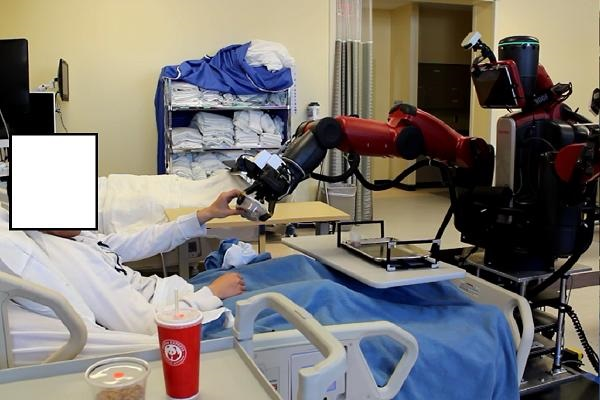
\includegraphics[width=0.48\linewidth]{fig//TRINARobot}
%   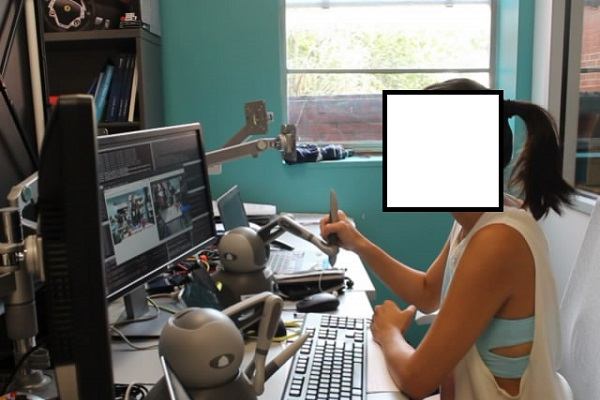
\includegraphics[width=0.48\linewidth]{fig//Operator}
%   }
% \caption{A tele-nursing robot that mediates between experienced teleoperator and end users (patients and nurse on-site) can develop its motion intelligence through learning from simultaneous multi-lateral physical human robot interaction, in order to provide adaptive assistance to novice teleoperator.}
% \label{MediatingRobot}
% \end{wrapfigure}
\paragraph*{Research Motivations:} 
Teleoperated medical robots enable collaborations between remote and on-site medical personnel as well as robot-mediated interactions with patients [ref]. These teleoperated robots often provide for greater safety, dexterity and effectiveness than existing autonomous robots, particularly on risk-sensitive tasks that require fine motor skills and contextual decision-making [ref]. 
However, providing expert teleoperation is a difficult task requiring attentiveness and large amounts of training.
In this project, we seek to reduce these challenges by providing user-adaptive assistance to novice teleoperators.
We plan to accomplish this by acquiring contextual motion intelligence from the robot-mediated collaborations/interactions between an expert teleoperator remotely controlling a teleoperated nursing robot and on-site nurses/patients.
%For a tele-nursing robot that mediates between human teleoperators and end users, it is efficient to acquire contextual motion intelligence through learning from the robot-mediated collaborations/interactions between an expert teleoperator and on-site nurses/patients, to provide user-adaptive assistance to novice teleoperators. 
Based on this idea, we propose a novel framework for \textbf{lifelong learning and fast adaptation for multi-lateral physical human robot interactions} (pHRI) that (1) integrates off-line and on-line learning of low-level motion skills and high-level task knowledge from demonstrations, and (2) uses this task knowledge to reason about (a) the human partner's desired subtask allocation as well as (b) the intentions of teleoperators and end users (c) to support appropriate task assistance or sub-task autonomy. Our research aims to improve the dexterity, customizability and usability of mobile humanoid nursing robots in performing complex collaborative tasks, and reduce the learning curve for novice users. The developed methods will more broadly benefit teleoperated robotic systems that operate in human environments for medical, industrial and social applications. 

% Such motion intelligence can be acquired as high-level models for task representation and decomposition as well low-level level 



% , with remote human partners in multi-lateral human-robot navigation and manipulation tasks---
% Teleoperation of this kind offers the potential to train models of desired  navigation and manipulation in these tasks that can %can be leveraged to 
% provide: %in a variety of ways to improve human-robot interactions. 
% (1) %develop the contextual motion intelligence of a mediating robot and (2) provide 
% user-adaptive assistance to novice teleoperators, reducing their effort for dexterous motion coordination; and
% (2) %enable 
% teleoperator-supervised robotic autonomy of some subtasks. 
% %Engaged in multi-lateral human-robot interactions, such robots are in an advantageous position to learn from the robot-mediated collaboration between its teleoperator and end user. 
% Our research %effort is %initially
% %motivated by the need 
% aims specifically to improve the dexterity and usability of mobile humanoid nursing robots in collaboration with human nurses and patients (see~\fig{Tasks}). 
% The developed methods will more broadly benefit tele-action robotic systems involving physical interaction with human partners that demand human-in-the-loop control due to task complexity, uncertainty and safety concerns.
%and perform tasks involving both navigation and manipulation in human environments and in intimate physical interaction with human partners.  

% \begin{figure}[h!!]
% \centering
% \vspace{-1em}
%   \mbox{
%   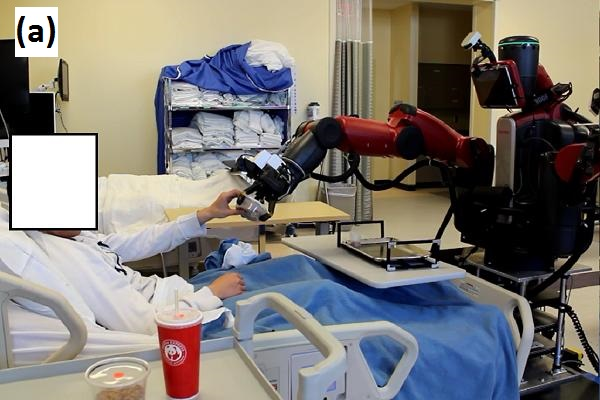
\includegraphics[width=0.16\linewidth]{fig//Task06}
%   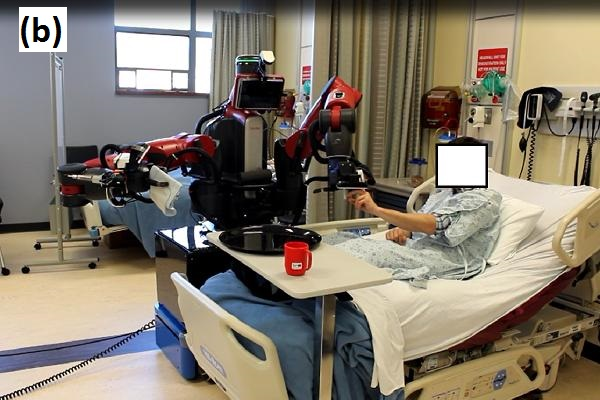
\includegraphics[width=0.16\linewidth]{fig//Task16}
%   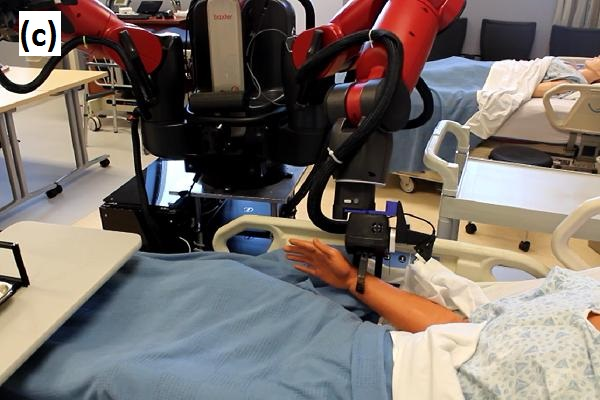
\includegraphics[width=0.16\linewidth]{fig//Task24}
%   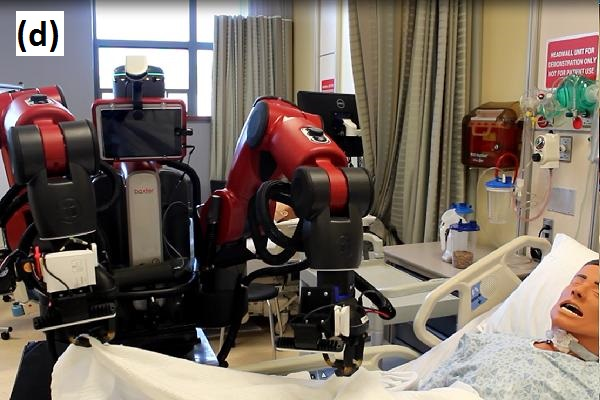
\includegraphics[width=0.16\linewidth]{fig//Task25}
%   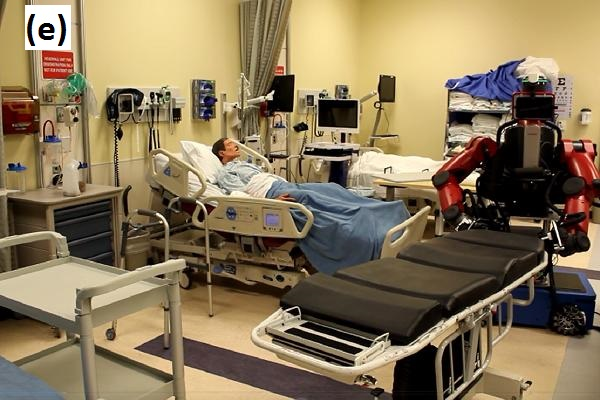
\includegraphics[width=0.16\linewidth]{fig//Task08}
%   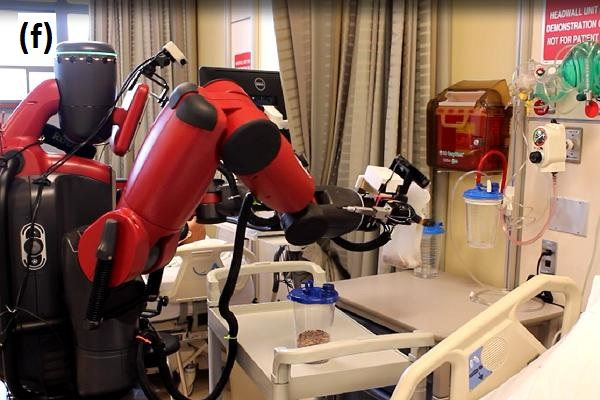
\includegraphics[width=0.16\linewidth]{fig//Task26}
%   }
% \caption{ A teleoperated nursing robot can develop its motion intelligence through learning from robot-mediated collaborations/interactions between (a) experienced teleoperator and end users (patients and nurses on-site). Our project focuses on collaborative and interactive and nursing tasks, such as (b) moving a patient transfer bed, (c.1-c.2) organizing and cleaning patient room, and (d.1-d.4) preparing and serving food to a patient.}
% \label{Tasks}
% \end{figure}

\begin{figure}[h!!]
\centering
% \vspace{-1em}
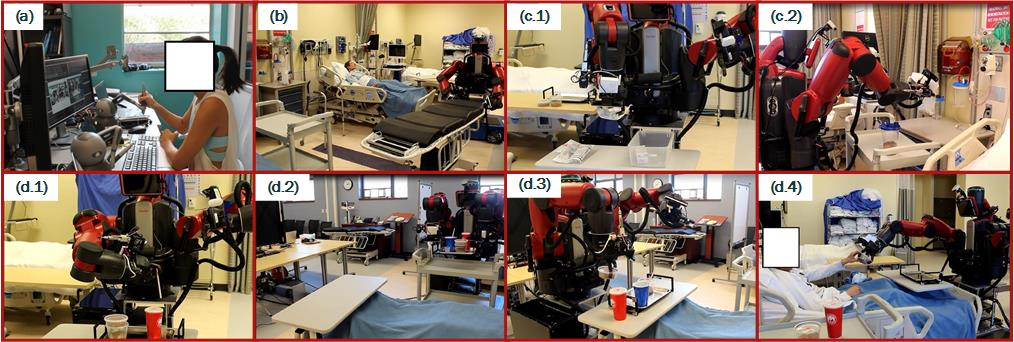
\includegraphics[width=0.99\linewidth]{fig//DemoTasks}
\caption{ A teleoperated nursing robot can develop its motion intelligence by learning from direct robot-mediated collaborations/interactions between (a) an experienced teleoperator and on-site patients and nurses. The nursing tasks we focus on include: (b) moving a patient-transfer bed, (c.1-c.2) organizing and cleaning the patient's room, which on-site nurses can perform more efficiently by collaborating with the teleoperated nursing robot, as well as (d.1-d.4) preparing and serving food to a patient, which involves inter-dependent task steps and intimate human-robot interactions. }
\label{Tasks}
\end{figure}

\paragraph*{Motivating Nursing Tasks:} This project focuses on frequently performed nursing tasks that could benefit from \textit{robot-mediated collaborations} between a teleoperator and an on-site nurse, such as moving a patient-transfer bed in a cluttered patient room (\fig{Tasks}(b)), organizing medical supplies (\fig{Tasks}(c.1)) and cleaning patient room debris (\fig{Tasks}(c.1)), as well as  \textit{robot-mediated interactions} between a teleoperator and a patient, such as food preparation and serving. Under direct teleoperation, these tasks are feasible for a mobile humanoid nursing robot to complete, although task completion time is about 95x times slower than direct human performance~\cite{Hauser_Li_TRINA:17}. Despite the existence of bilateral telepresence, it is still difficult for teleoperators to communicate complex motion intents, which are essential for intimate collaboration. When telepresence communication is frequent, attention to maintaining video/audio communication channels may distract and slow down the teleoperators' control of the robot, adding to the their perceptual burden~\cite{Hauser_Li_BiTelepresence:17}. So far, no data is available for the feasibility and performance of these tasks under fully autonomous or supervisory control. However, existing research in the field of robot motion planning, robot learning and human-robot interactions, have revealed that the challenges in this tasks are many and significant. 

\paragraph*{Challenges}: This research aims to address three main challenges. \underline{\textbf{\textit{For the mediating robot}}}, {\it neither direct teleoperation nor fully-autonomous control are ideal options}; direct teleoperation often lacks precision for fine-grained control enabled by combining on-site sensing information ~\cite{chen2007human,chen2011supervisory}, while pure autonomy often cannot appropriately interpret highly collaborative and interactive tasks with human partners~\cite{beer2014toward,nahavandi2017trusted,alaieri2016ethical}. \underline{\textbf{\textit{For end users}}}, such as patients and on-site human nurses, {\it physical interactions and collaborations are difficult because robot autonomy may not appear natural and fluent}~\cite{goetz2003matching,strabala2013towards, mitsunaga2008adapting}. This unexpected robot behavior may confuse, surprise or even intimidate end users, adding to patient stress, discomfort and/or anxiety~\cite{nomura2008prediction}. \underline{\textbf{\textit{For the teleoperator}}}, controlling a mobile humanoid robot to perform dexterous coordinated motions involves a {\it significant learning curve for novice users to adapt to the low transparency of the teleoperation system and physical capabilities of the robot}~\cite{rosen2002task,ballantyne2002robotic,novick2003analysis,sudan2012multifactorial,sng2013multiphasic}. This prevents nurses, who have significant first-hand experience and task knowledge, from effectively teleoperating a different physical embodiment.
In addition, perceiving the remote environment to control position and orientation precisely is difficult despite having many available static and dynamic camera views. The novice teleoperators' high-level task knowledge of task goals, procedures, and object affordances are still valid, but the low-level motion primitives and their coordination,  as well as the motion-perception mapping have to be relearned through the significant practice. 


% coordinated and dexterous manipulations [ref], navigation in cluttered human environments [ref], fluent and natural-looking human-robot collaborations [ref] and interactions [ref], intent inference in human-robot interactions [ref] have revealed that the challenges in this tasks are not trivial. 


% \textit{robot-patient interactions}, such as preparing and serving food, taking vital sign measurements from patients and adjusting patients' bodies, as well as (2) \textit{robot-nurse collaboration} in which the robot assists a human nurse to clean a patient's room, collect and organize medical supplies, and move portable medical devices (e.g., patient transfer bed). Shown in~\fig{Tasks}, Tasks (a)-(c) involve delicate and intimate interactions with a patient, while the nursing robot collaborates closely with an on-site nurse in Tasks (d)-(f). We expect these demonstration tasks can best evaluate the contextual motor skills learned, and demonstrate the system's capability of inferring shared user intentions when assist novice teleoperators.

% \paragraph*{Challenges}: This research aims to address three main challenges %unique  %% BDZ: probably general to other human-in-the-loop settings
% for robot-mediated collaborative nursing tasks. 
% \underline{\textbf{\textit{For the mediating robot}}}, {\it neither direct teleoperation nor fully-autonomous control are good options}; direct teleoperation often lacks precision for fine-grained control enabled by combining on-site sensing information ~\cite{chen2007human,chen2011supervisory}, while pure autonomy often cannot appropriately interpret highly collaborative and interactive tasks with human partners~\cite{beer2014toward,nahavandi2017trusted,alaieri2016ethical}.
% %We propose to overcome these limitations by leveraging the benefits of {\bf human teleoperation primarily at higher-levels of task abstraction} and the benefits of {\bf autonomous control primarily at lower-levels of task abstraction}.
% %, the mediating robot could not utilize on-site sensing information to perform precise low-level control, but have to execute the trajectories commanded by the teleopertor the based on their inaccurate or even distorted perception through camera views. On the other hand, it is also beyond the robot's capability to autonomously handle highly collaborative and interactive tasks.  
% %To participate as a competent partner, an autonomous robot needs to understand its dynamic and contextual task-sharing and decide when and how to help. It also needs understand the role it can play based the intention and preference of the human partner.   
% \underline{\textbf{\textit{For end users}}}, such as patients and on-site human nurses, {\it physical interactions and collaborations are difficult because robot autonomy may not appear natural and fluent}~\cite{goetz2003matching,strabala2013towards, mitsunaga2008adapting}. This unexpected robot behavior may confuse, surprise or even intimidate end users, adding to patient stress, discomfort and/or anxiety~\cite{nomura2008prediction}.
% %We propose to avoid ``unnatural'' autonomous robotic behavior by {\bf learning motion primitives from expert teleoperation demonstrations}, which are more natural, and to then adapt these in a user-acceptable manner to new situations.
% \underline{\textbf{\textit{For the teleoperator}}}, controlling a mobile humanoid robot to perform dexterous coordinated motions %is a non-trivial task. It demands a 
% involves a {\it significant learning curve for novice users to adapt to the low transparency of the teleoperation system and physical capabilities of the robot}~\cite{rosen2002task,ballantyne2002robotic,novick2003analysis,sudan2012multifactorial,sng2013multiphasic}. This prevents nurses, who have significant first-hand experience and task knowledge, %cannot easily apply their experience of performing nursing tasks with their own hands, and instead have to explore new motion coordinations when controlling a different physical embodiment.
% from teleoperation that effectively controls the different physical embodiment.
% In addition, perceiving the remote environment to control position and orientation precisely is difficult despite having many available static and dynamic camera views. The teleoperators' high-level task knowledge of task goals, procedures, and object affordances are still valid, but the low-level motion primitives and their coordination,  as well as the motion-perception mapping have to be relearned through the practice of teleoperation. 

\begin{wrapfigure}{r}{3.0in}
\centering
  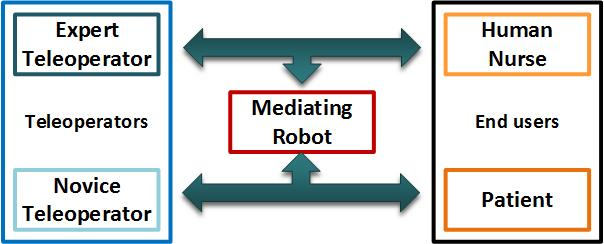
\includegraphics[width=0.99\linewidth]{fig//001TeleNursing_Overview}
\caption{Learning from robot-mediated multi-lateral physical human-robot interactions.}
\label{001TeleNursing_Overview}
\end{wrapfigure}

\paragraph*{A Novel Framework for Robotic Mediation Between Teleoperators and End Users:} We propose to address the above challenges by leveraging the benefits of {\it human teleoperation primarily at higher-levels of task abstraction} and the benefits of {\it autonomous control primarily at lower-levels of task abstraction}. Shown in~\fig{001TeleNursing_Overview},  our approach is enabled by the key idea of {\bf observing how a mobile humanoid robot equipped with a human mind (of an expert teleoperator) behaves when interacting with and collaborating with people.} In this learning context, the teleoperator and end user adapt to each other and setup a feasible and potentially optimal collaboration paradigm given the physical capability of the teleoperated robotic system. Their joint effort demonstrates to the mediating robot the big picture of task collaboration, and the role it can play as a competent participant. 

% We develop lifelong learning techniques for forming and refining high-level task knowledge and low-level motion primitives from demonstrated expert teleoperation for the nursing tasks of~\fig{Tasks}. 

\paragraph*{Objectives:} Our research activities pursue three objectives: 

% This project aims to (1) develop the motion intelligence of a mediating robot through learning from multi-lateral physical human-robot interaction, and (2) utilize such motion intelligence to assist novice teleoperator. 

\begin{itemize}
\item \textbf{Objective 1} --- Enable robot to acquire contextual and customizable task knowledge and motion skills through lifelong learning from collaborative multi-lateral physical human-robot interaction tasks. 
\end{itemize}
\noindent
Our proposed \textbf{lifelong robot learning approach} aims to overcome the limitations of autonomous motion planning [cite] and robot learning methods [cite], and integrate their advantages into the framework of multi-lateral physical human-robot interactions/collaborations. In this framework, a mediating robot observes the contextual interaction/collaboration between an expert teleoperator and end users, and continuously acquires and updates its high-level task knowledge and low-level motion skills. At high-levels, the robot can learn abstract representation of task structure~\cite{} and probabilistic models that relate actions and effects~\cite{}. It can also learn the object affordance for individual and joint actions~\cite{knoblich2011psychological}. At low-levels, the mediating robot can acquire contextual motion skills such as the motion primitives and their temporal-spatial coordination. Such motion skills can be directly used for robot motion reproduction, since it considers the effects of robot physical embodiment and the transparency of teleoperation interface, which cannot be learned from observing human-human interactions. It also naturally addresses the inter-adaptive phase matching between human and robot and therefore differs from robot learning without human partners. More importantly, our proposed approach integrates learning both on- and off-line so that robot behavior can be customized with minimal online demonstrations or human teaching efforts. To account for both behavior robustness and fast adaption, our method compares new demonstrations with the existing models of task representation and motion skills. Efficient incremental learning will be performed if no significant differences are observed. Otherwise, the robot will perform significant update task and motion skill models, after confirming with the human user. 

\begin{itemize}
\item \textbf{Objective 2} --- Develop fast intention forecasting approaches for user-adaptive task-sharing, joint performance optimization, real-time motion prediction and recognization. 
\end{itemize}

\noindent
The \textbf{systematic approach for fast intent inference} we propose enables learning the rewards and constraints that govern (1) the motion coordination under shared autonomous control, and (2) the dynamic task-sharing of robot-mediated nursing tasks that result from the explicit negotiation and implicit adaption between a teleoperator and end user. For instance, the robot can also learn \textit{motion coordination strategies} such as how to autonomously move the mobile base to facilitate the manipulation when moving a patient transfer bed with a human nurse. It can also learn \textit{collaboration strategies}, such as where to grasp on the patient transfer bed given where the human nurse grasps, and how to push the patient transfer bed to assist the human nurse's motion. Besides inferring task rewards and constraints, we are also interested in real-time motion prediction using inference about an end user's intent, so that the robot can behave pro-actively and naturally in interactions with patients. As an adaptation for novice teleoperators, we propose an \textit{active intent detection method} to infer the operation a novice intends to perform, and autonomously control the low-level motions accordingly.

% learned collaborative task decompositions and cooperative inverse reinforcement learning.

% Key idea: Lifelong learning; fuse imitation and reinforcement learning; game theory

\begin{wrapfigure}{r}{3.5in}
  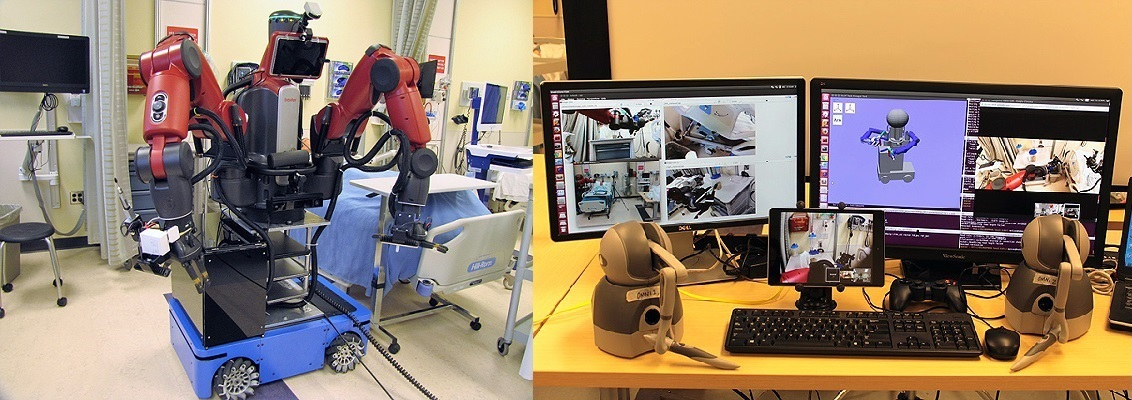
\includegraphics[width=0.99\linewidth]{fig//TRINA_system}
    \caption{(Left) The Tele-robotic Intelligent Nursing Assistant (TRINA) system and (Right) its operator console which can support direction teleoperation and shared-autonomous control.}
    \label{fig:Trina}
\end{wrapfigure}
\begin{itemize}
\item \textbf{Objective 3} --- Implement lifelong robot learning and fast intent inference on the Tele-robotic Intelligent Nursing Assistant (TRINA) system, and demonstrate their performance on assisting novice teleoperators in robot-mediated interactions/collaborations. 
% and blended control algorithms for user-adaptive assistance that optimize the multiple objectives of: sub-task performance, gathering information of user intent, and interpretability of robotic control to the end user. 
\end{itemize}

\noindent
We plan to implement our proposed methods for lifelong learning and fast intent forecasting on a mobile humanoid nursing robot platform (\fig{fig:Trina}) and validate their efficiency through in-lab testing over demonstration of three collaborative and interactive nursing tasks (\fig{Tasks}). With the support of NSF grants (NSF RAPID \#IIS-1513221 and NSF CAREER \#1253553), our previous work developed this Tele-robotic Intelligent Nursing Assistant (TRINA) system to minimize the risks of exposure to highly infectious diseases among healthcare workers like nurses, Emergency Medical Technicians (EMTs) and aid workers during outbreaks (e.g., Ebola and Zika epidemics of 2014--2016). This nursing robot platform consists of two compliant 7 DoF on a humanoid torso (Rethink Robotics Baxter), an omnidirectional mobile base (HStar AMP-I), and three-fingered grippers (Righthand Robotics ReFlex grippers) on each hand to enable manipulation and indoor navigation capabilities. It is also equipped with a variety of sensors for visual feedback and environment mapping, and devices for bidirectional telepresence. Under direct teleoperation, this nursing robot can act as a surrogate for medical personnel to perform frequent light- to medium-duty caregiving tasks in quarantine environments~\cite{Hauser_Li_TRINA:17}. More importantly, the development of tele-nursing approaches promises a future that synergizes the capabilities of robots and remote medical personnels to improve the quality, availability, and affordability of healthcare. Through user studies we will evaluate whether the system can (1) efficiently acquire task knowledge and motion skills from experts, (2) provide user-adaptive assistance in robot-mediated interaction/collaboration, and (3) reduce the learning and operation barriers for novice teleoperators. 

% \paragraph*{Platform} Shown in~\fig{fig:Trina}, this nursing robot consists of a dual-armed humanoid torso (Rethink Robotics Baxter), an omnidirectional mobile base (HStar AMP-I), and three-fingered grippers (Righthand Robotics ReFlex grippers) on each hand to enable manipulation and indoor navigation capabilities.  A telepresence screen, microphone, and speakers provide bidirectional audio/visual communication between operator, patients, and other healthcare workers at the remote site. The power cable roller has a 30-foot extension cord that retracts and locks at any length, providing a large enough range of motion to traverse a typical hospital room. A variety of sensors situated on the robot provide visual feedback, including the built-in ultrasonic rangefinders to detect people in the robot's vicinity, a Microsoft Kinect 2 attached to the robot's chest, two Intel RealSense F200 3D cameras attached to the robot's wrists, two Huokuyo LIDAR sensors attached to the mobile base. All of the RGB+D/LIDAR sensors contribute to building 3D maps of the environment, which are provided to the operator's console. Four computers are mounted on the robot's chassis, one for motion control and three for vision processing.


\paragraph*{Intellectual Merits:} Our proposed research aims to address the need for \textit{\textbf{developing contextual, user-adaptive and evolvable robot motion intelligence}}. Our preliminary work has evaluated the capability of TRINA over frequently performed nursing tasks in a simulated patient room~\cite{Hauser_Li_TRINA:17}. Under direct teleoperation, TRINA is capable of performing many nursing tasks that are still not feasible for autonomous control, yet the robot task completion times are far more longer than those of human nurses. This is mostly due to the teleopeartors' difficulties in (1) learning the perception mapping to infer the spatial relationship from multiple camera views, and (2) learning motion mapping from an input device to the robot to perform precise motion control and motion coordination. Despite of the perception and motion control challenges, human teleoperators are still superior in high-level task planning, task performance evaluation (if the task is performed to the level of satisfaction), correction (updating plans based on current task status) and interactive response. A paradigm of shared-autonomous control or supervisory control will combine the human capability of decision making, task performance evaluation, and correction, with the robot's capability of perception and motion control accuracy. Thus, it is necessary to equip the teleoperated nursing robot with the capabilities of lifelong learning and fast intent forecasting, to develop contextual motion intelligence through robot-mediated interactions between expert teleopertors and end users, and evolve its motion intelligence accordingly to new task demonstrations and user preferences, and provide user-adaptive assistance to novice teleoperators. This motion intelligence will reduce learning and operation efforts for teleoperated nursing robot control, and improve the customizability of nursing robots, lowering barriers for medical personnel to use teleoperated nursing technologies. 

% \todo{Jane: I have finished revision until here!}

% , in the tasks that have complicated structures and/or involve collaborative/interaction manipulation of a shared object. 
% while staying near the collaborative end user and avoiding people passing by. 

% At low-level, the mediating robot can acquire from the teleoperator the knowledge of the motion primitives and their temporal-spatial coordination. Such knowledge can be directly applied to low-level motion reproduction in pHRI, for its considers effect of robot physical embodiment and the transparency of teleoperation interface, which can not be learned from interactions between humans. It also naturally addresses the inter-adaptive phase matching between human and robot and therefore differs from robot learning without human partners. 

% Our key idea is to let the robot observe how a robot embodiment equipped with a human mind behaves when interacting and collaborating with humans. 


% \begin{wrapfigure}{r}{3.0in}
% \centering
%   \includegraphics[width=0.99\linewidth]{fig//001Task_Overview_}
% \caption{Task overview.}
% \label{001Task_Overview}
% \end{wrapfigure}


% This task involves implementing the proposed motion control strategies on a humanoid nursing robot, and conducting a user study to evaluate their efficacy. The user study will recruit 20 subjects to operate the robot with and without the assistance of the autonomous coordination of the manipulator arm with its micro-structures and evaluate whether such coordination can improve task performance and user experience.

% \paragraph*{Objectives:} This project aims to (1) develop the motion intelligence of a mediating robot through learning from multi-lateral physical human-robot interaction, and (2) utilize such motion intelligence to assist novice teleoperator to coordinate the mobile base with the manipulator arms and to perform dexterous coordinated manipulation. To achieve these goals, this project will pursue the following research objectives: 

% \begin{itemize}
% \item \textbf{Objective 1} --- Enable lifelong learning for collaborative  multi-lateral physical human-robot interaction tasks through learned collaborative task decompositions and cooperative inverse reinforcement learning.

% % Key idea: Lifelong learning; fuse imitation and reinforcement learning; game theory

% \item \textbf{Objective 2} --- Develop fast intention inference and blended control algorithms for user-adaptive assistance that optimize the multiple objectives of: sub-task performance, gathering information of user intent, and interpretability of robotic control to the end user. 

% \item \textbf{Objective 3} --- Develop, implement, and evaluate intelligent shared-autonomous control modules to assist novice teleoperators in navigation and dexterous manipulation.  

% % \begin{itemize}
% % \item Develop autonomous navigation strategy to facilitate manipulation tasks

% % \textbf{Key idea}: Lifelong learning; fuse imitation and reinforcement learning; game theory 
% % item Develop adaptive manipulation assistance based on inferring of motion intent of novice teleoperator

% % \textbf{Key idea}: Coordination of macro- and micro-structure; Coordination policy hypothesis: manipulability, reachability, vision advantage (perception convenience and comfort); minimal intervention of macro-structure (also relevent to energy consumption); environment constraints (static obstacle, prediction of moving obstacle and agents)

% % \end{itemize}

% \end{itemize}

\noindent

% \paragraph*{Intellectual Merits}

% \paragraph*{Broader Impacts}


\paragraph*{PI's Qualifications}
PI Zhi Li has worked on motion planning and learning for human-compatible and human-like medical robots, including exoskeletons for rehabilitation, arm-like surgical robots and nursing robots, and has spread to the mechanical design optimization~\cite{li2016design}, teleoperation and haptics~\cite{li2009networked,li2009remote}, and physical human-robot interaction~\cite{li2017study}. Related to this proposed project, she has studied reward function that governs the regularity and variability of reaching and reach-to-grasp motions in a 3D workspace, and developed mathematical models that can accurately predict human arm postures in real-time~\cite{kim2012resolving,Rosen_Li_EMBC:13,Rosen_Li_IROSChapt:13,Rosen_Li_IROS:14,Rosen_Li_J:14, li2017reaching}. Li's motion learning and prediction algorithm can resolve the kinematic redundancy of a dual-arm rehabilitation exoskeleton, enable it to render arm postures that are fully compatible with healthy operators, and correct abnormal joint coordination due to motor disability. She also developed the Tele-robotic Intelligent Nursing Assistant (TRINA) system, and conducted system capability evaluation under direct teleoperation~\cite{Hauser_Li_TRINA:17}.

PI Jie Fu's research focuses on planning and control synthesis of verifiable robotic systems. Her thesis work developed a symbolic method for abstraction-based control of hybrid systems that enables scalable planning for complex behaviors under temporally and spatially dependent tasks \cite{fu2013bottom}. Fu introduces grammatical inference \cite{fu2014adaptive} as a behavior inference method to enable adaptive symbolic planning in task space. In recent work, Fu developed a  planning method for a class of stochastic shared autonomous systems, featuring  human-robot task sharing \cite{fu2016synthesis}. This research effort allows the system to achieve Pareto-optimality for system  performance while balancing against human efforts. Other related  work  includes game theoretic planning for multi-agent systems under  temporal logic tasks \cite{fu2015concurrent} and approximate optimal control under temporal logic constraints, which include common temporally extended goals \cite{fu2017sampling}.

PI Brian Ziebart is an expert in structured prediction methods for sequential behavior.  Ziebart developed maximum entropy inverse reinforcement learning (MaxEnt IRL) \cite{ziebart2008maximum,ziebart2010modeling} to learn the utilities motivating demonstrated behaviors while simultaneously providing robust prediction guarantees. 
Ziebart's projects based on these methods have enabled more accurate predictions of user intent in pointing tasks for graphical user interfaces \cite{ziebart2012probabilistic}, physical motions \cite{monfort2015intent}, and teleoperation \cite{schultz2017goal}.
Recently, Ziebart has developed methods for accelerating predictions of these methods using ideas from heuristic-guided search \cite{monfort2015softstar} and hybrid decompositions of the state space \cite{byravan2015graph}.


%-------------------------------------------------------------------------
\section{Related Work}\label{sec:related}
%-------------------------------------------------------------------------

% %-------------------------------------------------------------------------
% \subsection{Background --- Toward a robotic nursing assistant of motion intelligence}\label{sec:related-TRINA}
% %-------------------------------------------------------------------------


% \noindent
% The rapid development of telerobotic approaches promises a future that synergizes the capabilities of robots and remote medical personnel to improve the quality, availability, and affordability of healthcare. For example, these technologies minimize the risks of exposure to highly infectious diseases for  healthcare workers like nurses, Emergency Medical Technicians (EMTs), and aid workers during outbreaks, such as the Ebola and Zika epidemics of 2014--2016. With the support of NSF grants (NSF RAPID \#IIS-1513221 and NSF CAREER \#1253553), our previous work developed the Tele-robotic Intelligent Nursing Assistant (TRINA) system to act under teleoperation as a surrogate for medical personnel to perform frequent light- to medium-duty caregiving tasks in quarantine environments~\cite{Hauser_Li_TRINA:17}.

% \paragraph*{Platform} Shown in~\fig{fig:Trina}, this nursing robot consists of a dual-armed humanoid torso (Rethink Robotics Baxter), an omnidirectional mobile base (HStar AMP-I), and three-fingered grippers (Righthand Robotics ReFlex grippers) on each hand to enable manipulation and indoor navigation capabilities.  A telepresence screen, microphone, and speakers provide bidirectional audio/visual communication between operator, patients, and other healthcare workers at the remote site. The power cable roller has a 30-foot extension cord that retracts and locks at any length, providing a large enough range of motion to traverse a typical hospital room. A variety of sensors situated on the robot provide visual feedback, including the built-in ultrasonic rangefinders to detect people in the robot's vicinity, a Microsoft Kinect 2 attached to the robot's chest, two Intel RealSense F200 3D cameras attached to the robot's wrists, two Huokuyo LIDAR sensors attached to the mobile base. All of the RGB+D/LIDAR sensors contribute to building 3D maps of the environment, which are provided to the operator's console. Four computers are mounted on the robot's chassis, one for motion control and three for vision processing. 

% \jie{include a description on how you want to improve the mechanical design of the precise positioning unit.}




% and develop user-adaptive assistive modules to . For instance, a tele-nursing robot of such motion intelligence would rather interpret and process their operation of input devices as high-level motion intent (e.g., reaching towards an object), instead of execute as direct command (e.g., the robot end-effector trajectory). 


% Direct teleoperation of a nursing robot demands so much perception and motion control efforts that a teleoperating nurse may not be able to spare attention to the communication with a patient, which is essential in patient-caring~\cite{Hauser_Li_BiTelepresence:17}. 

% \paragraph*{A nursing of motion intelligence} Despite of the above perception and motion control challenges, 




% Due to significant challenges perception and motion control, even an expert teleoperator teleoperated robot cannot behave fluently and naturally in terms of arm posture and the timing of its responses When interacting with a human end users. 






% Here we present the perception and motion control challenges observed in the direct teleoperation of nursing tasks~\cite{li2017development}: 






% \noindent
% (1) Perception Challenge --- Human teleoperator perceives the task and environment primarily through robot cameras, and has deep learning curve for estimating the spatial relationship from fixed and/or moving camera view: fixed camera has limited vision range and perspective, while moving camera poses challenges in estimating object spatial relationship, particularly for distance and orientation. On the other hand, the nursing robot on-site can observe the task directly and in close distance; It is also capable of accurately perceiving the spatial relation (e.g. object position, relative distance), and motions (e.g. the estimated speed of a moving object).

% \noindent(2) Motion challenges --- Novice teleoperators have many difficulties in controlling the coordination of many degrees of freedom. It is hard to control dexterous motions that require coordination between two arms, between arm and hand, or between manipulator arms and mobile base navigation. In addition, It takes significant efforts to learn the mapping from input device operation and robot motions, particularly for precise control of  orientation. To novice teleoperator, controlling relative motion (moving left/right, further/close with respect to reference object) is easier than controlling absolute motion (moving to a specific x, y, z). They cannot distinguish/control motions that slightly differ in velocity and direction very well. Due to significant challenges in motion control, a teleoperated robot cannot behave fluently and naturally in terms of arm posture and the timing of its responses When interacting with a human end users. Direct teleoperation demands overwhelming control effort such that a teleoperating nurse do not have very much attention to communicate with a patient, which is an essential component of patient-caring. 



% Therefore, the teleoperation system  The proposed user assistive module aims to combine the human capability of decision making and task performance evaluation, correction, with the robot's capability of perception and motion accuracy. To justify the design of user assistive module, here we present the perception and motion control challenges observed in the direct teleoperation of nursing tasks~\cite{li2017development}:

% it is difficult for  it is still challenging for novice users to learn the spatial relationships of the workspace from a combination of static and moving camera views. 

% Despite our efforts in developing an informative, versatile, and intuitive user interface, 



% To address the above challenges, 

% For instance, the teleoperation system would rather interpret and process their operation of input devices as high-level motion intent (e.g., reaching towards an object), instead of execute as direct command (e.g., the robot end-effector trajectory). The proposed user assistive module aims to  To justify the design of user assistive module, here we present the perception and motion control challenges observed in the direct teleoperation of nursing tasks~\cite{li2017development}: 
% \jie{This problem formulation should be merged with task 2.}

% It  the strength of human and robots in perception and motion control while compensating the weakness of each other. 

% \jie{need a mathematical formulation. Related: intention-aware motion planning in mixed-observation MDP. However, the challenge is that novice users's demonstration can be errornous. Potentially we can propose to use expert demonstrations to infer the intention of novice users, based on human motion similarity. May relate to Co-active learning.}



% \paragraph*{Lessons learned:} The limitations revealed in previous capability evaluations show that it is necessary to endow the nursing robot with motion intelligence to understand collaborative task decompositions and assignments, and to provide adaptive assistance based on the human teleoperator/partner's level of skill. In multi-lateral pHRI, collaborative task decomposition not only concern what operation a shared object can afford, but also the dynamic task-sharing between the teleoperated mediating robot and the human partner on-site. From expert teleoperator and end user, a mediating robot can observe their robot-mediated collaboration to acquire high-level models for the collaborative task decomposition, including the \textit{dynamic task-sharing} and \textit{shared object affordance}. It can also learn low-level models for movement primitives and their temporal-spatial coordination, to automate the precise low-level control based on the explicit and/or implicit user intentions.  

% \jie{In this paragraph, we need to clarify which tasks are teleoperated. For example, dexterous in-hand manipulation may be autonomous while the user tele-operate macro-action. this is to remove the concern that we will track users' figure to perform tele-op of robot hand.}




%-------------------------------------------------------------------------
\subsection{Lifelong learning through human-robot interactions}\label{sec:related-learning}
%-------------------------------------------------------------------------


% \begin{figure}[h]
% \begin{center}
% 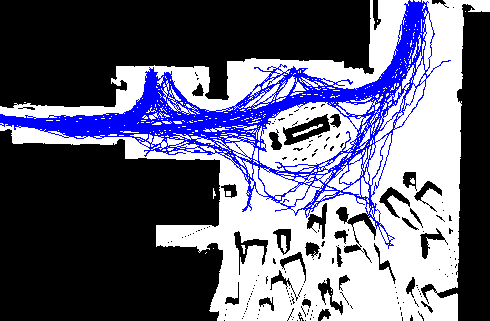
\includegraphics[width=2in]{fig/trajectories.png}
% 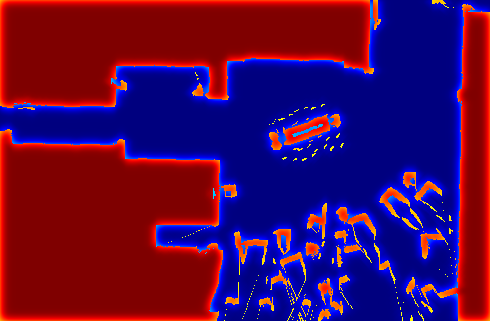
\includegraphics[width=2in]{fig/learned_cost.png}
% 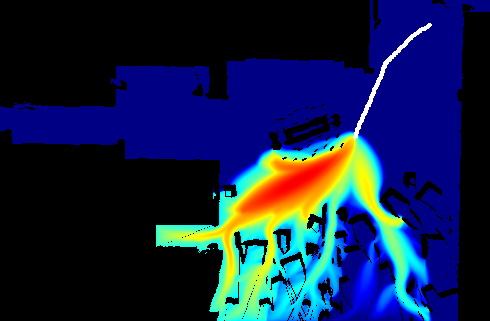
\includegraphics[width=2in]{fig/forecast.png}
% \end{center}
% \caption{(left) Users' trajectories within an environment. (center) A learned cost function explains trajectories as solutions to plans (red is high cost). (right) A forecast of future trajectories (red is most likely).}
% \label{fig:forecast}
% \end{figure}


Programming robots to appropriately perform nursing tasks across a wide range of contexts is a daunting undertaking.  
Automatically learning in a flexible manner is far more desirable.
Lifelong learning for robotics \cite{thrun1995lifelong,thrun1995lifelong2,thrun1998lifelong} seeks to incrementally and continuously learn knowledge from some tasks that can be transferred to other tasks. 
It has been more recently applied for the open-ended task of reading the web to collect relational facts \cite{banko2007strategies,carlson2010toward}. 
However, formulations based on classical machine learning paradigms, though appealing in theory, are ill-suited.
Reinforcement learning, for example, would require inordinate amounts of
feedback (including feedback for negative outcomes)
before appropriate behaviors could possibly be realized.
To avoid this difficulty, we propose lifelong learning based on directly learning appropriate assistive behavior from the demonstrations of the expert teleoperator.
Though many forms of imitation learning exist \cite{argall2009survey}, we focus on the following methods: (1) {\bf learning dynamic motion primitives} \cite{matsubara2011learning,kulic2012incremental} that can be adapted for new contexts, (2) \textbf{learning abstract task representations} for high-level task reasoning and generalization~\cite{niekum2013semantically,konidaris2012robot,konidaris2018skills}, (3) learning object affordance that constrains the individual and joint actions~\cite{aksoy2011learning,knoblich2011psychological,shu2017learning}, and (3) {\bf inverse reinforcement learning} \cite{ng2000algorithms,abbeel2004apprenticeship}, which seeks utility functions that make demonstrations rational in sequential decision and control processes.

%-------------------------------------------------------------------------
\subsection{Intent forecasting in robot-mediated interactions}\label{sec:related-learning}
%-------------------------------------------------------------------------

Intent inference endows robots with socially appropriate and natural-looking behaviors and improves the fluency of human-robot interactions~\cite{calinon2009learning,strabala2013towards}. Instead of inferring intents from more intentional and explicit cues (e.g., gaze, body gestures~\cite{huang2016anticipatory}), inferring the implicit intent encoded in human motion may be more efficient and less intrusive, since it minimizes end user effort for maintaining explicit or even exaggerated human-robot communication. At a low-level, a robot can predict its human partner's motion based on the knowledge of tempo-spatial coordination observed in individual and interaction human motions~\cite{Hogan_Flash:85, sisbot2012human,huber2010assist, glasauer2010interacting, strabala2013towards, li2015rssworkshop, perez2015fast,maeda2017phase}. At a high-level, the intent inference problem can be formulated as inferring the parameters of a dynamic model~\cite{wang2013probabilistic}, Bayesian network~\cite{liu2016fuzzy} or Markov decision process~\cite{mcghan2015human} and tackled using techniques such as inverse linear-quadratic regulation (ILQR)~\cite{monfort2015intent} and approximate expectation-maximization~\cite{ravichandar2017human}. However, given the state-of-the-arts methods for motion prediction and motion intent inference haven't fully considered that towards a successful collaboration, \textit{the collaborative partners do not necessarily insist their initial intents and plans, but will adjust based on the explicit negotiation of task-sharing and/or inter-adapation of each other's capability}~\cite{nikolaidis2017human}. In human-robot interactions, it is quite usual that humans adapt too much to the robot for they do not trust robot's task experience and decision-making intelligence. They are also not clear about the robot can achieve given its physical capability and therefore make conservative assumption for task sharing. Although the collaborative task succeeds, robot may end up with little contribution towards their shared goal, and even perform lower than their potential~\cite{hancock2011meta,lee2013computationally,salem2015would}. \textit{Our proposed framework of learning from robot-mediated interactions is very effective method to fix this problem}: An expert teleoperator will not only endow the mediating robot with the human-level intelligence for decision-making, but can also investigate how to fully exploit its physical capabilities in interactive/collaborative tasks. From a human partner's perspective, it is also convenient to negotiate with the teleoperator for the optimal task-sharing, and establish an ideal collaboration paradigm for the mediating robot to perform the task under shared autonomy.  

% It can also be modeled as a Markov decision process so that the human partners' future course of action based on the knowledge of the human partner's goal sequences, recent action history, and observed correlation between behaviors with actions~\cite{mcghan2015human}.



%-------------------------------------------------------------------------



% The natural separation of macro- and micro-structures in human arms has inspired the development of robotic manipulators with macro- and micro-structures~\cite{Nagai:94,Murakami_Yoshikawa:93}. 
% However, little work has been done to relate the control strategy for coordinating macro- and micro-structures with the motion studies on human arm-hand-finger coordination. For example, human motion studies have revealed that a reach-to-grasp motion can be constructed from a reaching motion toward the same target position. If the target orientation is perturbed when the hand is still approaching to the target, the hand path will remain approximately the same, while the hand orientation will be gradually turned from the one that matches the original target orientation to the one that matches the new target orientation~\cite{Tillery_Fan:06}. The PI's research on reach-to-grasp motions further pointed out that (1) the arm posture will adjust to accommodate the grasping hand pose, and (2) if there exist multiple DOFs that can be used to satisfy the same task specification (e.g., the grasping orientation in one dimension), the DOFs of the macro-structure will be largely unused until the DOFs of the micro-structure have been mostly exploited. On the other hand, redundancy resolution strategies have been proposed for flexible-macro/rigid-micro manipulators~\cite{Yoshikawa_Nakamura:87,lew1995micro}, compliant base manipulators~\cite{lew2001simple}, and coarse/fine dual-stage manipulators~\cite{kumar2000augmentation, kwon2001coarse,dong2008stiffness}, so that the macro- and micro-structures can compensate each other in terms of precision and motion range. The redundant DOFs can be used to resist perturbations/vibrations~\cite{lew1995micro, kwon2001coarse}, and they can also enable the micro-structure to satisfy additional task constraints or to maintain a desired level of manipulability~\cite{Yabuta_Quan:06,Yabuta_Huang:06,Yabuta_Huang:10}. These motion coordination strategies cannot render natural-looking motions and therefore cannot be directly applied to coordinating the arm and hand of humanoid and human compatible robots when human-like motion is desired. The existing research efforts are also limited by their focus on individual reaching or grasping tasks. It is unclear when and how to move which parts of the robot to better perform tasks in sequence, tasks in a group, and tasks that require different motor skills, or to be better prepared for unexpected tasks.

%-------------------------------------------------------------------------
\section{Research Plan}\label{sec:plan}
%-------------------------------------------------------------------------

Our research plan is divided into three activities: developing lifelong learning approaches to acquire and evolve task knowledge and motion skills (Activity 1); developing fast fast intent forecasting methods to assist the robot-mediated collaborations/interactions between novice teleoperator and end users (Activity 2); and implementing the proposed methods and evaluating their efficiency in collaborative/interactive nursing tasks (Activity 3).

%-------------------------------------------------------------------------
\subsection{Activity 1 --- Lifelong learning of multi-lateral physical human-robot interaction}\label{sec:plan-motion}
%-------------------------------------------------------------------------
\noindent


%Goals: %\textbf{Learning from robot-mediated multi-lateral physical human-robot interactions/collaborations, to acquire knowledge of collaborative task decomposition.} 
\noindent
{\bf Problem statement:} In our first research activity,
{\bf we seek to construct task knowledge and motion skills from the robot-mediated collaboration demonstrated by expert teleoperators and end users}. We propose to: use motion primitives to model and generalize the temporal and spatial coordination in individual robot motions and between end users and teleoperated robots (Activity 1.1); use automaton learning method to acquire the task structure and collaborative task decomposition (Activity 1.2); and combine off-line and on-line learning to achieve efficient task/user adaption (Activity 1.3). 

%-------------------------------------------------------------------------
\subsubsection{Activity 1.1 --- Learning low-level coordinated and interactive motion primitives}\label{sec:plan-motion-low}
%-------------------------------------------------------------------------

\paragraph*{Parametrized models for low-level motion skills:} Motor primitives are the building blocks of complex and goal-directed motor skills~\cite{flash2005motor}. Inspired by human motor primitives, dynamical movement primitives (DMP) were proposed for learning and producing episodic and rhythmic motions of spatial and temporal coordination~\cite{ijspeert2013dynamical}. More recently, probabilistic modeling of motion primitives have been proposed to better address demonstration regularity and variability for imitation learning~\cite{calinon2007learning,calinon2010learning}, to account for sensing uncertainty in the feedback loop control for motion reproduction~\cite{meier2016probabilistic}, and to model the temporal and spatial dependency in human-robot interaction ~\cite{maeda2017phase}. Beyond the field of imitation learning, constructing parameterized action/motion primitives has also been investigated by the robotic control \cite{fu2013bottom} and the reinforcement learning communities \cite{masson2016reinforcement}. Different from the motion primitives derived from Guassian basis regression, a parameterized action is a discrete action parameterized by a real-valued vector. For example, a navigation controller is an action that is parameterized by a goal position. For a given parameter, a low-level optimal control/motion plan can be generated. Recent work in \cite{masson2016reinforcement} proposes a RL algorithm to simultanuouly learn both the optimal parameter and the low-level policy in Markov decision processes. However, such an episodic approach does not address spatial and temporal dependency between a set of parameterized actions. 


\paragraph*{Proposed approach for learning motion primitives:} Given the demonstrated robot-mediated nursing tasks, we will perform autonomous data segmentation to identify and separate motion primitives~\cite{fod2002automated, barbivc2004segmenting, meier2012movement}. We will then use the dynamical movement primitive model~\cite{ijspeert2013dynamical} to fit each motion segment, and classify motion segments using the weighting coefficients as features. For similar motions, we combinie the Gaussian Mixture Model (GMM) with Gaussian Mixture Regression (GMR) and Hidden Markov Models (HMM) to model the regularity and variability for clustered demonstration segments~\cite{calinon2010learning}. 

Given the extracted motion regularity and variability, we propose to use different probabilistic models for learning and reproducing \textbf{two kinds of motion primitives} necessary for human-robot interactive/collaborative tasks: (1) \textit{independent motion primitives}, which account for the coordination among many degrees of freedom (DOFs) that realize the elemental functions of a robot component, such as reaching, grasping, and navigating; (2) \textit{interactive dependent motion primitives} account for the coordination between robot components (e.g., bimanual coordination for brushing a bottle) and between human and robot (e.g., the coordination of human and robot hands in object handing-overs). Different from the pre-defined synchronization of independent motion primitives, the interactive motion primitives result in online synchronization, which requires the DOFs of the robot hand to move based on the observed motions of the DOFs of its human partner's hand.   

To learn the \textbf{independent motion primitives}, we first align the multiple demonstrations in a task-specific reference frame with minimal demonstration variance, and then use dynamical movement primitives~\cite{ijspeert2013dynamical} to capture the average trajectories of the DOFs in temporal and spatial coordination. Given the motion variability found by GMM/GMR, we will associate a multi-dimensional Gaussian to each basis of the dynamic movement primitive model, to address the covariance among the coordinated DOFs. Our model also considers the estimation uncertainty of robot and environment states following the example of probabilistic movement primitives ~\cite{meier2016probabilistic}. To learn the \textbf{interactive motion primitives}, we propose to extend the framework of Probabilistic Movement Primitives (Pro-MP)~\cite{maeda2017phase}, from one-to-one human-robot motion phase matching to the scenario that both the human nurse and nursing robot need to use their two hands to maneuver patient transfer bed in a cluttered patient room. In this scenario, we leverage an appropriate reference frame learning method~\cite{cederborg2010incremental,dong2012learning} that can account for the relative pose/distance between human/robot and the shared object they manipulate, and with respect to static and moving landmarks in the environment, to improve the performance of motion generalization.

% our proposed method for learning the interactive motion primitives models the high-dimensional motion correlation among all the human/robot arms, as well as the their correlation with static and moving landmarks in the environment. To improve the generalization capability, our method will and . 




% and (3) \textit{sensory motion primitives} address the coordination of robot motion for task execution and active sensing. Note that the nursing robot is equiped with a static camera on its chest and moving cameras attached to its wrists. It can also access external cameras in a patient room. To leverage its visual advantanges, the robot can (a) bring the manipulated object into its preferred camera view, (b) move the hand with wrist camera to observe the manipulating hand from a preferred perspective, and (c) move the body and/or hand to provide the external camera with a better view. 


% \begin{itemize}

% \item The \textit{independent motion primitives} model the coordination among the degrees of freedom of a robot, such as the arm joint coordination when a robot reaches to grasp an object.    Given multiple observation of teleoperated reaching motions,

% \item The \textit{interactive motion primitives} represents the coordination between a human and robot. We extended the concept of phase matching using probablisitic movement primitives~\cite{maeda2017phase} from the context of one-to-one human-robot object handover, to multi-lateral human-robot collaboration/interaction with shared intent. Consider a nursing task of human nurse and nursing robot collaboratively moving a clumsy patient transfer bed: both the human nurse and nursing robot need to use their two hands to manuever patient transfer bed in a cluttered patient room. As a result, 

% \item The \textit{sensory motion primitives} is proposed for coordinating the robot motions for active sensing and for performing tasks. Our previous system evaluation has demonstrated that an expert teleoperator actively adjusted the robot wrist camera on one hand to see the manipulation task being performed by the other hand. An expert teleoperator also adjust the nursing  robot's arm/body posture so that task can be better seen by an external camera. As a result, we propose to learn the active sensing motion primitives (e.g., the motion of adjusting the observing wrist camera on one arm) with the tasking performing motion primitives (e.g, the motion of reaching to grasp an boject using the other arm). We will also use the probablistic models of coordinated motion primitives to learn and reproduce the coorelation the robot's task-performing end-effector trajectories     with the trajectories observed by different cameras. 

% , to facilitates a novice user's need when control the robot under shared autonomy. 

% From the demostrated robot mediated interaction, we aim to  To be specific, 

% \jie{In the last sensory motion primitive, you may want to include the learning of sensory motion primitives with vision-based planning/control. The generalization of primitives on different tasks may cause the blocking of views. It is better to plan this goal of sensory motion primitive based on what the users need to see/observe.}
% \end{itemize}

% is to learn from observation both temporally dependent and coordinated task sequences/collaborative task decomposition?


% \paragraph*{Robot motion coordination in physical human-robot interactions}

% Three types of coordination: joint coordination in low-level tasks (DMP), coordination of manipulation and navigation, coordination between human and robots in collaborative/interactive tasks (ProMP). 

% \paragraph*{Coordinated Interactive Motion Primitives}

% \zhi{(1) Joint coordination --- (probabilistic) DMP; (2) Interactive motion primitives --- Extended ProMP; (3) Coordination of active motion with active sensing --- coordinate the arm with wrist camera with the hand performing manipulation tasks; (4) Coordinate redundant DOFs with teleoperated DOFs --- redundancy resolution}  


%-------------------------------------------------------------------------
\subsubsection{Activity 1.2 --- Learning high-level task structures}\label{sec:plan-motion-high}
%-------------------------------------------------------------------------

\paragraph*{Abstract representations of task structure:} The nursing tasks we consider consist of many inter-dependent procedures and complex state-action relationships. Thus, it is necessary to learn the abstract task structures from the demonstrations of human experts to facilitate task reasoning, decomposition, and reproduction. Previous research in robot learning has used high-level task structure representations such as Finite-State Automaton (FSA)~\cite{niekum2013semantically} and skill trees~\cite{konidaris2012robot}. A high-level task plan can be built upon low-level motion primitives~\cite{konidaris2012robot} and symbolic representations of states and actions~\cite{konidaris2018skills}. 

 \paragraph*{Learning abstract task structure:} We propose to use automata learning to acquire the abstract task structure. At a high-level, a robot-mediated task structure is a Finite-State Automaton built upon the symbolic representations for the actions, states and the action induced transitions. In addition, uncertainty in action can be captured with probabilistic automata. 
% \todo{Jane: it will be nice if you can talk a little bit about probabilistic  probabilistic automata, since the deterministic FSA has been used in~\cite{niekum2013semantically}} 
Both the action and state symbols are associated to their owner, which can be either the teleoperated robot or the end user, and the objects being manipulated. The action symbol is an abstract representation of a collection of compatible motion primitives, while a state symbol is a set of probabilistic distributions learned directly from robot sensorimotor data. To relate an action with object states, we observe from the demonstrations the probabilistic distributions that describe the effects of the action. Extended from the single-agent framework in~\cite{konidaris2018skills}, our high-level task representation considers the effects that can only be achieved by the joint action of human and robot, and the effects that can be achieved by either human or robot. It generalizes to probabilistic transitions to capture several possible next steps given the current action and state of human (robot), and the uncertainty in dynamic task assignment. For example, a nurse may overtake the task step of the robot under certain circumstances. The abstract representation we propose is more inclusive and flexible since it encompasses the individual human/robot tasks and robot-mediated collaboration scenarios. 



% We also observe if there exist correlation between the actions of end user and teleoperated robot to determine the coordinated motions should be modeled using interactive or independent motion primitives. 
Here we provide more details on the automata learning. Generally speaking, abstraction-based learning seeks to infer the abstract language $L$ that describes  a set of task sequences from collaborative human experts, referred to as  \emph{language of the teleoperation system}. During interactions, the autonomous system only observes finitely many instances from this language and the goal is to generalize from such observed high-level task sequences to an automaton or grammar representation of the language that may include infinitely many possible task sequences.For this task, grammatical inference (GI) \cite{de2010grammatical}, also known as automata learning, is appropriate as an abstraction-based learner. GI is a class of algorithms that generalize from a finite number of sentences to provide a grammar that describes the language, which may contain infinitely many words. As an example, consider the tele-operated robot accomplishes two tasks:  ``\textbf{P}ick up the cup (P) and \textbf{H}and it over to the nurse (H)'', and 
``\textbf{M}ove to the table (M), \textbf{P}ick up the cup and pla\textbf{C}e it on the shelf, and pick up the bag and hand it over to the nurse.'' These two task sequences generate a \emph{prefix}-tree, similar to skill tree \cite{konidaris2018skills} in Fig.~\ref{fig:gi} (a) that accepts exact two words, i.e., task sequences. Using the state merging operation \cite{de2010grammatical} in GI algorithm, the system is able to generalize to the automaton in Fig.~\ref{fig:gi} (b), and understand it can pick and place objects infinitely often, indicated by the loop. Lastly, with another state merging, the robot learns it is able to relocate to different positions with action ``M'' (move), and can pick and place an objects or hand an object over to the nurse. Using the inference algorithm, the automaton learned by GI generalize from skill tree to an automaton or grammar that represents a potentially infinite set of possible task decompositions and task sequences.


\begin{figure}[t!]
    \centering
    \begin{subfigure}[b]{0.4\textwidth}
        \centering
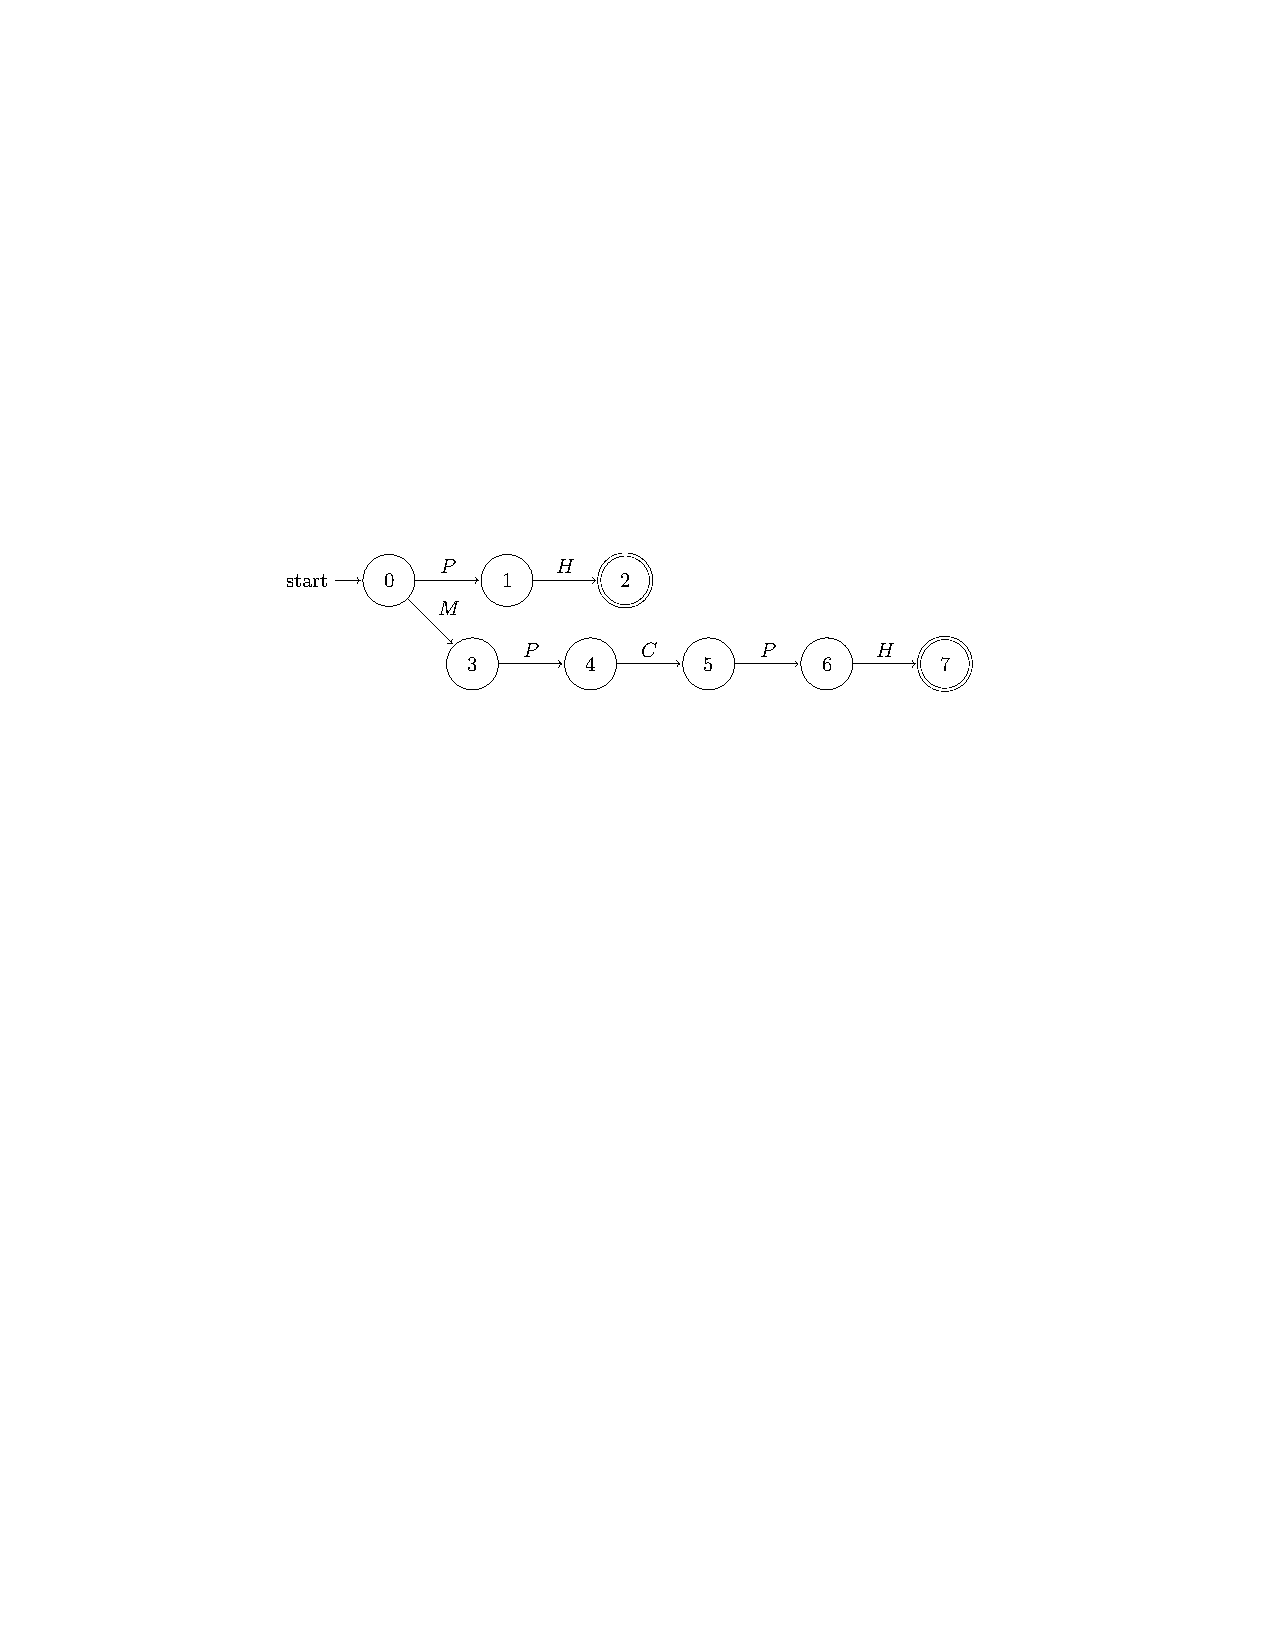
\includegraphics[width=\textwidth]{fig/original.pdf}        \caption{}
    \end{subfigure}%
    \begin{subfigure}[b]{0.3\textwidth}
        \centering
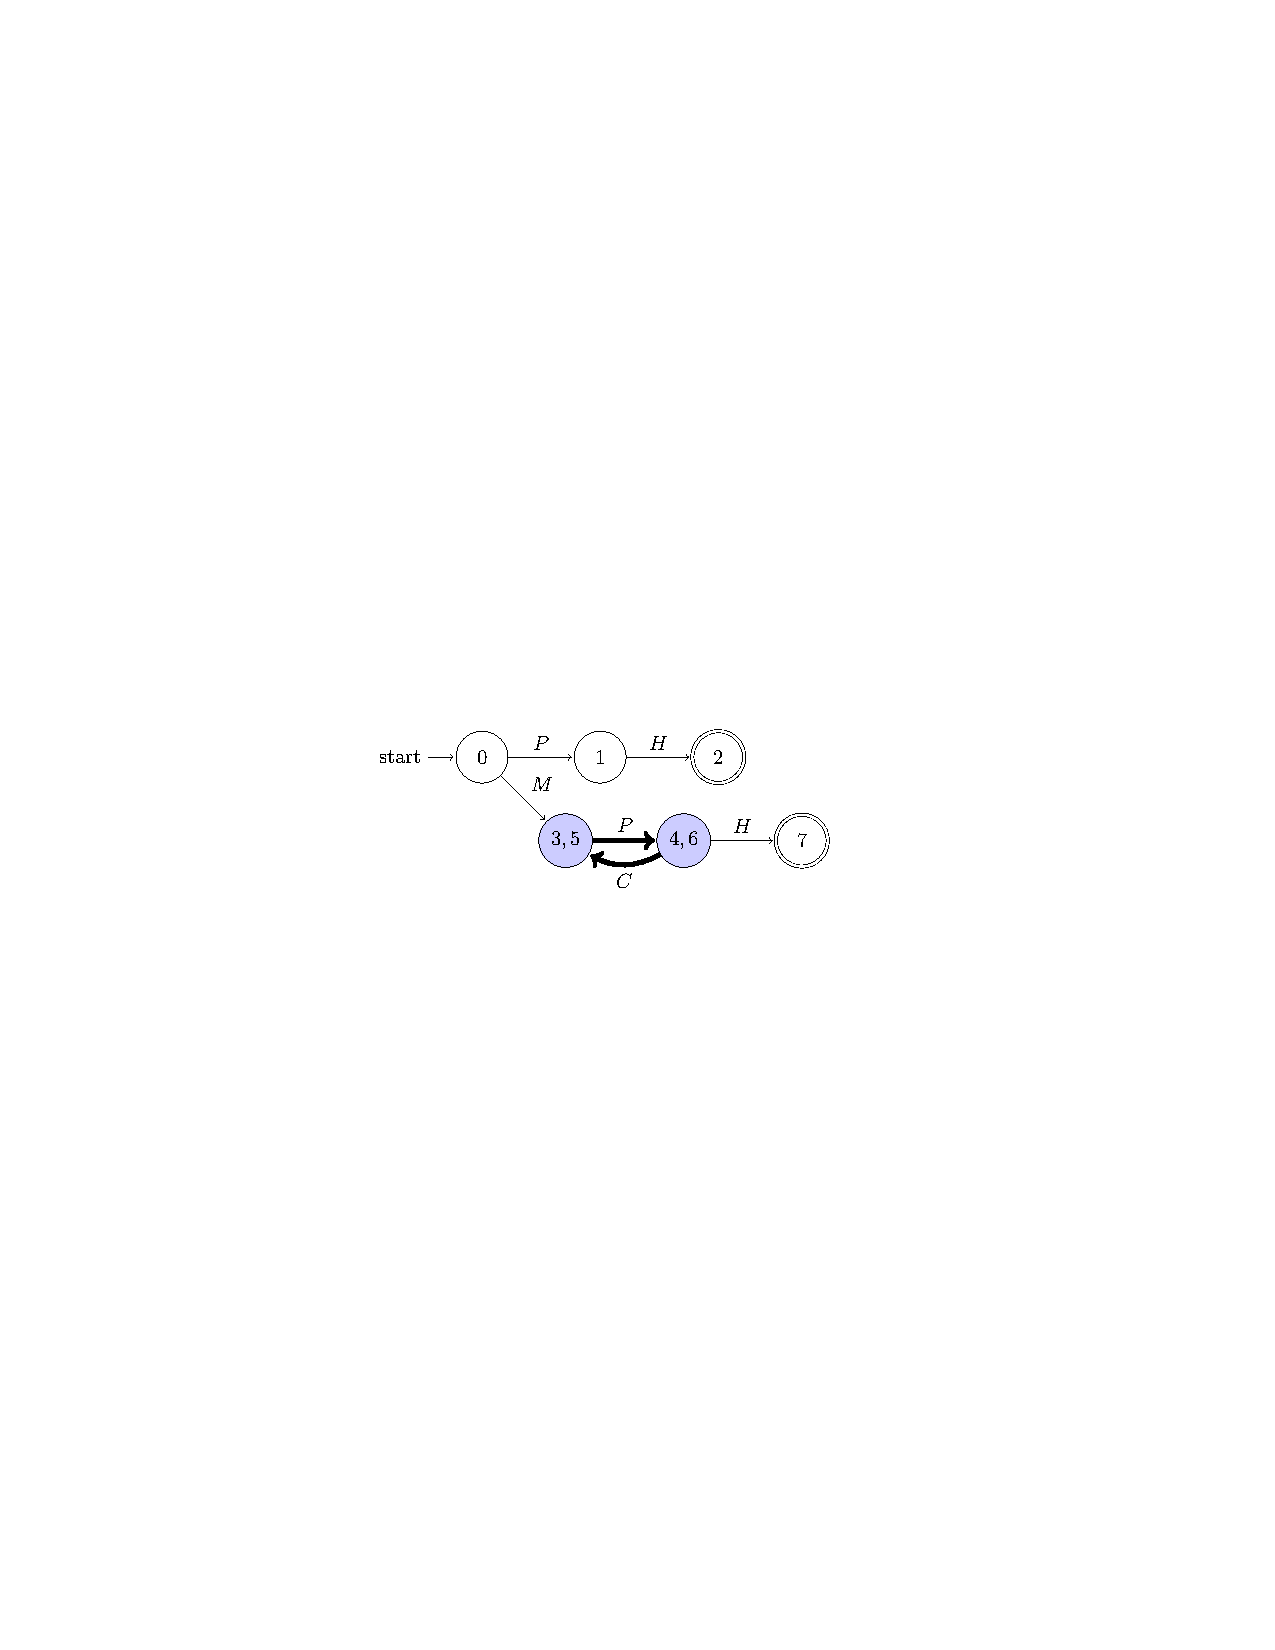
\includegraphics[width=\textwidth]{fig/merge1.pdf}         \caption{}
    \end{subfigure}%
    \begin{subfigure}[b]{0.28\textwidth}
        \centering
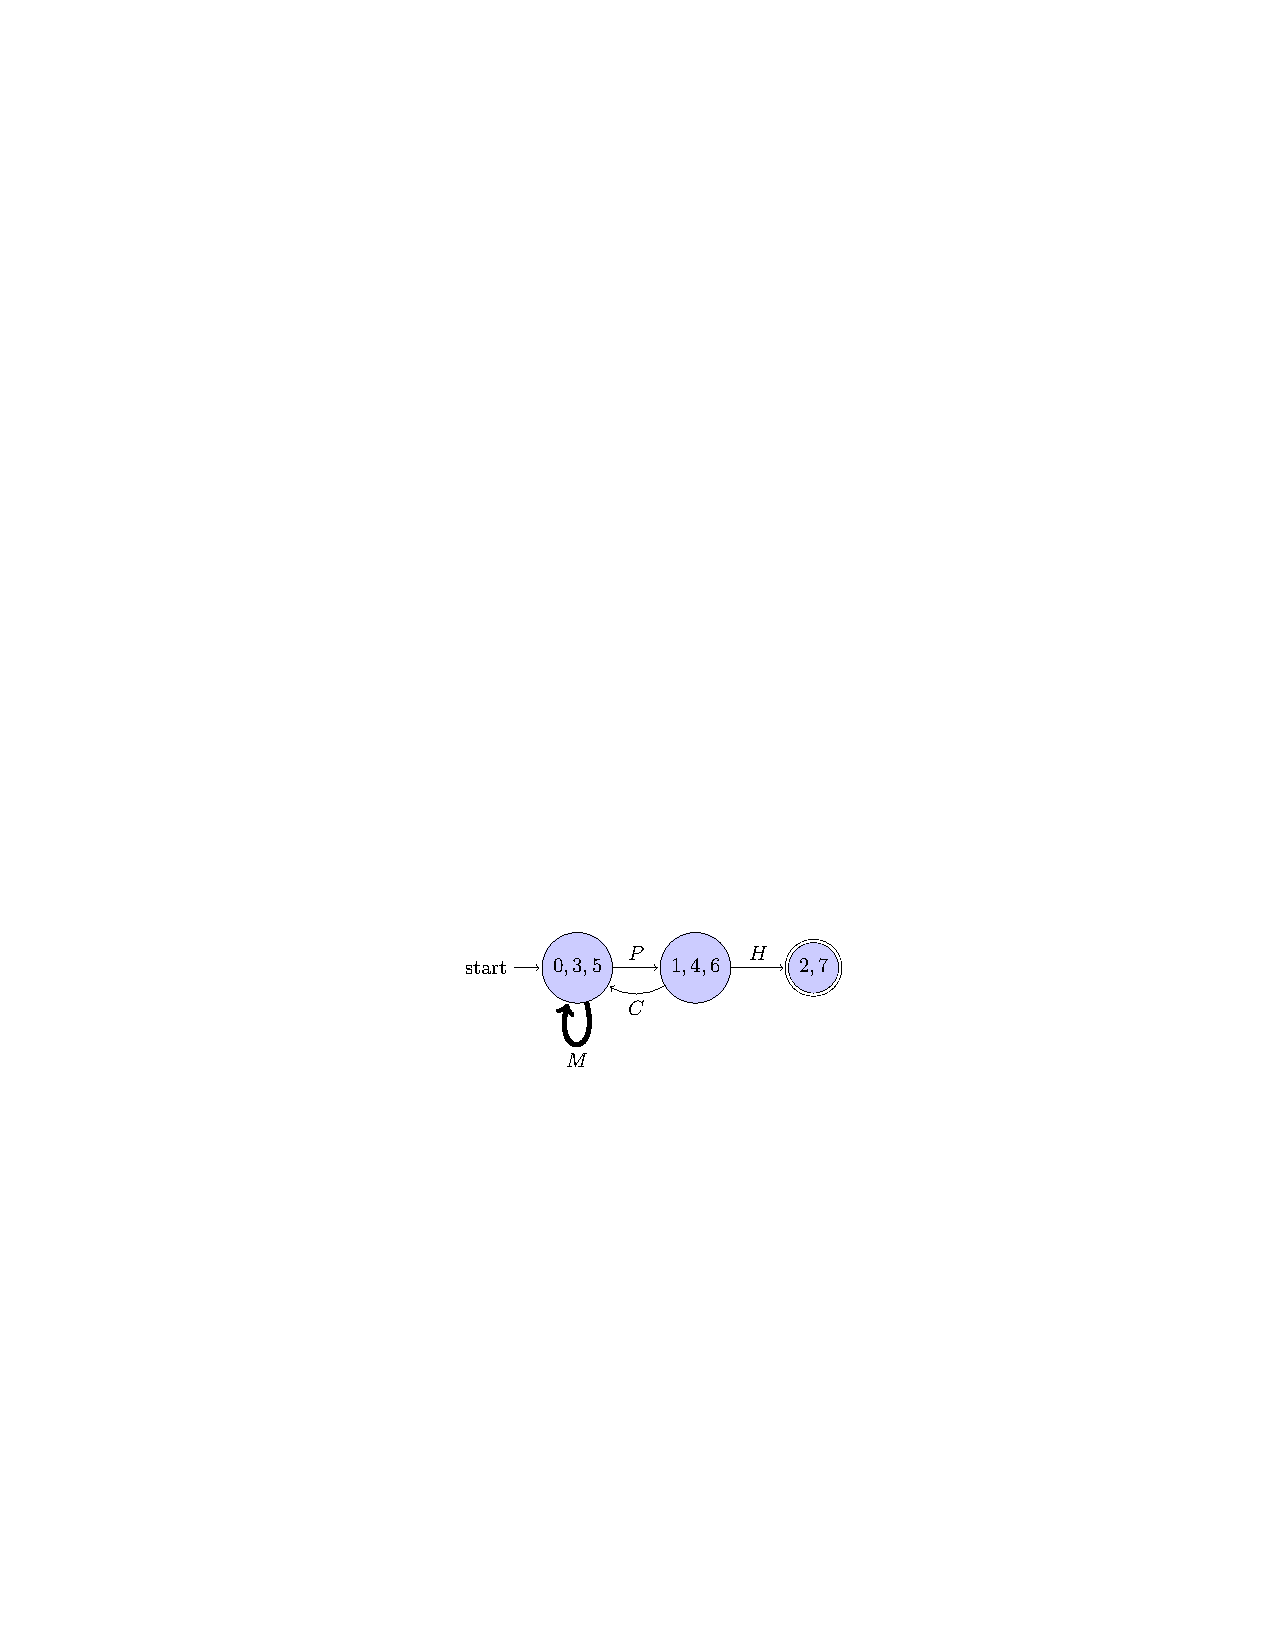
\includegraphics[width=\textwidth]{fig/merge2.pdf}     
\caption{}\end{subfigure}
    \caption{An illustration of grammatical inference algorithm using state merging. (a) is the original prefix tree/skill tree. (b) generalizes (a) by merging state $3,5$ and $4,6$. (c) further generalizes (b) by merging $0,3,5$, $1,4,6$, and $2,7$. The state merging or splitting is guided by a GI algorithm selected for the target language on positive data only, or with both positive and negative data.}
    \label{fig:gi}
\end{figure}


In this specific application context, we will consider several GI algorithms, such as \cite{heinz2013learning} for learning from positive demonstration under the assumption that actions have pairwise dependence, and the $L^\ast$ algorithm, which learns from both positive and negative demonstrations \cite{angluin1987learning}, given that negative demonstrations may be obtained from the nurses’ feedback of unreasonable behaviour. We propose to learn, for three interacting agents, their individual alphabets and languages. We seperate the concern of  action synchronization, conflict, and sequencing from learning and propose to capture such constraints for collaboration and coordination through product operations between languages/automata, including but not limited to, synchronization composition and sequential composition \cite{alur2015principles,hopcroft2001introduction}. 
For instance, synchronization will enable us to capture the dependency between the action of aiming the camera at the hand of the human nurse with the reaching motion for the manipulator.  Inference algorithms for probabilistic finite-state automata \cite{clark2004pac} \cite[Chap 12]{de2010grammatical} will further enable us to capture stochastic transitions resulted from uncertainty outcome of actions and uncertainty in task step coordination. 

\paragraph*{Learning shared object affordances:}
%When human and robot cooperatively manipulate a shared object, we will use the knowledge of shared affordance  to determine if human and robot actions are compatible. 
Object affordances define the operations that an object can afford a human/robot operator to perform~\cite{gibson2014ecological}. By learning these affordances, we aim to establish the relation between the consistent changes of the object states and the robot’s action sets. As high-level task knowledge, object affordances not only enable the object to be categorized by their functions, but also correlate a robot's general low-level motor skills with specific task contexts~\cite{fitzpatrick2003learning, veloso2005learning, thomaz2009learning,lopes2007affordance,montesano2008learning, lopes2010abstraction, kjellstrom2011visual,aksoy2011learning}. Research efforts thus far have investigated the affordance of a object manipulated by a single operator. Yet, it is still unclear in cooperative manipulation tasks, given operations the human and robot partners can apply to the shared object, what will be the appropriate task sharing. For example, when a human nurse and a nursing robot collaboratively remove a dirty blanket from a patient, given the position where the human nurse has grasped the blanket, the robot needs grasp the other corners so that the blanket will not be dragged away but will be lifted and removed instead. Although the blanket affords grasping at any point, as a shared object in cooperative manipulation, the robot operation it can afford is determined by the applied human operation. 

To represent the knowledge of shared object affordances, we will create a hierarchical object affordance library that categorizes objects by their functions and associates the constraints on the object states during the cooperative manipulation (e.g., lift the food tray in balance) 
to objects in the same sub-category. We will then use these constraints to evaluate if the applied joint action of human and robot are compatible. For instance, when a human nurse and tele-nursing robot collaboratively move a patient transfer bed, or a human nurse hands over a medical tool to robot the shared object affordance will inform the robot where to grasp given the observed human partner's grasping positions.
% \todo{JF: Is there other form of shared object? two mentioned two examples are similar.}

%-------------------------------------------------------------------------
\subsubsection{Activity 1.3 --- Fast adaptation of motor skills to personalized user needs}\label{sec:plan-motion-high}
%-------------------------------------------------------------------------
Through low-level and high-level learning, we shall construct the motion intelligence of the mediating robot that consists of general task knowledge and general motor skills. Here we further propose to %framework that 
employ the robot's motion intelligence for fast adaptation to the personalized needs of human users. Our key idea is built on a two-level motion knowledge: A robot's motion intelligence should be equipped with computational models for \textbf{General Motion Templates}---the motion knowledge hierarchy from the low-level motion templates to the high-level motion plans; \textbf{Special Skills}---the highly customized motor skills that address a user's particular needs in the activities of living and workplace. The two aspects of motion knowledge differ in their generality and thus require different strategies for acquirement, maintenance, and refinement. To this end, we propose a lifelong learning and adaptation method to integrate knowledge-based motion control and online data-driven motion adaptation seamlessly. This method will allow the system to continuously improve its motion intelligence without the burden of maintaining a large database and increased local computational efforts. 


To illustrate our proposed method, consider a nursing robot learning collaborative manipulation for a new object from robot-mediated interaction. Before being deployed to the new task, the robot has been trained off-line and acquired general motor skills for manipulation, such as coordinated reaching and grasping. Using large and general demonstration dataset, the offline training can derive robust computational models for the robot end-effector's reaching motion primitives and frequently grasping hand pre-shapes (i.e., the general motion templates). However, the offline training is not informed of the personalized and/or task-specific needs. For example, in collaborative nursing tasks, the robot should render  arm postures that are natural and accommodating to its collaborating human nurse. At the same time, by observing the teleoperator in a new task, the robot will be notice that compared to the reaching motion primitives it has, the movement primitives extracted from the new demonstrations are significantly different at the degree of freedom that measures the arm posture (i.e., the rotation of the elbow with respect to the should-wrist axis, namely the swivel angle~\cite{Tolani_Badler:96}), but are quite similar at the degrees of freedom for end-effector trajectories. Given the similarity and difference, the robot will propose to the teleoperator to perform incremental learning to update motion primitive models for the end-effector trajectories~\cite{havoutis2016online}. To be specific, we use DP-means~\cite{kulis2011revisiting} --- an online GMM building algorithm --- to incrementally update the GMM/GMR model generalized over multiple off-line demonstrations, based on the the squared Euclidean distance from the new data to the GMM cluster centers. Base on the same idea, we can also perform decremental learning to forget obsolete demonstrations. However, the motion template for swivel angle trajectory must be overwritten by the special skill in the specific tasks (after confirming with the expert teleoperator), if the new demonstration and general motion template have significantly different DMP models. By observing how the teleoperator chooses to adjust a pre-defined hand pre-shape to grasp and manipulate a new object, our proposed framework also creates models for Special Skills such as the correlation between the hand pre-shape and new objects.  

% \todo{JF: need some detail about incremental learning, the reference \cite{hewitt2017dmp} does not seem to address this.}

%  From a system abstraction viewpoint, the set of high-level tasks that can be achieved jointly by the teleoperation system, the human nurse, and the patient, can be understood as a \emph{language} $L$ over the \emph{alphabet} $\Sigma$. Each symbol in the alphabet corresponds to a low-level closed-loop controller with certain parameters. For example, approaching a desired goal position is achieved with a navigation control parameterized by a goal position and velocity, while picking an object is parameterized by the object affordance, force control, and object position. With the low-level parameterizable control actions, i.e., alphabet, a high-level feasible task becomes a \emph{sentence composed of symbols with appropriate parameterization}. For example, the concatenation of go to the table ($a(p_1)$) and pick up the cup on the table $b(p_2)$ is only possible if the goal position $p_1$ makes the cup within the reachable workspace of the manipulator. This is similar to pre- and post- conditions of actions in situation calculus \cite{}, except that we now use parameterized actions to enable generalization and flexible reusing of the low-level controller. Building with parameterized actions, we construct symbolic models of a dynamic system with methods \cite{fu2013bottom}. For time-invariant systems, the symbolic model can be represented as an automaton, which is a representation of a language.

%Our goal is to achieve high-level task learning and reasoning by integrating this abstraction-based control synthesis for hybrid systems with abstraction-based learning from demonstrations.





% In addition, we also consider the approach of constructing skill tree~\cite{konidaris2012robot} and extend this concept to \textbf{shared skill tree} to encompass the robot-mediated collaboration scenario.  In the framework of shared skill tree, we will integrate the idea of high-level symbolic representations to model the tree component that involves complex collaboration~\cite{konidaris2018skills}. This method abstracts actions and states as symbols and therefore formulates a complex planning task to set and propositional operations. To adapt to the robot-mediated collaboration scenario, we revise the framework in~\cite{konidaris2018skills} by associating the symbolic representation of actions and states to their human/robot owner, so that the high-level task representation can be more inclusive and flexible. 







% and space of possible collaborative task decompositions from the interactions between human end users and a teleoperated nursing robot. To illustrate collaborative task decomposition, consider two typical scenarios for collaborative tasks: 

% \begin{itemize}
% \item {\it A task without a shared object}: For a task that consists of multiple sequential/parallel subtasks, human and robot are responsible for different subtasks but do not interfere with each other. Although they do not cooperatively manipulate any shared object, they affect each other's action and performance because (1) the step completed by the robot must precede the actions of its human partner and (2) the effectiveness of the robot at its current subtask %step (measured in terms of accumulated reward) 
% will influences its partner's efficiency in the next subtask. %cause its partner to improve, maintain, or decrease performance in the next step. 
% In this case, the collaborative task decomposition will define which subtasks are assigned to the human and robot by matching their physical capabilities to the task affordance. Particularly, for the steps that the robot is responsible for, it defines the acceptable range of final states. % and/or acceptable performance measured by accumulative reward in the collaboration.  

% \item {\it A task with a shared object}: For some subtasks, the human and robot cooperatively manipulate a shared object. In this case, the collaborative task decomposition specifies which part of the object is possible for the human/robot to manipulate given the object affordance, in addition to possible subtask role assignments and acceptable final states. % and task performance. 
% For instance, for the task that human nurse and nursing robot cooperatively manipulate a patient transfer bed, where the robot can grasp and push the bed depends on where the human nurse grasps and pushes, and vise versa. As the shared object involved, the temporal and spatial motion coordination between human and robot becomes more critical. It is also important to extend the concept of individual object affordance to shared object affordance and define their affordable operation in abstract representation. 

% \end{itemize}

% % \paragraph*{Abstraction-based control and learning}
% \paragraph*{Learning abstract representations of collaborative task decompositions}
% % \zhi{this can be used to learn high-level collaborative task decomposition}
% % To learn from the robot-mediated interaction, explicit learning and programming each task sequence is not only time consuming but also inflexible given any changing environment, e.g. different patient needs, changed operating rooms, cooperated nurses.
% We consider multiple approaches for learning the abstract representation of collaborative task decompositions. Our first approach is 
 
% \jie{It is a bit lengthy and tedius, I put it here for now but we will see if it is truly needed.}
 
%  We seperate the concern of low-level learning and describe later a statistical model will be used to capture low-level parameterization—similar to goal-directed intent— due to the inherent nondeterministic decision making or behavior uncertainty of humans. Instead of positioning at a specific pose, statistical methods will learn a distribution of possible poses for manipulation tasks using intention-aware planning \cite{bandyopadhyay2013intention}, where the goal of manipulation is treated as a hidden parameter and can be inferred from the demonstration using Bayesian reasoning.



% The high-level learner abstracts away low-level parameter but focuses only on the behavior coordination and task decomposition level. Next, we propose methods for low-level learning of parameterized actions. 
%  to (1) use high-level symbolic representation for task modeling at high-level, 


% present CST, an online algorithm for constructing
% skill trees from demonstration trajectories. CST segments a demonstration trajectory
% into a chain of component skills, where each skill has a goal and is assigned a suitable abstraction
% from an abstraction library. ese properties permit skills to be improved efficiently using a policy
% learning algorithm. Chains from multiple demonstration trajectories are merged into a skill tree.

% \zhi{I will also add GEorge Konidaris' method of Constructing Skill Trees by Demonstration, and extend his framework to shared skill tree that consist of the skills of on-site human nurse and the skills of robots --- this could be an alternative method for learning collaborative task decomposition; Also refer to his work on Learning Symbolic Representations for Abstract High-Level Planning }




% \paragraph*{Shared autonomy through Task-specific generalization:}
% Intelligent task affordance learning should not only reproduce expert demonstrations for the set of training tasks but also generalize to achieve good performance for tasks that have never been encountered before. At low-level motion described by DMP, action generalization methods has been developped in \cite{ude2010task}. The method generalizes from a set of DMP parameters, each of which is for  a specific configuration, to a function $f: q \mapsto (w, \tau, g)$   that maps from the continuous configuration space to the continuous DMP parameter space (linear parameter, phase, and goal). We propose a two-tier approach to combine task-specific DMP generalization with goal inference and task affordance learning to develop guided assistance for novice teleoperator. The approach decouples motion guidance from task guidance: Task guidance directly relates to task affordance learning and aims to  guide the novice user step by step in completing a specific dynamic task with sequential composition of local subtasks. Motion guidance aims to generate guiding force via haptic devices so that the user can be assisted to achieve motions that requires dexterous manipulations, such as reaching in cluttered environment, reaching and grasp with autonomous object affordance reasoning for the best grasp.

% During the cooperative manipulation, the robot keeps monitoring the trajectories of the object's manipulation-related states,  


% , and (2) the set of motion primitives that model the  trajectories of the object's manipulation-related states during their cooperation

% Under shared-autonomous control, if the supervisory teleoperator notice 





% the model the temporal and spatial correlation between human/robot hands with respect to each other, and with respect to the moving center of the blanket.  

% \zhi{(1) Learning functional object affordance; (2) Learning shared object affordance from collaborative manipulation} 



% \textit{\textit{\jie{goal-directed learning shall be coupled with inverse reinforcement learning to capture not only the goal, but how the human operator achieves the goal.}

% \jie{Possible subtasks based on discussion: Jane suggested skill tree learning and low-level DMP learning. Propose to use shared intent inference} 

% \zhi{Learning the coordination of mobile base with manipulation --- as far as the reward function concerned, here are several coordination policy hypothesis: manipulability, reachability, vision advantage (perception convenience and comfort); minimal intervention of macro-structure (also relevent to energy consumption); environment constraints (static obstacle, prediction of moving obstacle and agents)}
% }}

% \paragraph*{Share intent inference}

% * What is the problem?

% * Formulation (mathematical)

% * proposed approaches (at least two): 


% \paragraph*{Problem Formulation}
% * Task 1 - Learning physical interaction with nurse and with patient 

% 	* Demo 1 - Human nurse hand-over object to patient

% 		* Learning object/task affordance
% 		* Learning the phase matching in human-human interaction
% 		* Learning how the human nurse adapt to the patients with limited motor capability 
% 	* Demo 2 - Expert teleoperator and human nurse perform robot-mediated collaborative task

% 		* Human nurse leads the task
% 		* Learning from teleoperator's responsive motion to the end user 
% 		* Robot controlled by the teleoperator can learn from the teleoperator the feasible and appropriate operation given the robot's limited physical capability and teleoperation transparency
% 		* Teleoperator can communicate with human nurse on-site tof negotiate via bidirectional telepresence

% 			* Teleoperator who can not precisely perceive the spatial and temporal information of the task from inconvenient and/or insufficient camera view
% 			* The teleoperator can receive feedback in terms of verbal critique and gestures from the end user
% 			* The bilateral communication between teleoperator and end user can compensate the lack of information and correct the motion errors due to mis-perception


 



% Similar to the fast adaption of low-level motor skill, our framework can also update the high-level collaborative task affordance, including the 


% Building upon these results, it is possible to develop a self-evolving motion intelligence, which can \textbf{acquire} user-specific and customized motor skills based hierarchical motion knowledge and generalized skill sets, can \textbf{reflect} upon its motion knowledge hierarchy to refine its motor skills and improve its learning efficiency.   



%   which can customize the general motor skills of the 

% incremental and decremental learning

%-------------------------------------------------------------------------
\subsection{Activity 2 --- Fast intention forecasting and blended control for robotic mediation}\label{sec:plan-intent}
%-------------------------------------------------------------------------
\noindent
{\bf Problem statement:} For interactions between humans and robots in nursing tasks, shared intent is the key to successful collaboration \cite{cite}.
Thus, the robot must be able to infer the intentions of nurses, teleoperators, and patients, at both the level of motion primitives and at the level of task decompositions and assignments to appropriately mediate the joint task through shared autonomy. In this activity, we propose to leverage the knowledge and models we constructed in Activity 1 to provide: (1) shared intent forecasting of high-level tasks, sub-tasks, and role assignments within a cooperative game formulation; and (2) intent forecasting of subtasks from motion primitives through robot mediated demonstrations.  We then use these intention forecasts to enable: (1) autonomous control of the robot's navigation based on teleoperated control of manipulation; and (2) assistive teleoperated manipulation based on intent forecasting and task knowledge.
%Here, we focus on novice teleoperators and relax the strong coordination and near optimality assumptions employed to learn from expert teleoperators in Activity 1.

\noindent
{\bf Probabilistic approach:}
Following existing probabilistic reasoning methods for intent \cite{wang2013probabilistic},
we estimate intended tasks, denoted as ``language'' L, from a partial sequence of subtasks, denoted as ``states'' $s_{1:t}$ and the (partial) motion primitive(s), denoted as controls $u_{t+1}$, currently being executed by each participant using Bayes theorem and hierarchical/Markovian properties:
\begin{align}
& P(L|u_{t+1}, s_{1:t}) \propto \sum_{s_{t+1:T}} P(u_{t+1}|s_{t+1}) P(s_{1:T}|L) P(L); \label{eq:forecast}\\
& P(s_{t+1}|u_{t+1}, s_{1:t}) =
\sum_{L}\sum_{s_{t+2:T}} P(s_{t+1:T}|s_t,L) P(L|u_{t+1}, s_{1:t}).
\end{align}
Key quantities for estimating these low-level sub-tasks and high-level tasks are 
the likelihoods for the high-level task decomposition and assignment, $P(s_{1:T}|D)$ and
(partial) motion primitives under different subtasks, $P(u|s)$.  We discuss models for each of these in the following sections.

%-------------------------------------------------------------------------
\subsubsection{Activity 2.1 --- Inverse Reinforcement Learning for Task Decomposition and Role Assignment}\label{sec:plan-intent-Stackelberg}
%-------------------------------------------------------------------------

% \todo{Jane: Given the high-level task structure learned in Activity 1.2, activity 2.1 uses Stackelberg Game Formulation to infer the collaborative task assignments between expert teleoperator and an on-site human nurse. The demonstration task can be human and robot collaboratively organize and clean the patient room. For such a task, activity 2.1 will provide a reward function to optimize the task allocation, particularly for the subtask that both robot and human nurse can do -- such as who is going to pick which object, and who is going to fetch a far-away object --- to optimize task efficiency and accommodate human nurse's preference. }

\noindent
{\bf Problem Formulation:} Using the space of task decompositions for a given task defined by language $L$ in Activity 1.2, we seek to learn the preferred decomposition and the assignment of the human partner and robot to the sub-tasks of the decomposition.  To support probabilistic reasoning in Eq. \eqref{eq:forecast}, we construct a probabilistic model of sub-tasks for the given task, $P(s_{1:T}|L)$, where $s_t$ represents both the sub-task and role assignment of each participant (e.g., robot, nurse, or patient) at subtask step $t$.

\noindent
{\bf Cooperative Stackelberg Game Formulation:} 
The nature of collaboration leads us to consider the problem of coordinating behavior using game-theoretic formulations: In this game, two agents collaborately perform some mutually desired task. The observed demonstrations, including the demonstrations of the robots and those of the nurse, result as a solution of the cooperative game in which both agents act jointly to maximize a performance criteria expressed as a reward function $R: S_{t,1} \times S_{t,2} \times S_{t+1,1}\times S_{t+1,2} \rightarrow \mathbb{R}$ where $S_t$ and $S_{t+1}$ are consecutive sub-tasks is the world state of two collaborators (e.g., the robot and the nurse) and can sometimes be a shared cooperative sub-task, as shown, or factored as $R_1 + R_2$ with $R_i: S_{t,i} \times S_{t+1,i} \rightarrow \mathbb{R}$.

We employ an important simplifying assumption---that the human partner takes a lead role and sub-task selection is coordinated to be consecutive.  This is based on observations that 
hierarchy and role assignment are often observed in collaborative human teams \cite{mortl2012role,colman2014explaining}. For example, a human nurse may take the leader role and guide the tele-operated robot
%, or the teleoperator indeed,  
towards the goal position when they collaboratively transport a patient bed. Thus, it is meaningful to consider a class of hierarchical game, called cooperative Stackelberg game \cite{basar1999dynamic}, to capture the selection of the particular task decomposition and assignment of roles to subtasks selected by the collaborative pair.

\noindent 
{\bf Centralized Maximum Entropy Inverse Reinforcement Learning for Cooperative Tasks:} We propose to extend inverse reinforcement learning methods \cite{ziebart2008maximum} to learn utilities for the selection of a specific task decomposition and assignment of its subtasks in the sequential turn-taking order of the Stackelberg game representation. These learned utilities are estimated to rationalize coordinated behaviors that have been demonstrated.  
However, our approach can be viewed as ``centralized'' in the sense that each player's conditional probability distribution is not separately modeled.
Following the Stackelberg game representation, we define utilities in terms of the current state and joint actions from all agents. These will often be independent sums of each agent's individual utility when employing independent motion primitives or sensory motion primitives. 
We consider maximum entropy inverse reinforcement learning \cite{ziebart2008maximum} generalized to use minimum relative entropy with respect to a reference policy $P_0$.
Under this formulation, a particular task decomposition and assignment $s_{1:T}$  from language $L$ with reward $R(s_t,s_{t+1})$ is predicted with probability $\prod_{t=1}^{T-1} P_0(s_{t+1}|s_t) e^{\sum_{t=1}^T R(s_t,s_{t+1})}/Z$, where $Z$ is a normalization term over the entire language and possible assignments: $Z = \sum_{s'_{1:T}\in L} \prod_{t=1}^{T-1} P_0(s'_{t+1}|s'_t) \sum_{t=1}^T e^{\sum_{t=1}^{T-1} R(s'_t,s'_{t+1})}$. This term can be difficult to compute exactly since the language $L$ is often not finite.

\begin{wrapfigure}{r}{0.4\textwidth}
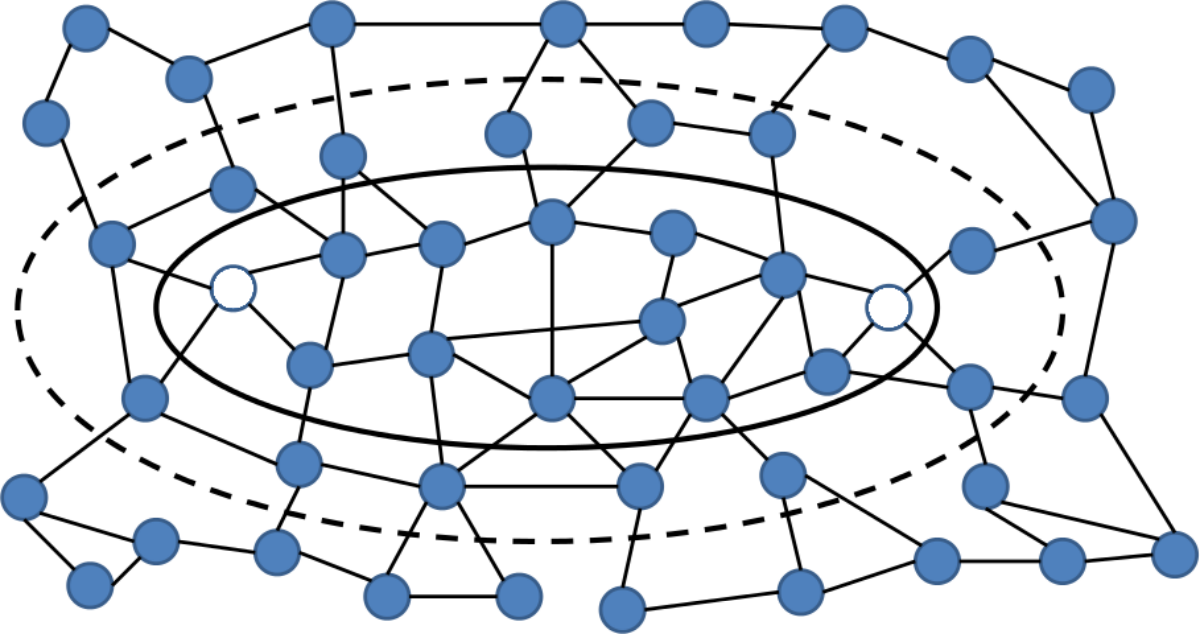
\includegraphics[width=0.4\textwidth]{fig//softstar.png}
\caption{Simple illustration of the heuristic-guided search approach to approximate probability estimation between two endpoints (white states).  The set of states in the solid black oval are active. The additional ones inside the dotted oval are on the fringe.}
\label{fig:softstar}
\end{wrapfigure}

We propose to extend heuristic-guided methods for single-agent maximum entropy inverse reinforcement learning \cite{monfort2015softstar} to this cooperative multi-agent setting.
The key idea is to uncover a subset of the state-space of language $L$ that captured most of the probability mass for computing $Z$.
This is illustrated in Figure \ref{fig:softstar}. Upper bounds (heuristics) for the contribution of sequences through states in the fringe are used to incrementally expand the active set of states (black oval) and bound the overall approximation.
Cooperative tasks, though often incorporating large state effective spaces (based on language $L$), have some distinct advantages for this approximation scheme.
First, much of the tasks is often broken down into individually-executed sub-tasks; the ``probability mass'' of these can be computed independently and then integrated into the overall estimate;
Second, heuristics can be naturally obtained by making relaxations to some of the participants constraints; for example, assuming that the collaborative partner is able to optimally assist with every sub-task defies constraints for the adversary, but provides a useful heuristic.
Third, so long as the reference policy $P_0 < 1$ and some regularization of the estimated rewards is imposed, the entropy of the resulting distribution must be finite, which avoids the tendency of standard maximum entropy IRL towards a uniform distribution over trajectories---typically with infinite expected length \cite{ziebart2010modeling}.

% \subsubsection{Activity 2.1: Forecasting the intent of motion primitives from robot-mediated demonstrations} 
% %In this subtask, we examine the question: Is it possible to infer tele-operator's intent from the robot mediated demonstrations? The purpose of inferring teleoperator's intent has two-fold: On one hand,
% An understanding of motion primitive intent can enable the robot to use blended control \cite{downey2016blending} to ease the effort required from a novice teleoperator to achieve the control objective. For example, in a task of rearranging utensils on a table, with the ideal blending control, the teleoperator maintains control of high-level movements, such as moving the hand towards the cup (\emph{intent}) and when to grasp (\emph{intent}), while the autonomous robot handles the details of this task and performs intuitive, human-like motion using DMPs. This is only possible if the robot knows which object the user intends to pick up. 

% %On the other hand, for the purpose of training novice teleoperators, if we obtain imperfect tele-operation demonstrations, how to infer the underlying intent and aid the novice user? \jie{I think it is important. However, the current method cannot do this.}

% To answer this question, we formulate the problem in IRL setting: the tele-operator has an unknown reward function for which his behavior is assumed to be near optimal. The reward function captures goal-related reward and risk-averse behaviors, as well as other performance criteria such as efforts involved in operating the input devices. 
% The challenge is that in this IRL problem, we obtain two demonstrations simultaneously: One demonstration $d_h$ is given by the tele-operator using the input device and demonstration $d_r$ is given by the tele-nursing robot. The mapping from $d_h$ to $d_r$ is in general a nonlinear function internalized by the expert. If we simply seperate the demonstrations into $D_h$ and $D_r$, and apply IRL to solve two separate reward functions, we remove the coupling between the reward functions and the unknown mapping. Another approach is to consider a joint reward function $R$ defined over the product state space between the workspace of tele-operator and the workspace of the robot and use IRL algorithm to learn $R$. A potential problem with this approach is that it does not distinguish the performance criteria for tele-operation and the user's preference for tele-operation. To address this, we propose an approach inspired by planning in shared autonomous MDPs \cite{fu2016synthesis}: Consider there are two reward functions $R_h$ and $R_r$, defined over the product state space between the workspace of tele-operator and the workspace of the robot. The behavior of the tele-operated system can be viewed as if the system performs a Pareto-optimal policy that aims to balance maximizing $R_h$ (goal-reaching, smoothness, time-efficiency in tele-operation) and $R_r$ (goal-reaching, safety, efforts in robot maneuvers): A policy is Pareto optimal if there is no other policy that can make it better for one objective than this policy without performance degradation for another
% objective. Thus, the IRL problem needs to solve (1) reward functions $R_h$ and $R_r$, and (2) a pre-defined weight vector $w_h, w_r$ that pinpoint on solution from the Pareto optimal set. Our approach is illustrated in Fig.~\ref{fig:pareto_irl}, where for a given set of weights, we employ the Chebyshev scalarization method \cite{perny2010finding} to find Pareto-optimal policies. In addition to reward inference, the inference of weights will be treated as a hyperparameter optimization problem using the primal and dual formulation of maximum likelihood estimation in IRL setting \cite{franceschi2017forward}.
% \begin{wrapfigure}{r}{0.6\textwidth}
%   \begin{center}
%     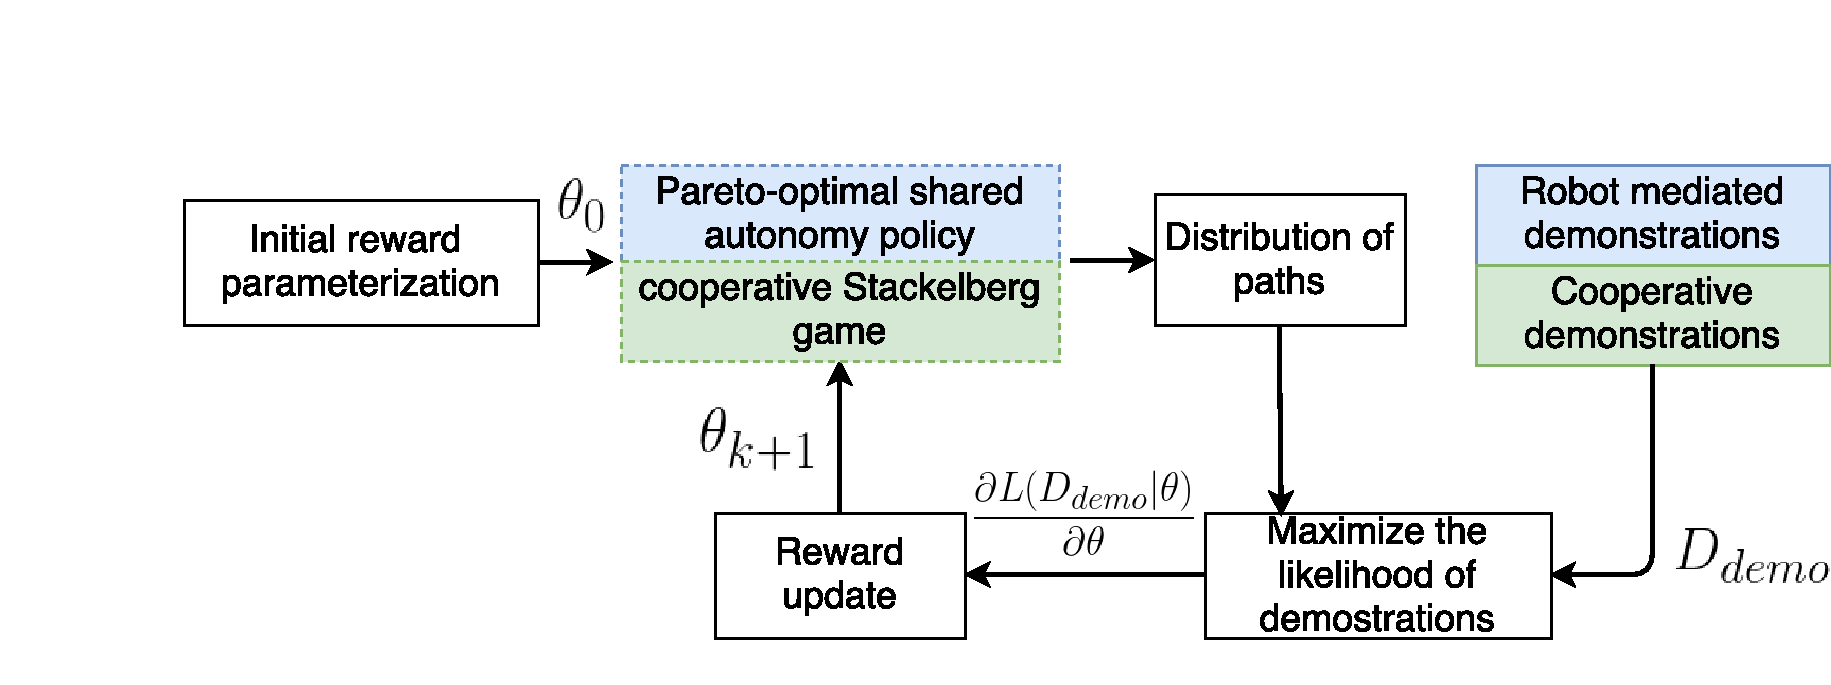
\includegraphics[width=0.58\textwidth]{fig/IRL_game1}
%   \end{center}
%   \caption{A block diagram showing the proposed IRL algorithm for intent inference for (1) teleoperator's intent through robot mediated demonstrations (Blue) (2) shared intent between teleoperator and end users for cooperative tasks (Green). Note in (1), the parameters $\theta$ includes a tuple $\theta_h, \theta_r$. }
%   \label{fig:pareto_irl}
% \end{wrapfigure}
% \jie{This figure can be edited here: \url{https://goo.gl/hkyinA}}

% The seperation of two rewards allows us to further consider personalizable tele-operation, as human individual may have different preferences on how to use the input device, characterized by $R_h$, but share a common knowledge on how the robot shall behave, given by $R_r$. Learning $R_h$ will help us to understand how to improve end user's experience. Most importantly it is possible to learn $R_h$ from simulated experiments. \jie{Jane: I am not sure if it is correct. still think about it.}

% \paragraph*{Intent prediction for coordinated tasks with end-users} In this subtask, we focus on the problem of infer the shared intention between human nurse and expert teleoperator. By inferring shared intention, the robot will be equipped with knowledge of how to coordinate its actions or motion plans based on the observed behavior of human nurses. This intent inference largely differs from existing IRL methods: Instead of answering ``what and how the demonstrator intents to do'', the robot aims to answer ``what shall we do together as a team'', by observing a partial demonstration from its interacting human nurse. 

% Is it possible to infer the shared intent, represented by the team reward function $R$, from demonstrations $\mathcal{D}$? Formulated as IRL problem, one possible approach is to substitute the solution by that of cooperative Markov game in Fig.~\ref{fig:pareto_irl}. However, cooperative Markov game with independent decision makers is difficult to solve  due to the coordination problem \cite{fulda2007predicting}. \todo{replace this ref if better one can be found.}

\paragraph*{Inverse Reinforcement Learning in Multi-Objective Decentralized Stackelberg Game}
The task assignments in collaborative teleoperated robot and
nurse team can be formulated as a Markov game $M=(S, A_1\times
A_2, P, R, F)$ where $S$ is a set of states, each including the joint
state of all agents and an auxierary task-related
state. The set $F\subseteq S$ is a set of \emph{task completion}
states: the task is completed only if a state in $F$ is reached. For
example, in collaborative pick-and-place of multiple utensils,
the task completion state is reached only when all objects are
collected.  The reward function $R$ specifies the \emph{unknown
end user's preference} of task completion, which determines a
policy for task assignment in collaboration. To ease the end
user's effort, the robot needs to infer user's preference and
assist the task completion. To this end, we propose the
stackelberg game formulation for IRL where the end user performs
the role of a leader and the robot performs the role of a
follower: When the end user decides his policy, he will safely
assume that the robot (follower) will pick a best response policy
in collaboration to the proposed leader policy. In parallel to the hierarchy in role assignments, this  by nature multi-objective: Maximizing the
end user's reward $R$ while ensuring overall (time or energy)
efficient task completion. Hence, we propose to incorporate
Pareto-optimal solutions in multi-objective cooperative
Stackelberg equilbrium: A policy is Pareto optimal if there is no
other policy that can make it better for one objective than this
policy without performance degradation for another objective.  Given that we know
the task completion reward, the IRL problem needs to solve (1)
reward functions $R$ that encodes the preference of the end user,
and (2) a pre-defined weight vector $w$ that pinpoint on solution
from the Pareto optimal set. We plan to extend our previous work on Pareto-optimal planning in Markov decision process for shared autonomy systems \cite{fu2016synthesis} to cooperative Stackelberg game for solving the inner problem in IRL. Further, to ensure a uniform spread of Pareto-optimal solutions given a uniform spread of weight vectors,  Chebyshev
scalarization scheme \cite{perny2010finding} will be introduced in solving  Pareto-optimal policies in multi-objective
cooperative Stackelberg game. The inference of weights will be posed as a hyperparameter optimization problem using the primal
and dual formulation of maximum likelihood estimation in IRL
setting. 
\begin{wrapfigure}{r}{0.6\textwidth}
  \begin{center}
    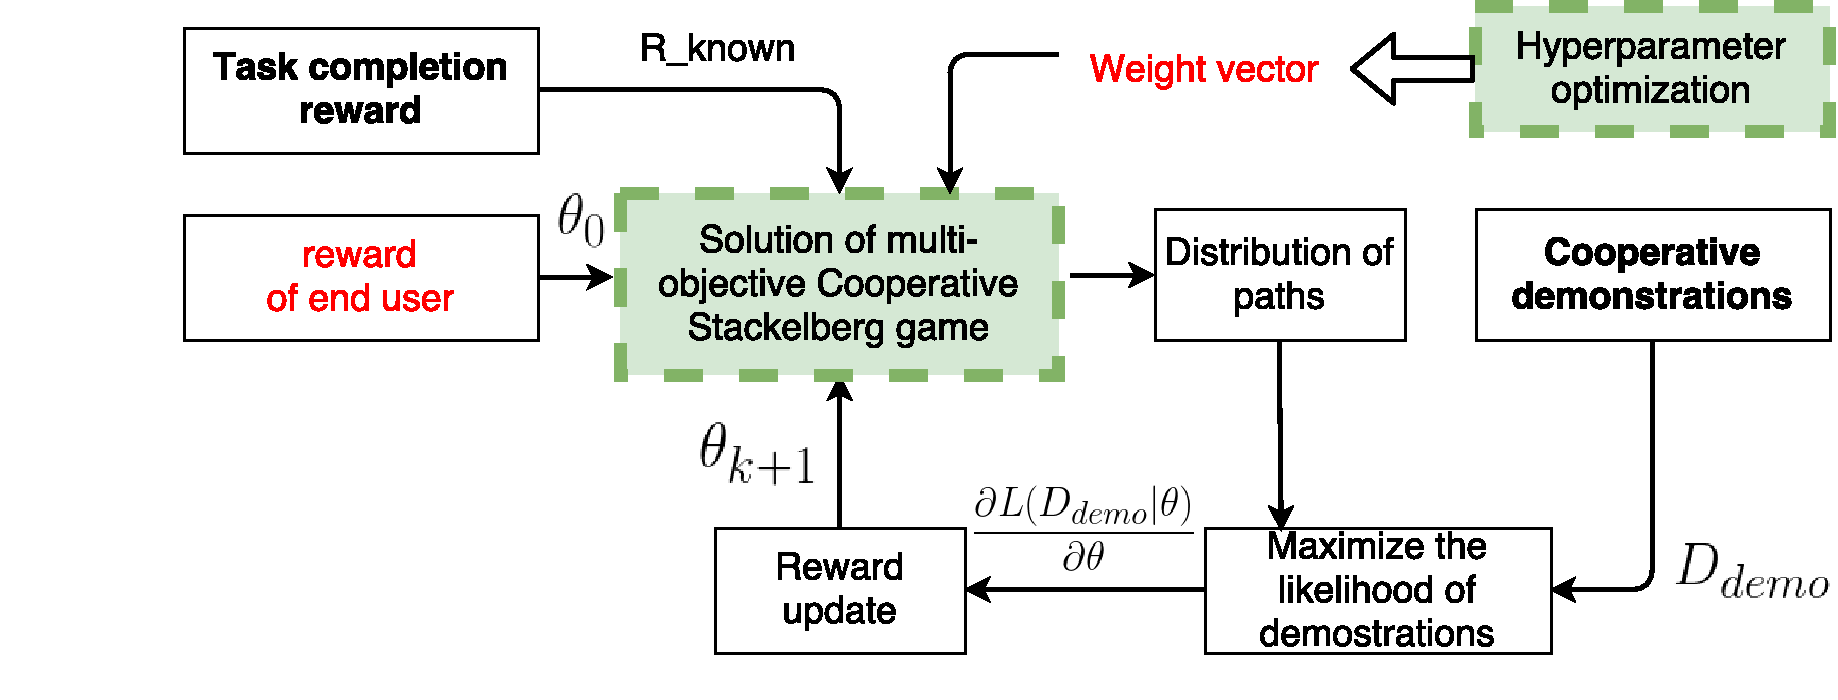
\includegraphics[width=0.58\textwidth]{fig/IRL_game}
  \end{center}
  \caption{A block diagram showing the proposed IRL algorithm for intent inference for  end users for collaborative task assignment. $\theta$ is the parameters in the unknown reward function. }
  \end{wrapfigure}

%-------------------------------------------------------------------------
\subsubsection{Activity 2.2 --- Recognizing Task Steps from Partial Motion Primitives}\label{sec:plan-intent-prediction}
%-------------------------------------------------------------------------

We now focus on recognizing the sub-task $s$ from a partial execution of the motion primitive $u$. To leverage this within our probabilistic formulation, in which it is a key component for forecasting low-level and high-level intentions, we estimate $P(u|s)$---the probability of the control sequence given the sub-task.

\paragraph{Similarity-based estimates:}

The first approach we consider is similarity-based estimates using exemplar motion trajectories.  For these, the similarity between a partially executed motion trajectory and a set of motion trajectories corresponding to different subtasks are evaluated and used to define the likelihood function.  The simplest of these is the Euclidean distance and a Gaussian distribution: $P(u|s) = e^{-\text{dist}(u_t,u_t^*(s)})$.
However, other distributions, such as the Laplacian distribution can also be employed.  Weightings for different components of the distance function (e.g., hand versus elbow position) can then be optimized to maximize the likelihood of correct associations.

\paragraph{Inverse reinforcement learning:}

Our second approach is based on the application of maximum entropy inverse reinforcement learning for linear-quadratic regulation problems \cite{ziebart2010modeling}.  Under this approach, a quadratic cost function ${\bf C}_s$ is learned that penalizes the state-control vector at each point in time, yielding a distribution: $P(u|s) \propto \exp{\sum_{t=1}^T [u_t \; s_t] {\bf C}_s [u_t \; s_t]^T}$.  Using our previously developed system \cite{monfort2015intent,schultz2017goal}, we will train this model from goal-directed teleoperation and provide prediction of the task step (i.e., identifying the intended end effector position for grasping or placement).

\paragraph{Recurrent convolutional neural network: }

Our third approach leverages the fact that our motion primitive models (Activity 1.1) provide a means to generate large amounts of synthetic control trajectories for different task steps and contexts.  
We will provide these trajectories and task context (e.g., object positions and characteristics) to a recurrent convolutional neural network \cite{veeriah2015differential} trained to probabilistically predict task step labels at each timestep using a softmax activation function.  Additionally, we will augment the trajectory data with video data from trajectories executed on the robot or trajectories of the human collaboration partner to learn to recognize task steps from video as well. \todo{We will compare our approach in practice with methods using Bayesian network \cite{}.}

%\todo{Jane: following the framework of Wang, Zhikun, Katharina Mülling, Marc Peter Deisenroth, Heni Ben Amor, David Vogt, Bernhard Schölkopf, and Jan Peters. "Probabilistic movement modeling for intention inference in human–robot interaction." The International Journal of Robotics Research 32, no. 7 (2013): 841-858, propose a framework that predict interactive goals bounded by joint reward functions and joint action affordance constraints}

%-------------------------------------------------------------------------
\subsubsection{Activity 2.3 --- Autonomous Coordination of Navigation with Teleoperated Manipulation}\label{sec:plan-intent-SharedAutonomousCoordiantion}
%-------------------------------------------------------------------------
% Goal: Develop a user assistive module for controlling the coordinated motion of mobile humanoid nursing robot

% \todo{Jane: This activity aims to use IRL to learn a reward function from an expert teleoperator for how to autonomously move the mobile based to facilitate the manipulation being performed (a typical IRL problem). This reward function may tradeoff among manipulability, clearance to obstacle, vision advantage, minimal intervention to reduce energy cost, alignment with the pushing direction. This activity leads to a user assistive module that allow a novice user focus on control of hands. The novice teleopertor can simply click a button and the base will be moved autonomously.}. 

Given the multiple modalities of the robot to control (e.g., navigation of the base, control of the manipulator, orientation of the cameras), a natural way to assist novice teleoperators is to automate some of these modalities in a manner that is complementary to the modality that the teleoperator controls.  
In this sub-activity, we specifically aim to develop a user assistive module for autonomously moving the mobile base in coordination with the manipulation motions under a novice teleoperator's direct control. 

\paragraph*{Reward function formulation} This activity aims to use inverse reinforcement learning (IRL) to infer the reward function to determine when and how to move the mobile based to facilitate the manipulation tasks being performed. Here we hypothetically formulate the reward function with several motion coordination criteria based on the expert teleoperator's control. Given the common workspace of the nursing robot's arms,  the mobile based are expect to pose the humanoid robot body considering: (1) the reachability to the object(s) to be manipulated; (2) the averaged and minimal manipulability in the common workspace; (3) the clearance in the cluttered environment, including obstacles and the human partner; (3) the vision advantage, so that the teleoperator can view the objects being manipulated from a convenient camera perspective; (4) minimal intervention to the manipulation tasks, for moving the mobile base will consume mobile base battery and affect the positioning accuracy. We construct a reward function that assigns unknown weights to the variables that evaluate the above criteria, and use IRL to infer the weights from the expert demonstrations of robot-mediated collaboration.  

\paragraph*{Shared-autonomous motion coordination module for assisting novice teleoperator} Our previous system evaluation has demonstrated that direct teleoperation of a mobile humanoid nursing robot with many DOFs demands a lot of physical and mental efforts. A teleoperator has to switch among the control of different robotic components (arms, hands, mobile base, etc). However, input devices that only allow simultaneous control of limited number of DOFs, such as Geomagic Touch or gamepad, are still preferred over whole-body exoskeleton for their costs, and over the whole-body motion capture for the motion control accuracy. Thus, we propose to develop a shared-autonomous module to reduce the teleoperator's control efforts.

% Our user assistive module is built upon (1) the collaborative task knowledge and motion skills the robot has learned in Activity 1, and (2) the robot's capability of user intent inference developed in Activity 2.  

To illustrate the function of the proposed assitive module, consider the task of a nursing robot and human nurse collaborative moving a patient transfer bed in a cluttered patient room. This task requires (1) coordinating the mobile base with the robot hands that grasp and push the patient transfer bed, and (2) coordinating nursing robot motion with the human nurse that lead the moving direction. In this collaboration, the assitive module assumes: The human nurse has more task experience and perception/motion capability and thus will lead the task; The novice user has enough knowledge of the high-level task goal (i.e., move the patient bed from point A to point B, avoid collision with environment), yet the novice user is unfamiliar with the mapping from the input device to the nursing robot, and thus cannot control motion accurately. With this assumption, the assistive module will make a tentative and conservative task division between the teleoperator and nursing robot, such as the teleoperator moves the nursing robot's end-effectors close to where he/she intends to grasp, while the robot will perform low-level vision-based motion planning to reach to grasp at the appropriate positions on the patient transfer bed. As the teleoperator controls the robot's hands to reach to grasp, the assistive module will move the mobile base toward the direction the hands reach to. After the robot's hands have grasped, the assistive module will further utilized the kinematic redundancy of the robot arm to adjust the mobile base without affecting the grasping hands. This adjustment aims to optimize the weighted reward function.

% which addresses the robot manipulatibility for pushing the patient bed, the clearance in the cluttered environment, and the advantages of camera vision. After both human and robot confirm their grasping, the assistive modual will be plan the mobile base in consistent with the moving direction the human nurse intends towards. When navigate in a cluttered patient room, both the human nurse and nursing robot needs to stop freqently and adjust where they stand and where their hands grasp. Based on where the human nurse grasps, the robot will utilize its knowledge of collaborative task decomposition to suggest the appropriate grasping region on the patient transfer bed to the novice teleoperator. As the teleoperator starts moving, the assistive module will determine where the novice aims to grasp based on the commanded motion direction and use the learned motion primitives to plan the reaching-to-grasp motion. 



% \zhi{I will add learning inter-dependency of teleoperator and user's intent, using Bayesian network from demonstrated robot-mediated interaction}

% \paragraph*{Learning teleoperation intent}

% \zhi{Learning complex motion intent conveyed by the teleopertor's operation of input devices}

% (1) teleoperation primitives; (2) Autonomous segmentation and classification; (3) learning correlation between teleoperator's action to manipulation effects 

% \jie{Whatever you plan to write in this part, could potentially fits with the first subtask in task 2. Is it possible to merge? Also the current subtask 2.1 may need a bit more concrete details on what do we mean by talking about state and actions in IRL.}
%-------------------------------------------------------------------------
\subsubsection{Activity 2.4 --- Active intent detection for assisting novice user in collaborative manipulation}\label{sec:plan-intent-ActiveIntent}
%-------------------------------------------------------------------------

This sub-activity aims to develop a user assistive module to assist novice teleoperation in dexterous manipulation tasks in collaboration with the human nurse. Given that the novice teleoperator cannot control accurate motions, we propose an active intent detection method to identify the object they intend to manipulate, and plan autonomous low-level motion. the robot and nurse need to collaboratively pick and place a collection of objects. From camera view, the assistive module will extract these objects and their affordance features, and mark where the teleoperator can potentially operate in an augmented camera view. Before the teleoperator starts moving, the assistive module initializes an prioritizes all the operatable objects by their distance to the robot hands. As the teleoperator starts to move the robot, the assitive module adjust the probability estimation to narrow the object the teleoperator intends to manipulate, and provide weak but sensible guiding force to assist the teleoperator to reach to grasp the object with highest probability. At this moment, the assistive module is still uncertain about the teleoperator's intent, but will use the teleoperator's reaction to the guiding force for resolve the ambiguity of intent. For example, after observing the teleoperator motion direction, the assistive module can not judge if the teleoperator's motion intent is grasping the cup or the soft ball sitting very close it. To resolve the ambiguity, the assistive module will tentative guide the teleoperator towards the softball. The teleoperator will accept this suggestion if it is a correct guess, or it is an acceptable move that doesn't affect the task performance or high-level plan. If the teleoperator does not act against the suggestion, the assistive module will increase the assistive force and plan low-level grasping motion. Otherwise, the assistive module will revise the probabilistic estimation of user intent, and switch to guide the teleoperator to operate on the ball. Before the teleoperator complies with the suggestion, the assistive module will keep suggesting operations on the objects and their affordance features in the direction the teleoperator move towards. For the objects that human nurse intervenes to handle, the assistive module will remove it from the robot's object queue. The proposed online intent inference is computational feasible, since the number of objects and their affordance features are limited. This assitive strategy is developed based on the assumption that human teleoperators are not sensitive to optimal behavior: they are fast in re-planning and are very quick and flexible to switch among policies of satisfactory and/or equivalent effect and performance. As long as satisfactory task performance can be achieved, human prefers to act out of convenience, habits, and comfort, instead of pursuing optimality at large cost and efforts. 

% \todo{Jane: This activity aims to learn a reward function from an expert teleoperator for how to autonomously move the mobile based to facilitate the manipulation being performed (a typical IRL problem). This reward function may tradeoff among manipulability, clearance to obstacle, vision advantage, minimal intervention to reduce energy cost, alignment with the pushing direction. This activity leads to a user assistive module that allow a novice user focus on control of hands. The novice teleopertor can simply click a button and the base will be moved autonomously}. 

%-------------------------------------------------------------------------
\subsection{Activity 3 --- Developing intelligent shared-autonomous control modules to assist novice teleoperators in dexterous motion coordination and robot-mediated coordination}\label{sec:plan-evaluation}
%-------------------------------------------------------------------------
\noindent
% Goals: \textbf{Develop intelligent share-autonomous moduals to assist novice teleopertors to perform nursing tasks that involves (1) the coordination of dexterous manipulation and navigation, and (2) dexterous manipulation in collaboration with human patient and/or nurse; Implement the user assistive modual on the Tele-robotic Intelligent Nursing Assistant (TRINA) system; Validate the usability and efficacy of developed motion intelligence via user study. }

% \begin{wrapfigure}{r}{3.0in}
% \centering
% % \vspace{-1em}
% %\vspace{-1mm}
%   \mbox{
%   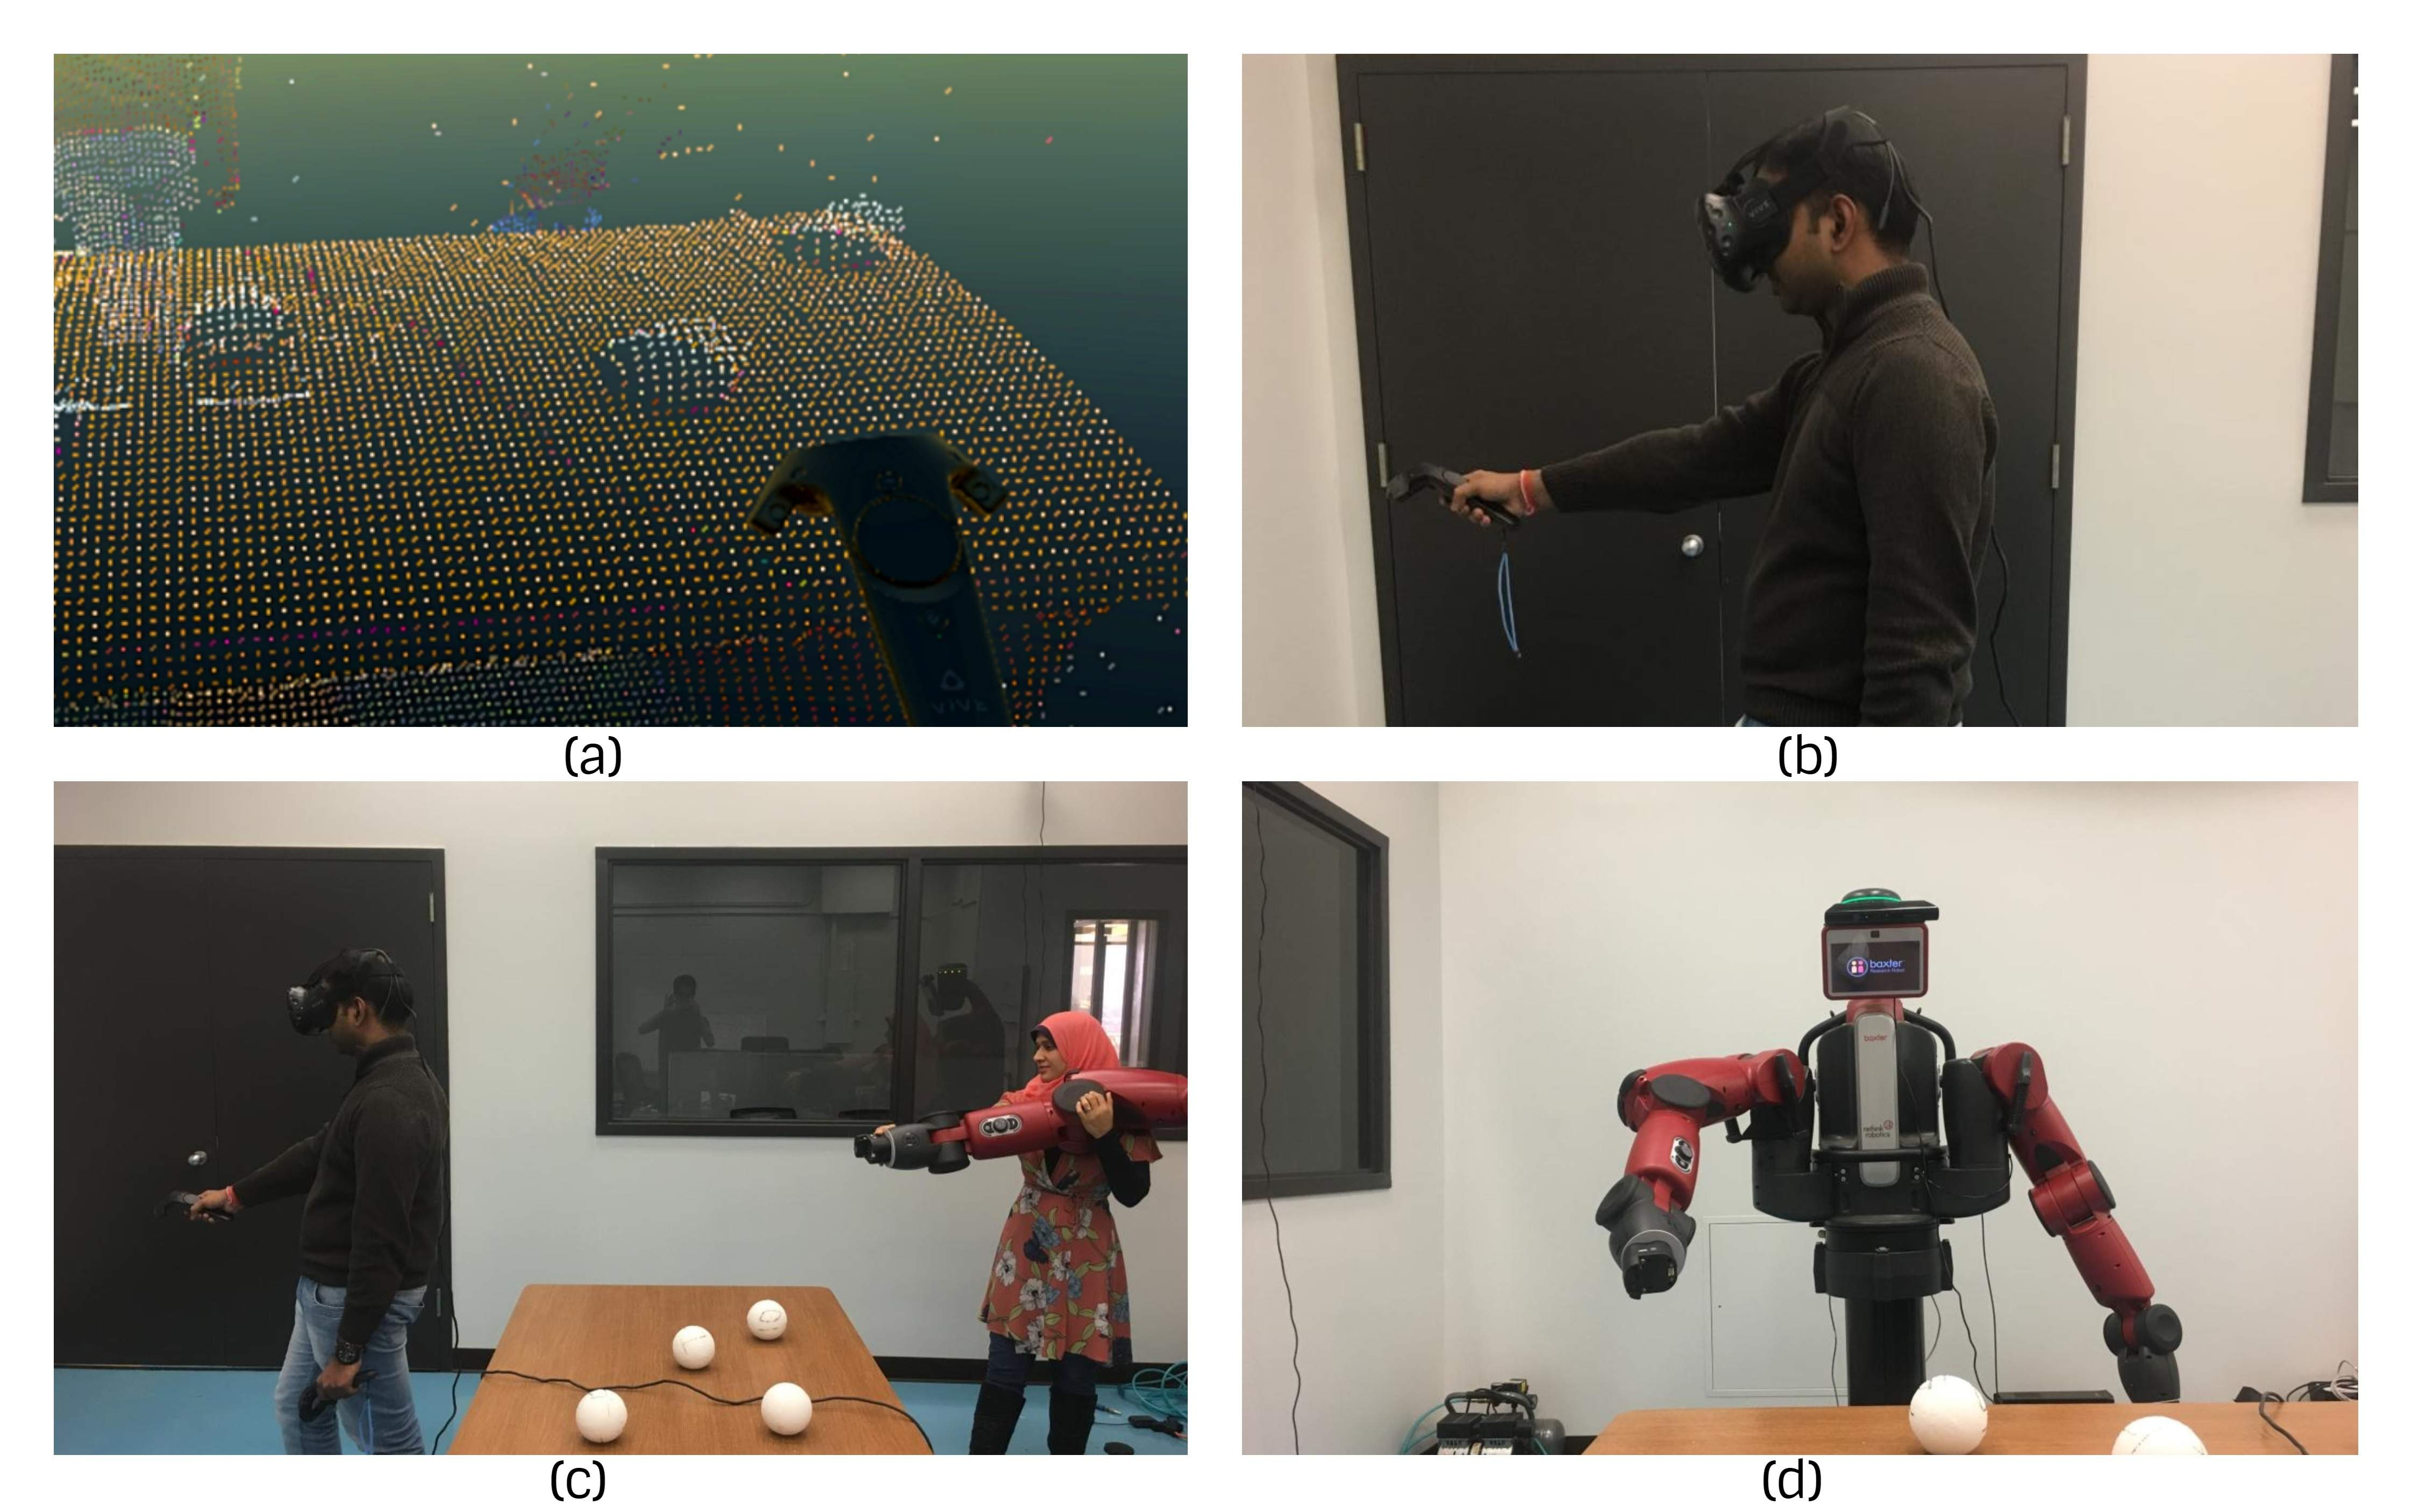
\includegraphics[width=1.0\linewidth]{fig//vive-baxter.jpg}
%   }
% \caption{(a) Visualization of Baxter workspace from Microsoft Kinect Camera to HTC Vive; (b) Operator holding HTC Vive controller slowly moves his hand from neutral position; (c) trainer moves robot hand manually to follow human trajectory; and (d) Baxter reaching the same configuration as human operator.}
% \label{fig:vive}
% \end{wrapfigure}
\noindent

%-------------------------------------------------------------------------
\subsubsection{Activity 3.1 --- Implementation}\label{sec:plan-evaluation-implementation}
%-------------------------------------------------------------------------
This activity aims to implement methods proposed in Activity 1 and 2 on the Tele-robotic Intelligent Nursing Assistant (TRINA) system and evaluates their efficacy over the nursing tasks in~\fig{Tasks}. Here we describe the demonstration tasks in details with the lifelong learning and intent inference methods evaluated through them. 

\paragraph*{Moving a patient transfer bed} This task requires the teleoperated nursing robot to collaboratively move a patient transfer bed with an on-site nurse from the entrance of a simulated patient room to the side of a patient bed. This task aims to evaluate the robot's capability of learning and updating abstract task structure, motion primitives and shared object affordance (Activity 1). From the expert demonstrations, the robot develops its capabilities of: (1) shared intent forecasting of high-level tasks, sub-tasks, and role assignments (Activity 2.1), (2) intent forecasting of subtasks from motion primitives through robot mediated demonstrations (Activity 2.1). We will also show if the robot can infer the strategy for motion coordination and use shared-autonomous control module to assist novice teleoperator in the coordination of manipulation and navigation (Activity 2.3). 

\paragraph*{Organizing and cleaning} In this task, the teleoperated nursing robot will collaborate with a on-site human nurse to organize the medical supplies scattered on a work station to their containers. They will also work together to clean the patient room debris, including dirty beddings and clothings from the patient bed, and the suction and urine containers. In this collaboration, the human nurse is responsible for the task steps that require high motion dexterity (e.g., unplugging the suction container from the suction system) and involve intimate physical human robot interactions (e.g., taking off the dirty clothing from the patient body). The robot is responsible for collecting or disposing the debris, and handle the object received from its human partner. This task aims to evaluate the robot's capability of learning and updating collaborative task structure and low-level motion skills (Activity 1). It aims to enable the robot to learn the preferred task-sharing resulted from the explicit and implicit negotiation between the end user and expert teleoperator, and how to maximally utilize its physical capability (Activity 2.1 and 2.2). Through this task, we will also demonstrate how to use active intent detection to assist a novice user in dexterous manipulation (Activity 2.4).  

\paragraph*{Preparing and Serving food} In this task, the nursing robot will load food tray with containers for food, beverage and medicine cups, bring the prepared tray close to patient bed, and serve them to the patient lying in bed. This task aims to evaluate robot's capability of learning and updating abstract task structure, motion primitives, as well as individual and shared object affordance (Activity 1). It also develops the robot's capability of fast action recognition and real-time motion prediction during human-robot handovers (Activity 2.2). 



% %-------------------------------------------------------------------------
% \subsubsection{Activity 3.2 --- Evaluation metrics for user study and }\label{sec:plan-evaluation-evaluation}
% %-------------------------------------------------------------------------
% \noindent

% We will also introduce our experiments for collecting demonstrations from human teachers and validating with novice teleoperators, as well as our proposed evaluation metrics. 

% We plan to collect demonstrations from the robot-mediated interactions/collaborations between expert teleoperator and end users. The nursing tasks we consider include: 




% Although the human nurse and nursing robot do not manipulate shared object, yet their choice of the objects to manipulate affect each other's task-sharing. Thus, The assistive module will first suggest to the novice teleoperator which objects the robot can handle given its physical capbilities.

% Here we consider the nursing task of collaboratively clearning patient room, which involves: removing the dirty beddings and clothings from the patient bed, and removing patient rooms debris such as suction and urine containers. In this collaboration, the human nurse is responsible for intimate physical human robot interactions (e.g., taking off the dirty clothing from the patient body), and manipulations that requires fine motor skills (e.g., removing suction container from the suction system). The robot is responsible for collecting or disposing objects the nurse hand over or leave to it. Under this task scope, we illustrate the function of the assistive module in two typical scenarios: \textit{Cooperative Mode} --- The robot takes and places the object handed over by the human nurse; and \textit{Collaborative Mode} --- The robot and nurse need to pick and place a collection of objects. 

% \paragraph*{Cooperative mode} In the first scenario, the human nurse and nursing cooperatively manipulate a shared object. When taking an object from the human nurse, the assistive module will utilize the knowledge of shared object affordance and automatically identify where the robot should grasp given where the human nurse has grasped. The robot will also use the learned interactive motion primitives to predict human partner's motion and plan its responding motion. 

% \paragraph*{Collaborative mode} In this scenario, 

% \paragraph*{Prepare and Serve food}

% (1) Task description

% (2) Method required 

% - Learning abstract task structure

% - Learning motion primitives

% - Human-robot handing over - action recognition + real-time motion prediction 

% \paragraph*{Moving patient bed}
 
% (1) Task description  

% (2) Method required  

% - Learning abstract task structure

% - Learning motion primitives

% - Learning collaboration goal using bayesian framework

% Grasping - Given where the human nurse grasp on the bed, where the robot should grasp on the shared object

% Collaborative Moving - Follow the moving direction guided by the human nurse

% Learn joint action affordance; Learn robot task-goal constrained by shared object goal state and human partner's action

% - Learning expert teleoperator intent --- an reward function for whole-body motion coordination, to assist novice teleoperator to  move mobile automatically to facilitate manipulation 


% \paragraph*{Organizing and cleaning patient room}

% - Learning abstract task structure

% - Learning motion primitives

% - Learning collaborative task decomposition (Stackburg)

% Collaborative object organization - Learn to match user preference to object affordance features



% Compensate for inaccurate motion of novice user - interactive intent detection

% Although it is possible to map the teleoperator's whole-body motion to using a motion capture system or exoskeleton, 

% user interface,     

% Our mobile base motion control strategy is concerned of (1) facilitating the manipulation tasks being performed, and (2) behaving appropriately in human environment and to human partners. Here we apply the low-level coordinated motor skills and high-level task knowledge developed in Task 1, to assist novice teleoperator in the task of nursing tasks such as collaborative moving a patient transfer bed. 

% % Investigate the high-level strategies for coordination of mobile manipulator systems that consists of hierarchical macro- and micro-structures.

% social focal point (equilibrium - navigation in human environment)


% \paragraph*{Problem Formulation} 

% 	* When and how to move the mobile base (in relation to hybrid system theory, region of attractions in each stable mode (mobile base navigation control and manipulator control)).
% 	* Coordination of macro- and micro-structure
% 	* Related work on mobile manipulator, and micro-/macro-structure coordination



% Given that human nurse is superior in perception and motion capability, it is very possible that the human nurse will finish their preferred and manageable task 


% As the collaboration goes on, fewer objects will be left for pick and place. These objects are left for human nurse is unwilling to handle it, or needs the nursing robot's help for operation. In this case, the robot will add the remaining object to when its priority-based task queue is empty. The robot will first attempts  

% In this collaborative task, the human nurse is responsible for intimate physical human robot interactions (e.g., taking off the dirty clothing from the patient body), and manipulations that requires fine motor skills (e.g., removing suction container from the suction system). The robot is responsible for collecting or disposing objects the nurse leaves behind or hand over to it. 

% 

% \paragraph*{Collaborative mode} In the first scenario, 

 

% \paragraph*{Cooperative mode} In the second scenario, the human nurse and nursing cooperatively manipulate a shared object. Thus, the assistive module will shared object affordance, automatically identify where the robot should grasp given where the human nurse has grasped on the object being handed over. 



% In case of ambiguity, the teleoperation system takes the implicit judgment from the teleoperator expressed in teleoperator's subtle reaction.   


% a hierachical data structure which prioritizes the operatable objects by their distance to the robot hands, and prioritizes an object affordance feature by the easiness of the operation. 



%  for 

% probabilistic model 

% of where what and where the teleoperator may potentially operate on. 


% From the robot-mediated collaboration demonstrated by the on-site human nurse and expert teleoperator, the robot has learned the (shared) object affordance. 















% based on interactive motion intent inference. Exploit knowledge of task affordance and multi-agent interaction modeling to improve the fluency coordinated and collaborative manipulation.



% \paragraph*{Vocabulary and Semantics for complex motion intent}

% \paragraph*{Non-intrusive manipulation assistance based on interactive intent inference and task affordance learning} 

 
% We propose a scenario that a novice teleoperator control a tele-nursing robot with an end user whose at least more capable in motion than the teleoperated robot; In this case, the human end user (either a human nurse or a patient that is still capable to move) will take the lead in human-robot interaction.  

% The teleoperator's operation is closely associated to the task/object affordance, and in response to the end user's motion. 

% As a result, the teleoperation system will infer the human teleoperator's motion intent, based on the learned object/task affordance, as well as the end user's motions




%-------------------------------------------------------------------------
\subsubsection{Activity 3.2 --- Evaluation metrics for user study}\label{sec:plan-implementation-userstudy}
%-------------------------------------------------------------------------
The proposed research involves human subjects in both robot learning and system evaluation. Given the nursing tasks shown in~\fig{Tasks}, we will first teach experienced nurses to control the nursing robot in direct teleoperation, and then collect their robot-mediated collaborations with their human partners in a simulated patient room. To record the nurses' learning curve, we will repeat the cycle of teleoperation training and task performing, until the nurse under training can successfully teleoperate the robot to finish the collaborative task. For system evaluation, we will teach experienced nurses new to the nursing robot to learn to control the robot with the developed assistive modules, and perform the same set of collaborative nursing tasks. We compare the learning curve of the teleoperator nurses with and without the assistive modules, to validate effects of robot learning.

This activity aims to develop systematic metrics for evaluating the capability of lifelong learning and intent inferences, and for comparing the user experience under shared-autonomous control and direct teleoperation. Through the nurse's learning process, we observe the change in task completion time, success rate, error type and frequency. We use NASA Task Load Index (NASA-TLX) to evaluate the experience of expert and novice teleoperator and end users, to measure their physical, mental, temporal demands as well as effort and frustration in robot teaching and using. Through questionnaires, we will investigate: (1) Does the autonomous motion coordination comply with the manipulation they intend to perform? (2) Does the robot adapt quickly to their preference of task operation? (3) Does the robot behaves naturally to the on-site human partner? (4) Do the assistive modules facilitate them learning the motion correspondence between the robot and operator, and therefore reduce operator training effort? Through the user study, we aim to answer a general research question of what level of motion intelligence should a mediating robot develop to support the level of shared-autonomy. 



% The subjects will also report their preference for the assistance provided by different levels of autonomous control. Under shared autonomy, do human operators/end users prefer more or less dominance in control? Are their preferences task-dependent (e.g., depending on whether the operation involves intimate human-robot interactions), skill-dependent (e.g., depending on their experience with computers, video games or nursing experience), or scenario-dependent (e.g., whether the operator needs to be engaged with the end user in communication, attention and emotion)? In a previous user study, the PI has observed preferences for both more and less dominance of the operator in shared autonomous control. On one hand, more direct control over the robot may be preferred because the operator and/or end user have a plan in mind for the manipulation particularly for sequential tasks. The robots are neither able to work out a better plan nor able to infer their intention well. On the other hand, more supervisory control is favored in the scenarios where engaged communication was as important as the operation being performed, such as in patient care. 

% Many collaborative nursing tasks, such as removing a heavy blanket from patient

% The developed motion intelligence can be applied to autonomous navigation strategy that facilitates the manipulation tasks under direct teleoperation, and provide adaptive assistance to novice user in dexterous manipulation tasks. 



% More evaluating the capability of the developed motion intelligence, our implementation and user study on TRINA system aims to provide a paradigm that can improve the adaptability via the practice of robot-mediated collaboration.

% %-------------------------------------------------------------------------
% \subsubsection{Benchmark}\label{sec:plan-implementation-userstudy}
% %-------------------------------------------------------------------------





%-------------------------------------------------------------------------
\section{Broader Impacts}\label{sec:impact}
%-------------------------------------------------------------------------

% Broader impacts may be accomplished through the research itself, through the activities that are directly related to specific research projects, or through activities that are supported by, but are complementary to, the project. NSF values the advancement of scientific knowledge and activities that contribute to achievement of societally relevant outcomes. Such outcomes include, but are not limited to: full participation of women, persons with disabilities, and underrepresented minorities in science, technology, engineering, and mathematics (STEM); improved STEM education and educator development at any level; increased public scientific literacy and public engagement with science and technology; improved well-being of individuals in society; development of a diverse, globally competitive STEM workforce; increased partnerships between academia, industry, and others; improved national security; increased economic competitiveness of the United States; and enhanced infrastructure for research and education.

\paragraph*{Broader Technological and Societal Impacts} 

This project envisions broader impacts on  ... 
% This project envisions broader impacts on rehabilitation, assistance exoskeletons and prosthetic upper limbs that are expected to render human-like motions. For instance, our proposed motion control method can enable robotic exoskeletons to be more transparent to healthy operators, and to correct abnormal joint coordinations resulting from motor disabilities. The proposed project will also benefit a wide range of arm-like robotic manipulator robots for medical, industrial and military-relevant tasks, such as redundant manipulators for minimally-invasive surgery, humanoids for manufacturing and maintenance, and mobile manipulators for explosive ordnance disposal. Our research effort aims to remove two major barriers that prevent robot merging into human society as capable and socially acceptable peers: robots should be able to \textit{move like humans} and \textit{work with human-level motor skills}. Results from investigating human-inspired robotic motion control also help validate our understanding of human motion control, and therefore have broader impact on the training and recovery of human motor skills. By improving the usability of dexterous robotic manipulators under direct teleoperation and shared-autonomous control, this project may also lead to improved availability of healthcare and industrial labor, and provide surrogates for military and medical personnel for tedious, repetitive, and dangerous tasks. It also aims to enable the creation of more human-like and human-friendly robots for hospital and home care that can provide long-term assistance to aging and disabled populations.


\paragraph*{Integrating Research with Education} 

The proposed research will be integrated with undergraduate and graduate course offered by the WPI robotics engineering program (RBE). The humanoid nursing robot will serve as infrastructure for both research and education. In Fall 2017, the PI will begin teaching an innovative course (Synergy of Human and Robotic Systems) on the design and motion control of human-compatible and human-like robots. This course is currently offered as a robotics engineering course, and will be extended as cross-curricular course for both robotics engineering and mechanical engineering. Students will actively participate in the research via their course projects. Toward the goals of the proposed research, the PI is also advising three Major Qualifying Project (MQP) teams working on humanoid manufacturing/nursing robots in the 2017-2018 academic year. These MQP projects include: (1) arm-hand and bimanual coordination of a humanoid robot for shoe-sewing tasks, (2) human-inspired design and motion control of multi-fingered grippers for dexterous manipulation, and (3) developing an intuitive motion control interface to reduce the training effort of novice teleoperators. The MQP project on the humanoid manufacturing robot has received industrial funding and hardware support from New Balance. Further support for graduate-level research will be considered based on the outcome of the MQP.

% This project aims to achieve broader technology impacts and contribute to innovative education, outreach and diversity activities: 


% It can also be applied to maintenance which need to perform precise and dexterous manipulation, and service and assistive robots which are expected to . 


% By investigating human-inspired robotic motion control, it promotes the synergy of robots and human. 

\paragraph*{Diversity and Outreach Activities}
Beside education activities at WPI, this research will engage research and teaching faculty and students from the nursing school of Worcester State University, and promote education around tele-robotic approaches for healthcare. It aims to encourage woman students in the nursing school to actively participate in the development of the humanoid nursing robot by providing valuable insights and experience from their nursing education and practice. It will also prepare students of the nursing school for a new generation of medical robotic technologies that will be widely available in near future. To promote K-12 education, the humanoid nursing robot will be offered as an educational platform through WPI First Robotics Competition, and will be open to the general public at the WPI TouchTomorrow robotic event. The PI's lab will reach out to local underprivileged high schools and organize free robotics workshops and open lab events for their students. This research will also contribute to the Robotics Education program between WPI and the Worldbank for Sub-Saharan Africa, to promote STEM practice and engagement amongst high school students using robotics. 

\paragraph*{Broader Dissemination}
This research will produce academic journal and conference publications, as well as mathematical human motion models, human motion data and software packages released on the World Wide Web. Software packages that implement the proposed motion control methods will be developed for compatibility with Robot
Operating System (ROS), OpenRave and Open Motion Planning Library (OMPL). Based on the research, the PI plans to organize a workshop at an international robotics conference (IROS or EMBC) on human-inspired design and motion control. Course Materials (lecture notes, homework, project design, etc.) based on the proposed research will also be shared on the PI's research website. Overall, this research will improve the well-being of individuals in society, contribute to the development of a diverse, globally competitive STEM workforce, and increase economic competitiveness of the United States.

% In 2017 Fall, the PI will teach a graduate course of synergy of human and robotic systems at WPI. This course covers the design and motion control of human-compatible and human-like robots, and will include the proposed Task 1 and 2 as course projects. Two Major Qualifying Project (MQP) teams the PI advises in 2017-2018 academic year will work on vision-based shared-autonomous control of a humanoid manufacturing robot, and the design and motion control of a dexterous robotic hand for precise manipulation. This research will actively engage K-12 students through WPI robotic events open to the general public, such as TouchTomorrow and FirstRobotics Competition. 

%-------------------------------------------------------------------------
\section{Results from Previous NSF Support}\label{sec:priorNSF}
%-------------------------------------------------------------------------

PI Zhi Li has not received prior NSF support.

\textbf{B. Ziebart} was a sub-contractee on NRI-\#1227495 (\$509,409,
10/2012-9/2017),``Collaborative Research:
Purposeful Prediction: Co-robot Interaction via Understanding Intent
and Goals,'' is a PI on RI-\#1526379 (\$500,000, 09/2015-8/2018),
``Robust Optimization of Loss Functions with Application to
Active Learning'') and is a PI on III-\#1514126 (\$636,454, 09/2015-08/2018)
``Collaborative Research: Computational tools for extracting individual,
dyadic, and network behavior from remotely sensed data.''
The {\bf Intellectual Merits} for these awards include: the
creation of a framework enabling robots to anticipate and adapt to the
activities of their human co-workers (NRI); developing techniques that
better align learning objectives with application performance measures
in classification settings (RI);
and developing methods for making sense of massive amounts of social animal
sensor data (III).
The {\bf Broader Impacts}
include the significant efficiency improvements in small- and
medium-scale manufacturing that these improved interaction technologies
will facilitate (NRI); improving the application of machine learning to a
range of domains with non-convex loss measures
(RI); and effectively multiplying the expertise
of field biologists when interpreting sensor data (III).
To date, these projects have produced
a total of ten conference publications and six workshop publications
covering the topics of
inverse optimal control \cite{asif2013inferring,monfort2013predictive,
byravan2014layered,monfort2015intent,chen2015predictive,
byravan2015graph,monfort2015softstar,chen2015imitation,chen2016adversarial},
learning under covariate shift/active learning
\cite{liu2014robust,liu2015shift,liu2015addressing,chen2016robust},
inductively optimizing multivariate losses \cite{wang2015adversarial},
sequence prediction \cite{li2016adversarial}, and learning to interact
\cite{behpour2015minimax}.

\textbf{J. Fu} is the Co-PI of
\underline{CMMI-1728412}: \textbf{Intelligent Soft Robot Mobility in
  the Real World,} (PI: C. Onal, $200,000$ for Co-PI J. Fu, 08/15/2017
- 07/31/2020). \textbf{Intellectual Merit:} The proposed research will
advance soft robot intelligence and mobility in uncertain real-world
environments that cannot be safety traversed using rigid robotic
systems.  \textbf{Broader Impact:} This research will pave the way for
soft robots to be utilized at farms, homes, manufacturing sites, and
search and rescue scenarios. It will have impacts on education in
robotics.

% %-------------------------------------------------------------------------
% \section*{APPENDIX}
% %-------------------------------------------------------------------------

% Appendixes should appear before the acknowledgment.

% %-------------------------------------------------------------------------
% \section*{ACKNOWLEDGMENT}
% %-------------------------------------------------------------------------
\pagebreak
\setcounter{page}{1}
\setcounter{section}{0}
\pagebreak

\begin{center}
	{\Large \bf Supplementary Documents --- Collaboration Plan}\\
%     \vspace{4pt}
% 	\renewcommand{\baselinestretch}{1}
%    	{\large PI: Zhi Li (Worcester Polytechnic Institute)\\
%     Co-PI: Brian Ziebart (University of Illinois at Chicago), Jie Fu (Worcester Polytechnic Institute)}
   	% \vspace{4pt}
    % {\large Worcester Polytechnic Institute}
\end{center}

\vspace{0.5em}

% an old template 



\noindent
{\bf Personnel:} 
This project will be carried out by the PIs and three Ph.D. students at WPI and UIC. 

\bigskip 

\noindent
{\bf Coordination:}
The project teams will meet weekly via video conference (e.g., Skype) and meet in person semi-annually to coordinate research efforts. They will set up a project management system using Slack (or similar) to facilitate offline communication and collaboration among the team members.

\bigskip

\noindent
{\bf Shared Code Repositories and Common Robot Infrastructure:}
A simulation of the TRINA system is currently available so that algorithm development and implementation can be conducted in parallel at WPI and UIC. The team members will share software developed through ROS packages and the TRINA software stack. The system evaluation will primarily be conducted at WPI with the full TRINA system, while the UIC laboratory will work on a partial demonstration using its Baxter robot from ReThink Robotics. Evaluation of intent prediction algorithms can be performed both with TRINA systems or other human-robot or human-human collaborative tasks.  The experimental validation will involve undergraduate students through summer internships or senior design projects. 

\bigskip

\noindent
{\bf Schedule of Research Efforts:}
The anticipated schedule for the major tasks is shown in~\fig{fig:timeline} (Blue marks are milestones for Task 1 and 2, respectively).

%\vspace{-2ex}
%\begin{wrapfigure}{r}{0.45\textwidth}
\begin{figure}[h]
\begin{center}
\noindent\resizebox{0.7\textwidth}{!}{
\begin{tikzpicture}[x=.5cm, y=0cm]
\begin{ganttchart}[y unit title=0.5cm,
y unit chart=0.5cm, vgrid, title/.style={fill=black!60, draw=none},
title label font=\color{white}\bfseries \small,
hgrid, % title label font = \small, title height=.8,
bar label font=\small, 
bar label node/.append style=%
{align=left},
milestone height = 0.15mm,
milestone/.append style={fill=blue!80}, 
%  milestone label node/.append style={anchor=south}, 
milestone label font = \small\bfseries,
group label font =\small\bfseries\color{blue}, bar height=.4, bar
group/.append style={draw=black, fill=blue!20},]{1}{12}
\gantttitle{Year-1}{4} \gantttitle{Year-2}{4}\gantttitle{Year-3}{4} \\
\ganttgroup[name=task1]{Task 1}{1}{6}\\
\ganttbar[name=data]{Data collection and segmentation (1.0)}{1}{8}\\
\ganttbar[name=dmpLearn]{Learning coordinated and interactive motion primitives (1.1)}{1}{4}\\
\ganttbar[name=taskLearn]{Learning task constraints and dependency (1.2)}{3}{6}\\
\ganttbar[name=adaptation]{Personalized adaptation of motor skills (1.3)}{4}{6}
\ganttmilestone{}{6} \\
\ganttgroup{Task 2}{1}{8}\\
\ganttbar[name=irlGame]{Inference of shared intent (2.1)}{1}{3}\\
\ganttbar[name=intentDetect]{Task step recognition from partial motion (2.2)}{3}{4}\\
\ganttbar[name=coordination]{Autonomous coordination of navigation and manipulation (2.3)}{5}{6}\\
\ganttbar[name=motionPredict]{Active intent detection in user assistance modules (2.4)}{6}{8}
% \ganttmilestone{Milestone: Task 2}{8} \\
\ganttmilestone{}{8} \\
\ganttgroup{Task 3}{4}{12}\\
\ganttbar[name=experiment]{Evaluation of intent and motion prediction (3.1)}{4}{12}\\
\ganttbar[name=nav]{Developing assistive modules in TRINA (3.2)}{6}{8}\\
\ganttbar[name=manipulation]{System integration and evaluation (3.2)}{6}{10}\\
\ganttbar[name=userStudy]{User study (3.1,3.2)}{4}{12}
% \ganttlink{intentDetect}{nav}
% \ganttlink{taskLearn}{nav}
% \ganttlink{dmpLearn}{manipulation}\
% \ganttlink{irlGame}{manipulation}
% \ganttlink{intentDetect}{manipulation}
 \end{ganttchart}
 \end{tikzpicture}
 }
 \end{center} %\vspace{-4ex}
\caption{\small Project Timeline. \label{fig:timeline}}
\end{figure} 
\vspace{2ex}

\noindent
PI Li will lead the research efforts for Tasks (1.0),(1.1) (1.3) (2.3) and (2.4). PI Ziebart will lead the research efforts for Tasks (2.2); PI  Fu will lead the research efforts for Tasks (1.2) and (2.1). Li and Fu will collaborate to construct consistent high-level task decompositions and low-level dynamic movement primitives from human demonstrations. Fu and Ziebart will collaborate on shared intent inference with the game-theoretic formulation and develop theory and algorithms for online active intent detection. Li and Ziebart will collaborate on Task (2.3) and (2.4). Li will lead the research efforts for Task 3, and collaborate with Ziebart and Fu on implementation and user study.
\pagebreak
\setcounter{section}{0}
\pagebreak

\begin{center}
	{\Large \bf Supplementary Documents --- Human Subjects Protection}\\
%     \vspace{4pt}
% 	\renewcommand{\baselinestretch}{1}
%    	{\large PI: Zhi Li (Worcester Polytechnic Institute)\\
%     Co-PI: Brian Ziebart (University of Illinois at Chicago), Jie Fu (Worcester Polytechnic Institute)}
   	% \vspace{4pt}
    % {\large Worcester Polytechnic Institute}
\end{center}

\vspace{0.5em}

Both the University of Illinois at Chicago and Worcester Polytechnic Institute will have their Institutional Review Board (IRB) review all research involving the use of human subjects. All PIs are familiar with IRB policies, including fulfilling the required continuing training in human subjects protection.

We will submit an IRB protocol to cover the collection of human demonstration and the user study for system evaluation. We foresee that the IRB will review the protocol under expedited procedure, since it is minimal risk. Our study aims to demonstrate the system usability and will be performed in simulated patient room. We will have healthy subjects to play the roles of patients. No real patients will be involved.

%-------------------------------------------------------------------------
\section{Data collection}\label{sec:data}
%-------------------------------------------------------------------------

Our experiment will record robot and human motions in robot-mediated nursing tasks, using cameras, a motion capture system, and robot sensors. We will record full body motion and audio of the participants and collect questionnaires to evaluate user experience. All the data will be de-identified for privacy and confidentiality. 

%-------------------------------------------------------------------------
\section{Potential Risks}\label{sec:risk}
%-------------------------------------------------------------------------
The risks in robot teleoperation and interaction are minimized. The humanoid robot involved in this experiment is the Baxter robot from Rethink Robotics. This robot is designed to work safely and efficiently alongside people. In particular, it has safety and compliance features that slow or stop upon inadvertent contact, which allows it to work collaboratively or to be co-located with an operator in close proximity. The Baxter robot has a wide array of innovative sensors, and an emergency stop (E-stop) function to ensure safety, which will be carefully administrated by a trained experimenter. In the event of a power loss or an E-stop, the robot slowly comes to rest. Baxter’s arms, which will physically interact with the subjects, weigh less than 20 kg, are fully covered in compliant plastic, and use protective foam at key joints. Baxter can recognize human proximity with its $360^\circ$ sonar system, which signals its awareness of any detected nearby people. The Baxter robot meets the applicable parts of ISO 10218-1. 

Given the intrinsically safe robot platform, the potential risk of this study may include: (1) physical and mental fatigue in robot teleoperation and interaction, (2) the confidentiality of collected data that may reveal the participant identities. 

%-------------------------------------------------------------------------
\section{Recruitment and informed consent}\label{sec:consent}
%-------------------------------------------------------------------------
% PM: IIRC normal age of consent is 18? Why choose 21?
We plan to recruit 20-30 adults over age 18 who are capable of providing consent. The on-site research assistant will be available to discuss the risks and benefits of the study and answer any questions. The following will be explained: (1) purpose; (2) financial compensation for completing the study; (3) types of data collected; (4) virtual and human coach interventions; (5) measures to ensure confidentiality of data collected; and (6) timeline. Regarding data collection, subjects will be made aware of the methodology, including all the data being recorded. They will also be informed that, if they provide separate consent, their de-identified data will be released to other research groups at the end of the project.
% PM: I'm not sure why you're sending text messages to participants, and nothing you've mentioned so far suggests this? Maybe just get rid of this sentence?


%\subsection*{Inclusion of women, minorities and children}
\paragraph{Inclusion of women, minorities and children.}
We plan to recruit only adults over age 18 who are capable of providing consent. For the present study, neither minors nor persons with without motor, vision, hearing, cognitive impairments will be recruited. We will recruit women and minorities to ensure that our human subjects are representative of the general population and of nursing professionals. 

%\subsection*{Planned procedures to protect against or minimize potential risks}

%-------------------------------------------------------------------------
\section{Planned procedures to protect against or minimize potential risks}\label{sec:protection}
%-------------------------------------------------------------------------
To protect against the minimal risks involved in robot teleoperation and interaction, the experiment trials will be broken into several exercises expected to take no more than 20 minutes each, and subjects may take breaks between exercises. The experiment will only continue if the subject feels comfortable to continue. The subject can ask to terminate the experiment at any time he/she wants. If any emergency happens, the experiment administrator will call 911.

As concerns privacy and confidentiality, we will keep de-identified data on password-locked computers, including one of the servers in PI Ziebart's laboratory in the Science and Engineering Laboratories building of UIC, and one of the servers in PI Li's laboratory in the Robotics Engineering Program at WPI. Both laboratories are locked and only the PIs and their graduate assistants have access. The data will be accessible only to the PIs and their graduate assistants. The data will be stored on different servers because software tools that are needed to process the data are not available on every server, e.g. because of licensing issues.
\pagebreak
\setcounter{section}{0}
\pagebreak

\begin{center}
	{\Large \bf Supplementary Documents --- Data Management}\\
%     \vspace{4pt}
% 	\renewcommand{\baselinestretch}{1}
%    	{\large PI: Zhi Li (Worcester Polytechnic Institute)\\
%     Co-PI: Brian Ziebart (University of Illinois at Chicago), Jie Fu (Worcester Polytechnic Institute)}
   	% \vspace{4pt}
    % {\large Worcester Polytechnic Institute}
\end{center}

\vspace{0.5em}
%-------------------------------------------------------------------------
\section{Roles and responsibilities}\label{sec:resp}
%-------------------------------------------------------------------------

PI Li, Fu and Ziebart (referred as “the PI” in this document) will be jointly responsible for data management and for monitoring the data management plan. They and their PhD students working on the proposed project under their supervision will adherence to this data management plan be checked or demonstrated. They have responsibility over time for decisions about the data once the PhD students are no longer available.

%-------------------------------------------------------------------------
\section{Types of Data and Policies for Storage}\label{sec:type}
%-------------------------------------------------------------------------
The data and materials expected to be produced will include computational codes, software, raw data files from experiments, data analysis files, simulation data, video recordings of experiments, etc. Each class of data is described below:
\begin{itemize}	

\item Experimental data: The data collected in the experimental user study include: 
\begin{itemize}
\item Kinematic motion data, i.e., the 3-dimensional position of the passive reflective markers attached to the human subjects recorded using a Vicon motion capture system and saved in .csv and .c3d formats.
\item Digital video and audio data that record the experiment trials.
\item Subjects’ biometric information for data analysis, such as age, gender, height, and weight.
\item Subjects’ personal information for contact, including name, phone number, and email.
\end{itemize}

Data from each subject will be stored in password-protected computers under the subject ID automatically generated by the motion capture system. Access to the data is limited to faculty and students working on the proposed project and requires the PI’s permission. The retained copy of the videotape of subjects’ motion will be processed so that the faces of the subjects are blurred to be unrecognizable, and will only be disseminated with the consent of the subject in the video. Hard copies of the questionnaires and consent forms will be shredded and discarded. The motion data, video, audio, and subject’s biometric information will be used for research purposes and retained indefinitely. Personal information will be kept confidential and will be discarded as soon as the experiments are completed. No identifiable information will be recorded or used for the purpose of study.

\item Computational codes and software development data

This data includes Matlab, OpenSim, Robot Operating System (ROS), and customized robot control software codes (in C/C++/Python languages) for simulations and experiments. During the development, the data will be kept in a private repository managed by IT Service of Worcester Polytechnic Institute. The developed software will be maintained and accessible to the public for non-profit research after post-processing and verification of its correctness. The data will be in standard, non-proprietary file formats to facilitate both data sharing and long-term preservation.

\item Documentation for research and education activities

The research results of the proposed project will be disseminated via academic reports, software documentation and instruction manuals, lecture notes and slides, presentations, and publications. The data are saved in \LaTeX files, image files, Word/Excel/Power Point documents, and PDF files. 
\end{itemize}

\noindent
Data and metadata standards will use common ROS encodings for datasets. If any non-standard formats are used, documentation on how to use and access the data will be provided.
% PM: Changed this a bit, double-check?

%-------------------------------------------------------------------------
\section{Methods and policies for providing access and enabling sharing}\label{sec:access}
%-------------------------------------------------------------------------

The data produced in this project will not be confidential but will require the PI’s permission to access. Experimental data will be accessible only to the PI’s lab members and collaborators, while access to computational codes and software development data can be granted for non-profit academic research. Documentation for research and education activities will be available through both authors’ websites and the digital archives of the corresponding publishers. No delays in publication of the research outcomes will occur. 

%-------------------------------------------------------------------------
\section{Policies and provisions for re-use and re-distribution}\label{sec:reuse}
%-------------------------------------------------------------------------
Researchers who request the data can reuse it within the research community. The data cannot be used for commercial applications or purposes and may not be changed/resubmitted without the PI’s permission. The data is subject to WPI’s intellectual property policies.

%-------------------------------------------------------------------------
\section{Plans for archiving and preservation of access}\label{sec:axiv}
%-------------------------------------------------------------------------
The project website along with all the related material and data components will be stored on WPI servers. WPI is committed to its continuous maintenance, availability, and backups. The servers are equipped with primary and backup power, environmental, and communication systems. Physical access to this room is strictly limited to current WPI systems administrators by means of electronic locks. An alarm system that is constantly monitored by campus police has been placed to control access to the room and eliminate theft.
\pagebreak
\setcounter{section}{0}
\pagebreak

\begin{center}
	{\Large \bf Facilities and Equipments}\\
%     \vspace{4pt}
% 	\renewcommand{\baselinestretch}{1}
%    	{\large PI: Zhi Li (Worcester Polytechnic Institute)\\
%     Co-PI: Brian Ziebart (University of Illinois at Chicago), Jie Fu (Worcester Polytechnic Institute)}
   	% \vspace{4pt}
    % {\large Worcester Polytechnic Institute}
\end{center}

\vspace{0.5em}
%-------------------------------------------------------------------------
\section{Laboratories}\label{sec:Lab}
%-------------------------------------------------------------------------

PIs Li and Fu equally share a 1500 square foot lab space with another junior faculty member at WPI. This lab space is located at 85 Prescott 224, Robotics Engineering Program, Worcester Polytechnic Institute. A motion capture system has been installed in this lab to cover a 21ft by 17ft space. The rest of the lab space is sufficient for performing experimental study on humans and robots, in addition to accommodating PhD students.

PI Ziebart directs the Purposeful Prediction laboratory in the Computer Science department at the University of Illinois at Chicago (UIC). This laboratory can house 20 students and is shared with Prof. Milos Zefran, Electrical and Computer Engineering, UIC. The research focus of the lab is on the development and application of
prediction techniques for application-specific performance measures. Current application areas include robotics, human-computer interaction, and wild animal behavior and activity prediction.




% PM: Would it be useful to mention additional WPI computing resources and PI work laptops, since one desktop and one laptop seems a bit small for the number of people (2 professors + graduate students) working at WPI)?

%-------------------------------------------------------------------------
\section{Major Equipments}\label{sec:equip}
%-------------------------------------------------------------------------


\begin{figure}[h!]
\mbox{
  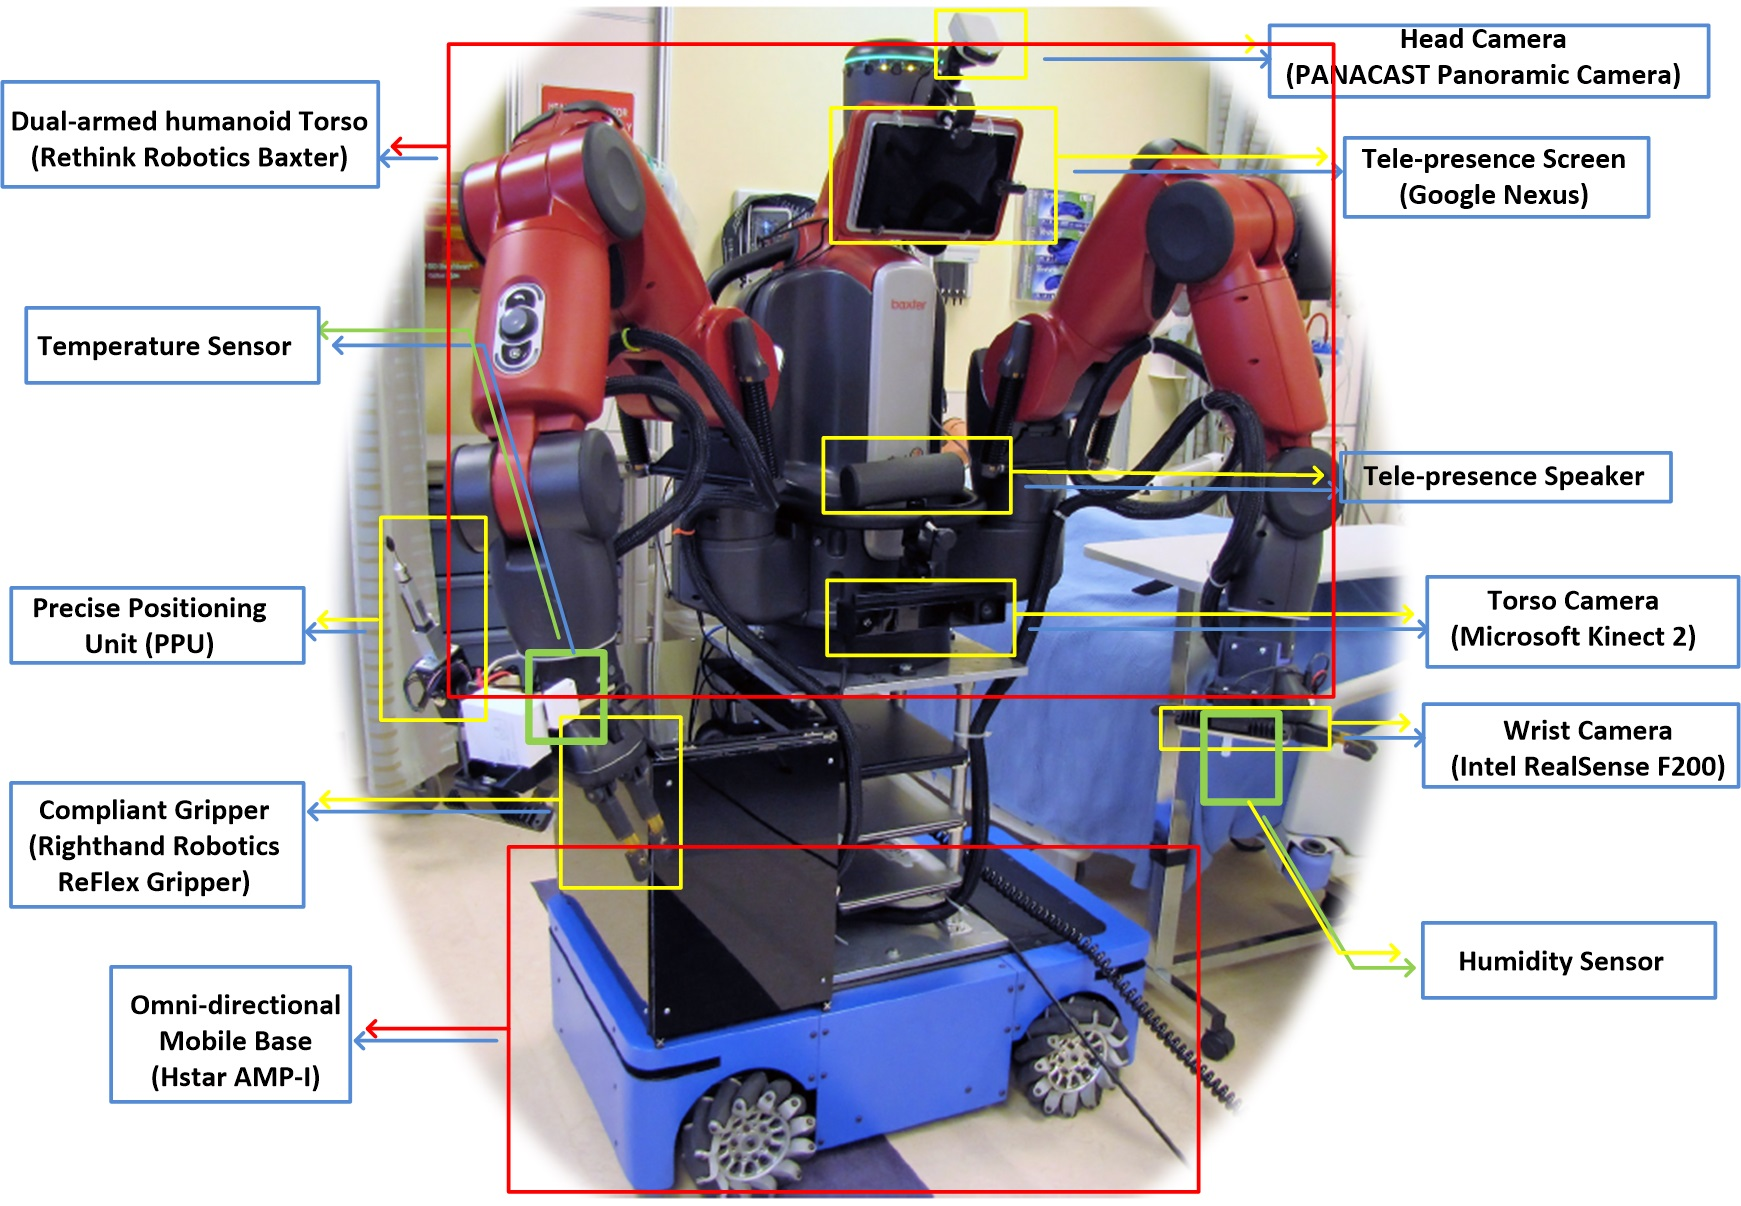
\includegraphics[width=0.48\linewidth]{fig//TRINA_Hardware_Notes}
    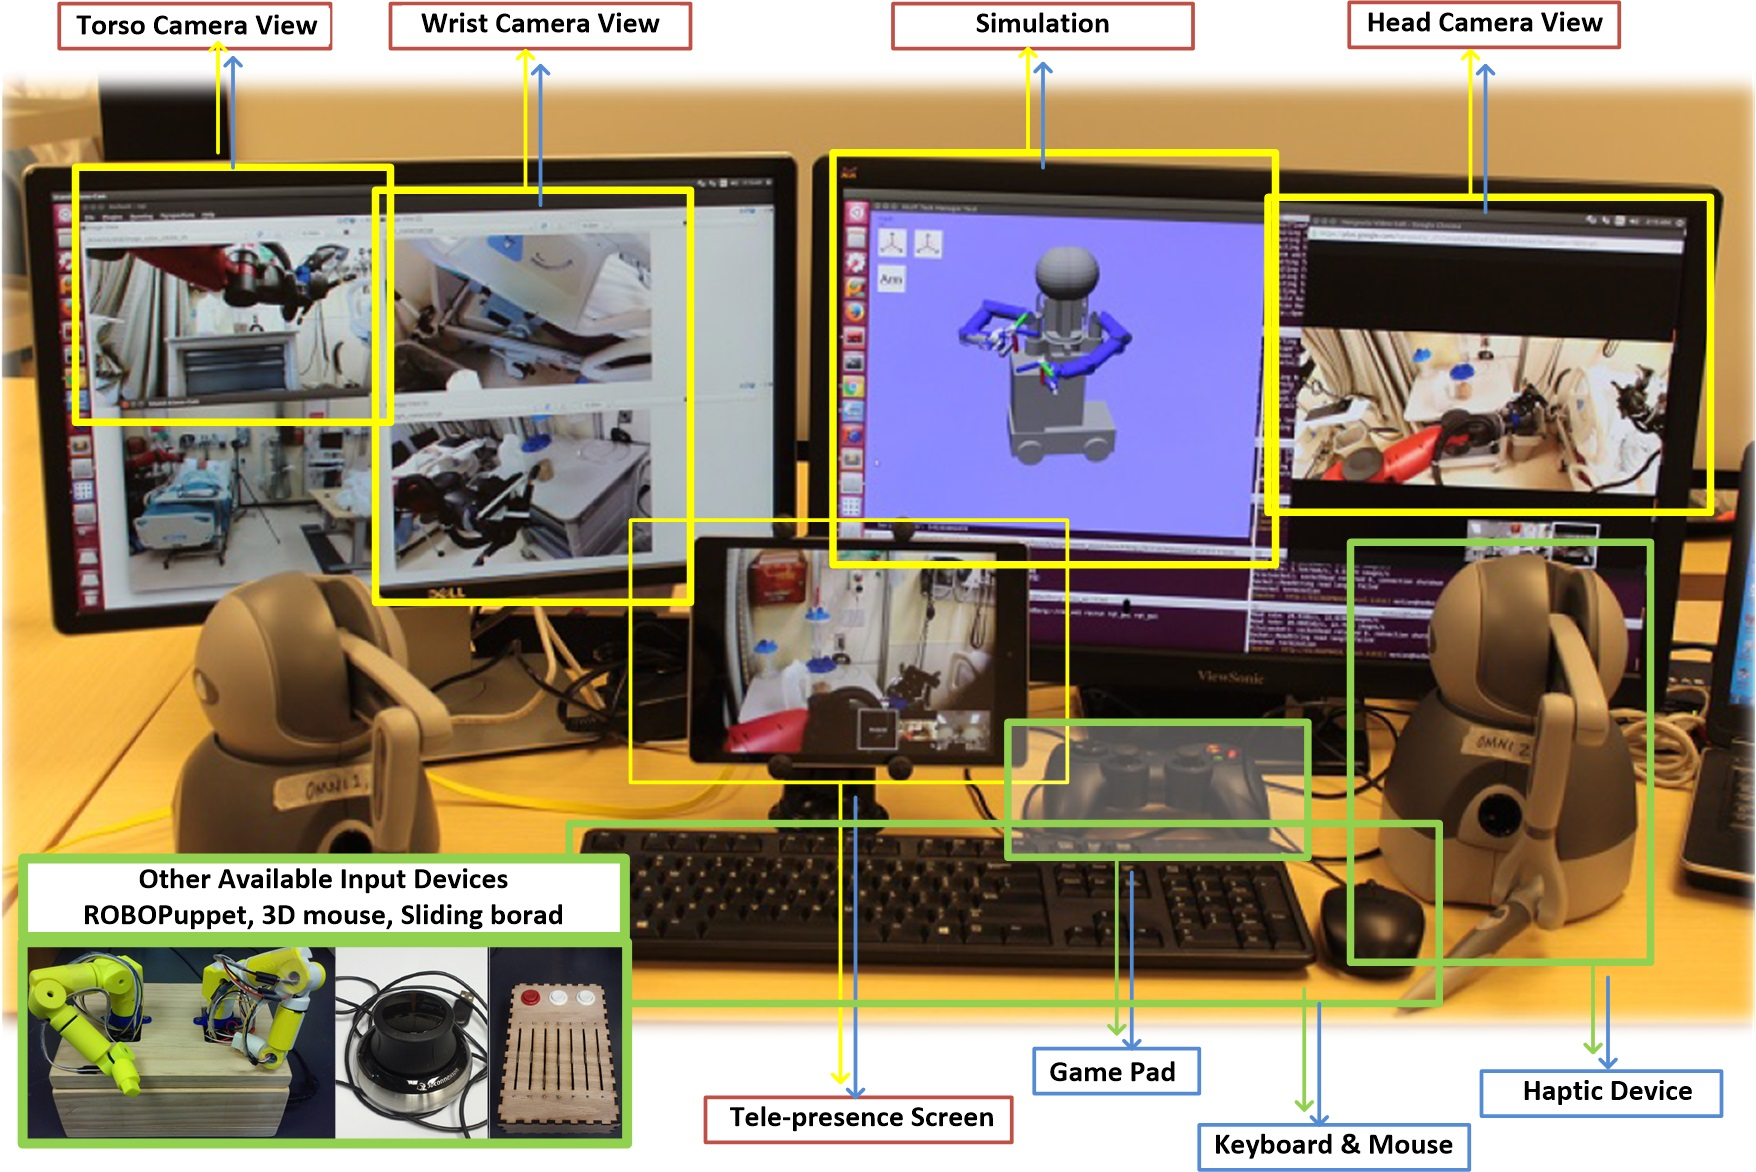
\includegraphics[width=0.48\linewidth]{fig//TRINA_Console_Notes}
}
    \caption{(Left) The Tele-robotic Intelligent Nursing Assistant (TRINA) system and (Right) its operator console which can support various modalities for direction teleoperation and shared-autonomous control.}
    \label{fig:Trina_facility}
\vspace{2ex}
\end{figure}

PI Li has a fully integrated Tele-robotic Intelligent Nursing Assistant (TRINA) system (see~\fig{fig:Trina_facility}). A Da Vinci surgical robot console is also available as an additional robot teaching interface. PIs Li and Fu share a Vicon motion capture system, with 10 Vicon Vero 2.2 cameras. PI Ziebart has a Rethink Robotics Baxter platform, Microsoft Kinect 3D cameras and an HTC Vive virtual reality system.

%-------------------------------------------------------------------------
\section{Computing Resources}\label{sec:Computers}
%-------------------------------------------------------------------------

\paragraph*{Computers} Li and Fu's lab has two desktop and one laptop computers dedicated for students work on this project. PI Ziebart has one workstation equipped with graphical processor units for running real-time robotics experiments, multiple servers for off-line machine learning tasks, and laptops for research assistant usage. In addition, WPI provides extensive computational resources including high speed networking, data hosting and storage and high-performance computing. Multiple platforms are available for unit testing software under different operating systems and hardware configurations. These shared computing resources can support intensive computing tasks as well as securely host data and project code. 

\paragraph*{Computer Software} 
Software for mechanical design and manufacturing, circuit board modeling and design, mathematical modeling, and software development are readily available. Workstations are available with all required programming, simulation, and modeling software and hardware. This resources can support robot platform maintenance, and develop robot accessories and experimental setups needed for system evaluation.  

%-------------------------------------------------------------------------
\section{Facility for user study and system evaluation}\label{sec:PracticePoint}
%-------------------------------------------------------------------------
The user study for system evaluation will be performed in the simulated patient room at the WPI PracticePoint. PracticePoint is a membership-based R\&D and commercialization alliance that seeks to improve healthcare technologies and develop new medical cyber-physical systems. PracticePoint will provide an agile and scalable, collaborative research facility empowering public and private universities, research institutions, industry and innovators to incorporate cyber-physical systems into medical devices and equipment that will improve performance, security, accuracy, timeliness, costs and outcomes in human healthcare. PracticePoint will foster professional collaborations among its members and partner institutions through four state-of-the-art test beds, secured project pods, collaboration suites and shared tool bays.

At the facility, members will have access to point-of-practice environments including: medical imaging coupled with a hybrid operating room suite (including an MRI scanner), a controlled care environment (reconfigurable as ICU, exam room, and recovery room), rehabilitative care suites (including motion capture and rehab equipment), and a residential setting (highly instrumented mock home environment). These point of practice care suites will be integrated with advanced manufacturing and testing equipment. It has advanced manufacturing (including CNC machining, 3D printing, laser cutting), electronics assembly and test equipment, and build areas. It will also comprise office spaces for faculty and graduate students, individual research group lab spaces, and reconfigurable “lab pods” that can be assigned to collaborating organizations or used on a short-term per-project basis. 



\pagebreak
\setcounter{page}{1}
\bibliographystyle{IEEEtran}
\bibliography{./ref,./jieref}

\end{document}
